\documentclass[10pt]{article}
\usepackage[a4paper, tmargin=0.75in, lmargin=0.80in, rmargin=0.80in, bmargin=1in]{geometry}
\usepackage{hyperref}
%\usepackage{multicol}
\hypersetup{
    colorlinks=true,
    linkcolor=black,
    filecolor=magenta,      
    urlcolor=blue,
    citecolor=black,
}
%\usepackage[numbers,sort&compress]{natbib} % for a numerical citation list
\usepackage{natbib} % to cite references by surname and year
\usepackage{graphicx}
\usepackage{subfigure}
\usepackage{amsmath}
\usepackage{lipsum}
\usepackage{url}
\usepackage{soul}
\usepackage[UTF8]{ctex}            %中文宏包
\usepackage{color, xcolor}         %字体颜色包
\usepackage[normalem]{ulem}        %支持删除线
\usepackage[dvipsnames]{xcolor}    %支持68种未预定义的颜色
\usepackage{float}                 %这三个包用于插入图片(后两个实现多张图片的并排插入)
\usepackage{enumerate}             %用于enumerate 列表中的自定义的标号
\usepackage[inline]{enumitem}      %内联列表,使列表嵌入文字中
\usepackage{tasks}                 %
\usepackage{amssymb}              %用于制考试选择题那样的水平列表
\usepackage{tabularx}
\usepackage{booktabs}
\usepackage{multirow}
\usepackage{algorithm}
\usepackage{algpseudocode}
\usepackage{hyperref}
\usepackage{caption, subcaption}
\graphicspath{{../figure/}}
\pagestyle{plain}


%%%%%%%%%%%%%%%%%%%%%%%%%%%%%%%%%%%%%%%%%%%%%%%%%%
%%%%%%%%%%%%%%%%%%%%%%%%%%%%%%%%%%%%%%%%%%%%%%%%%%
%%%%%%%%%%%%%%%%%%%%%%%%%%%%%%%%%%%%%%%%%%%%%%%%%%
%%%%%%%%%%%%%%%%%%%%%%%%%%%%%%%%%%%%%%%%%%%%%%%%%%
% ENTER SOME IMPORTANT INFORMATION
%%%%%%%%%%%%%%%%%%%%%%%%%%%%%%%%%%%%%%%%%%%%%%%%%%
%%%%%%%%%%%%%%%%%%%%%%%%%%%%%%%%%%%%%%%%%%%%%%%%%%
%%%%%%%%%%%%%%%%%%%%%%%%%%%%%%%%%%%%%%%%%%%%%%%%%%
%%%%%%%%%%%%%%%%%%%%%%%%%%%%%%%%%%%%%%%%%%%%%%%%%%
\newcommand{\studentname}{余俊洁}
\newcommand{\studentnumber}{523030910244}
\newcommand{\projecttitle}{机器学习大作业}
%%%%%%%%%%%%%%%%%%%%%%%%%%%%%%%%%%%%%%%%%%%%%%%%%%
%%%%%%%%%%%%%%%%%%%%%%%%%%%%%%%%%%%%%%%%%%%%%%%%%%
%%%%%%%%%%%%%%%%%%%%%%%%%%%%%%%%%%%%%%%%%%%%%%%%%%
%%%%%%%%%%%%%%%%%%%%%%%%%%%%%%%%%%%%%%%%%%%%%%%%%%
%%%%%%%%%%%%%%%%%%%%%%%%%%%%%%%%%%%%%%%%%%%%%%%%%%
%%%%%%%%%%%%%%%%%%%%%%%%%%%%%%%%%%%%%%%%%%%%%%%%%%

\begin{document}

\begin{center}
{\Huge{机器学习大作业报告}} \\
\vspace{2mm}
{\Large{SJTU}}
\end{center}

\vspace{5mm}
\hrule
\vspace{1mm}
\hrule

\vspace{3mm}
\begin{tabular}{ll} 
Name:           	        & {\studentname}   \\ 
Student Number: 	        & {\studentnumber} \\ 
Research Project Title: 	& {\projecttitle}  \\  
\end{tabular}

\vspace{3mm}
\hrule
\vspace{1mm}
\hrule

\tableofcontents
\newpage

\section{大作业概论}
本次机器学习大作业针对 2015-2019 年旅客出行数据,完成了对于停留天数(回归任务)和旅游目的(分类任务)两项预测任务。  
首先我对5年的原始数据进行了合并,清洗与归一化处理等工作;随后,我使用特征学习技术,分别对数据进行了针对回归任务的主成分分析(PCA)降维,和针对分类任务的线性判别分析(LDA)降维。  
在时间序列背景下,按照要求,使用 sklearn.model\_selection.TimeSeriesSplit(n\_splits = 5)对时间序列数据进行多折划分进行模型评估与网格化超参数搜索。  
其中,我使用的回归模型包括普通线性模型、L1(Lasso)、L2(Ridge)、随机森林和SVR;分类模型包括 KNN、Logistic回归、LDA、贝叶斯、SVM和随机森林。  
最后,对比分析了在不同的数据处理方式下,不同模型在多维指标上的表现,并讨论特征学习与正则化对模型稳定性的影响。
%-------------------------------------------------
\section{数据与任务描述}
\subsection{数据来源与字段简介}
数据包含 2015–2019 年共 (72370, 382) 组数据(将所有数据集合并之后的.shape)。主要特征组如下:
\begin{itemize}
  \item \textbf{类别变量}:包括游客的国籍、性别、旅行类型、最满意/最向往的地点、满意度水平等核心属性
  \item \textbf{数值变量}:包括游客的年龄、消费情况、旅游频次及多个旅游项目的满意度打分等
  \item \textbf{二值变量}:涉及游客在旅途中涉及的住宿、交通、活动、目的地、旅游动机及景点访问等行为特征
\end{itemize}

\subsection{预测任务}
\begin{description}
  \item[任务 1:] 回归 —— 预测连续型目标变量:旅客停留天数 (\emph{Number of nights in CITY})
  \item[任务 2:] 分类 —— 预测类别型目标变量:旅客旅游目的 (\emph{Purpose of visit to CITY})
\end{description}

%-------------------------------------------------
\section{数据预处理}
\begin{enumerate}
  \item \textbf{加载并合并数据: } 将2015年到2019年的所有数据合并并对其按照 `Survey date' 顺序排序。
  \item \textbf{定义特征类型: }分析数据,将数据分为类别变量,数值变量,二值变量三类。
  \item \textbf{缺失值处理:} 连续变量采用平均值填补,类别变量和二值变量采用众数填补。
  \item \textbf{类别编码:} One‑Hot(保留稀疏性)。
  \item \textbf{训练数据构建: }  构建用于回归和分类任务的训练数据,根据目标变量是否缺失来筛选样本,并构建特征 (X) 和目标变量 (y)。
  \item \textbf{标准化:} 对特征数据进行 Z-score 标准化,以提高模型训练的效果和稳定性。
\end{enumerate}

%-------------------------------------------------
\section{特征学习}

降维或特征学习的目标是从原始特征 $\mathbf{X}_{\text{orig}}\in\mathbb{R}^{n\times p}$ 中提取更具代表性的信息,提升模型性能与泛化能力。在实验中,我采用了三种主流特征学习方法:PCA、LDA 以及基于统计评分的SelectKBest,分别用于回归和分类任务。

\subsection{PCA (回归任务)}

PCA 通过线性变换将高维特征空间投影到低维空间,并尽可能保留原始数据的方差信息:
\[
  \mathbf{Z}_{\text{PCA}} = \mathbf{X}_{\text{orig}}\mathbf{W}_{k}, \quad
  \mathbf{W}_{k} = \arg\max \limits_{\mathbf{W}^\top\mathbf{W}=I}\operatorname{Var}(\mathbf{X}\mathbf{W})
\]
对于回归任务的数据,我采用了PCA降维,在多次尝试之后,最终选定降维后的特征维度为20。

\subsection{LDA (分类任务)}

LDA 利用类别标签信息,在类别间最大化区分度的同时最小化类别内差异。目标函数如下:
\[
  \mathbf{W}_{\text{LDA}} = \arg\max \limits_{\mathbf{W}} \frac{\det\left(\mathbf{W}^\top S_B \mathbf{W}\right)}{\det\left(\mathbf{W}^\top S_W \mathbf{W}\right)}
\]
其中 $S_B$ 和 $S_W$ 分别为类间散度矩阵和类内散度矩阵。对于分类任务的数据,我采用了LDA降维,由于 LDA 输出维度上限为 类别数$-1$,本任务共有4类,因此输出维度为 $3$。

\subsection{SelectKBest(回归与分类任务)}

SelectKBest 是一种基于统计检验的特征选择方法,通过评分函数评估每个特征与目标变量的相关性,选择得分最高的前 $k$ 个特征。本文采用了两种评分函数:

\begin{itemize}
  \item 回归任务使用 \textbf{F-statistic}(\texttt{f\_regression}),评估每个特征与目标变量之间的线性相关性。
  \item 分类任务使用 \textbf{ANOVA F值}(\texttt{f\_classif}),评估每个特征对类别标签的区分能力。
\end{itemize}

为比较不同的k的选择下的效果,我在实验中设置了两个 $k$ 值:$k=10$ 与 $k=50$,并分别构建了回归和分类任务下的特征子集 $\mathbf{X}_{\text{KBest}}$。

\vspace{0.8cm}

\noindent \hl{注 }:

当我在用上述数据训练模型时发现,会有一些极端值影响模型的效果,因而我们需要对那些极端值进行筛选,我尝试过直接对原始数据集进行极端值过滤,但是原始数据拥有382个维度,筛选过程消耗了大量不必要的算力,更重要的是,很多数据可能因为一些在那些不那么重要的数据上的离群值而被排除,进而损失了大量的有效的数据。

因此,我考虑在我得到的SelectKBest的数据集上进行按Z-score的异常值清洗,这样能够更为精准地去除那些我们不需要的数据且复杂度更低。同时,在实验中发现,对于k=10或50,两者的效果接近,k=10略胜一筹且复杂度更低,故实验中选取的极端值清洗后的数据集是基于k=10的特征提取数据集的。

\section{实验数据集合集 }
经过数据预处理和特征学习过程,选取得到以下进行实验的数据集:

\begin{itemize}
  \item 回归任务:
    \begin{itemize}
      \item $\mathbf{X}^{\text{(reg-ini)}} \in \mathbb{R}^{n \times p}$,原始数据;
      \item $\mathbf{X}^{\text{(reg-sca)}} \in \mathbb{R}^{n \times p}$,标准化后的数据;
      \item $\mathbf{X}^{\text{(reg-pca)}} \in \mathbb{R}^{n \times 20}$,PCA后的数据(经过标准化);
      \item $\mathbf{X}^{\text{(reg-selected)}}_{10} \in \mathbb{R}^{n \times 10}$,10个主要特征提取后的数据;
      \item $\mathbf{X}^{\text{(reg-selected)}}_{50} \in \mathbb{R}^{n \times 50}$,50个主要特征提取后的数据;
      \item $\mathbf{X}^{\text{(reg-selected-cleaned)}}_{10} \in \mathbb{R}^{n' \times 10}$,Z-score清洗后的10特征提取数据。
    \end{itemize}
  
  \item 分类任务:
    \begin{itemize}
      \item $\mathbf{X}^{\text{(cls-ini)}} \in \mathbb{R}^{m \times p}$,原始数据;
      \item $\mathbf{X}^{\text{(cls-sca)}} \in \mathbb{R}^{m \times p}$,标准化后的数据;
      \item $\mathbf{X}^{\text{(cls-lda)}} \in \mathbb{R}^{m \times 3}$,LDA后的数据(经过标准化);
      \item $\mathbf{X}^{\text{(cls-selected)}}_{10} \in \mathbb{R}^{m \times 10}$,10个主要特征提取后的数据;
      \item $\mathbf{X}^{\text{(cls-selected)}}_{50} \in \mathbb{R}^{m \times 50}$,50个主要特征提取后的数据;
      \item $\mathbf{X}^{\text{(cls-selected-cleaned)}}_{10} \in \mathbb{R}^{m' \times 10}$,Z-score清洗后的10特征提取数据。
    \end{itemize}
\end{itemize}

其中 $n,m$ 为原始样本数,$n',m'$ 为极端值清洗后样本数。
%-------------------------------------------------
\section{实验设计}
\subsection{滚动预测策略}
滚动预测策略的目的是将数据划分为多个训练集和测试集,其中每次的训练集包含了当前时间点之前的数据,而测试集则包含了之后的数据,这样能够有效模拟实际的预测场景,即利用过去的数据预测未来的趋势。

在实验中,按照要求,我使用$sklearn.model\_selection.TimeSeriesSplit(n\_splits = 5)$来进行时间序列的交叉验证,根据第一列数据变量Survey date对数据进行切片。
\begin{algorithm}[H]
  \caption{五折滚动预测}
  \begin{algorithmic}[1]
    \State 设时间序列样本按日期升序排列
    \For{$i = 1$ \textbf{to} $5$}
      \State 使用前 $i$ 个时间窗口作为训练集,下一窗口作为验证集
      \State 进行网格搜索 \& 模型训练
      \State 记录折内最佳模型及性能
    \EndFor
    \State 计算网格索搜得到的最佳参数对应模型所有折指标的平均值
  \end{algorithmic}
\end{algorithm}

\subsection{超参数网格}
\subsubsection{回归模型}
\begin{table}[H]\centering
  \caption{回归模型与超参数网格}
  \begin{tabular}{ll}
    \toprule
    模型 & 网格超参数 \\ \midrule
    线性模型 & — \\
    Lasso(L1正则) & $\alpha \in \{10^{-2},10^{-1},10^{0},10^{1}\}$ \\
    Ridge(L2正则) & $\alpha \in \{10^{-2},10^{-1},10^{0},10^{1}\}$ \\
    SVR & $C\in\{0.1,1,10\}$,\  $\epsilon\in\{10^{-2},10^{-1}\}$,\ $\text{kernel}\in\{`linear',`rbf'\}$ \\
    RandomForest & $\text{n\_estimators}\in\{100,200\}$,\  $\text{max\_depth}\in\{5,10,None\}$,\  $\text{min\_samples\_split}\in\{2,5\}$ \\
    \bottomrule
  \end{tabular}
\end{table}

\subsubsection{分类模型}
\begin{table}[H]\centering
  \caption{分类模型与超参数网格}
  \begin{tabular}{ll}
    \toprule
    模型 & 网格超参数 \\ \midrule
    KNN & $k\in\{3,5,7,9\}$,\ $\text{weights}\in \{`uniform',`distance'\}$,\ $p\in\{1,2\}$ \\
    Logistic & $C\in\{0.01,0.1,1,10\}$,\  $\text{penalty} = \{l1,l2\}$ \\
    LDA (Classifier) & $\text{solver}\in\{`svd',`lsqr',`eigen'\}$,\ $\text{shrinkage}\in\{auto,0.1,0.2,0.3\}$ \\
    GaussianNB(贝叶斯) & var\_smoothing $\in[10^{-9},10^{-8},10^{-7}]$ \\
    SVM & $C\in\{0.1,1,10\}$,\ $\text{kernel}\in\{`linear',`rbf'\}$,\ $\gamma \in \{`scale',`auto'\}$ \\
    RandomForest & $\text{n\_estimators}\in\{100,200\}$,\  $\text{max\_depth}\in\{5,10,None\}$,\  $\text{min\_samples\_split}\in\{2,5\}$ \\
    \bottomrule
  \end{tabular}
\end{table}

\subsection{评估指标}
\subsubsection*{回归}
\begin{equation}
  \text{MSE} = \frac{1}{n}\sum_{i=1}^{n}(y_i - \hat{y}_i)^2,\quad
  \text{MAE} = \frac{1}{n}\sum_{i=1}^{n}|y_i - \hat{y}_i|, \quad
  R^2 = 1-\frac{\sum_{i}(y_i-\hat{y}_i)^2}{\sum_{i}(y_i-\bar{y})^2}
\end{equation}
选择这些指标,能较好地反映模型对于大误差的敏感性(MSE)、整体稳健性(MAE)和拟合能力(R2)。
\subsubsection*{分类}
分别采用宏平均与加权平均的 Accuracy / Precision / Recall / F1,以及 \textsc{OvR} AUC,
以全面评估模型的整体表现与各类识别能力。

同时实验结果的详细信息中给出了macro和weighted两种取平均的方式,但在下一节的整体汇总中仅展示了weighted的结果,是因为按使用样本量加权的方式,能更真实地反映总体性能,避免被少数类扭曲,也更符合实际的要求。
\subsection{可视化}
\subsubsection*{回归}
\begin{itemize}
  \item 数据实际值与预测值对比图
  \item 不同模型在不同的数据集下的评价指标条形图
  \item 不同模型在不同数据集下得到的不同评估指标的热力图
  \item R2雷达图
  \item MSE,MAE,R2气泡图
  \item MSE,MAE,R2平行坐标图
\end{itemize}

\subsubsection*{分类}
\begin{itemize}
  \item 不同模型在不同的数据集下的各个评价指标条形图
  \item Accuracy雷达图
  \item 混淆矩阵(Confusion Matrix)
  \item 不同类别的ROC曲线
\end{itemize}
%-------------------------------------------------
\newpage
\section{实验结果与分析}
\subsection{回归任务结果与分析}
\paragraph{结果}
\noindent \hl{注 }:不同模型在不同数据集下的具体的数据请参考附录A.

将所有的实验数据进行归纳,得到以下三种评价指标的可视化呈现:
\begin{figure}[H]
  \centering
  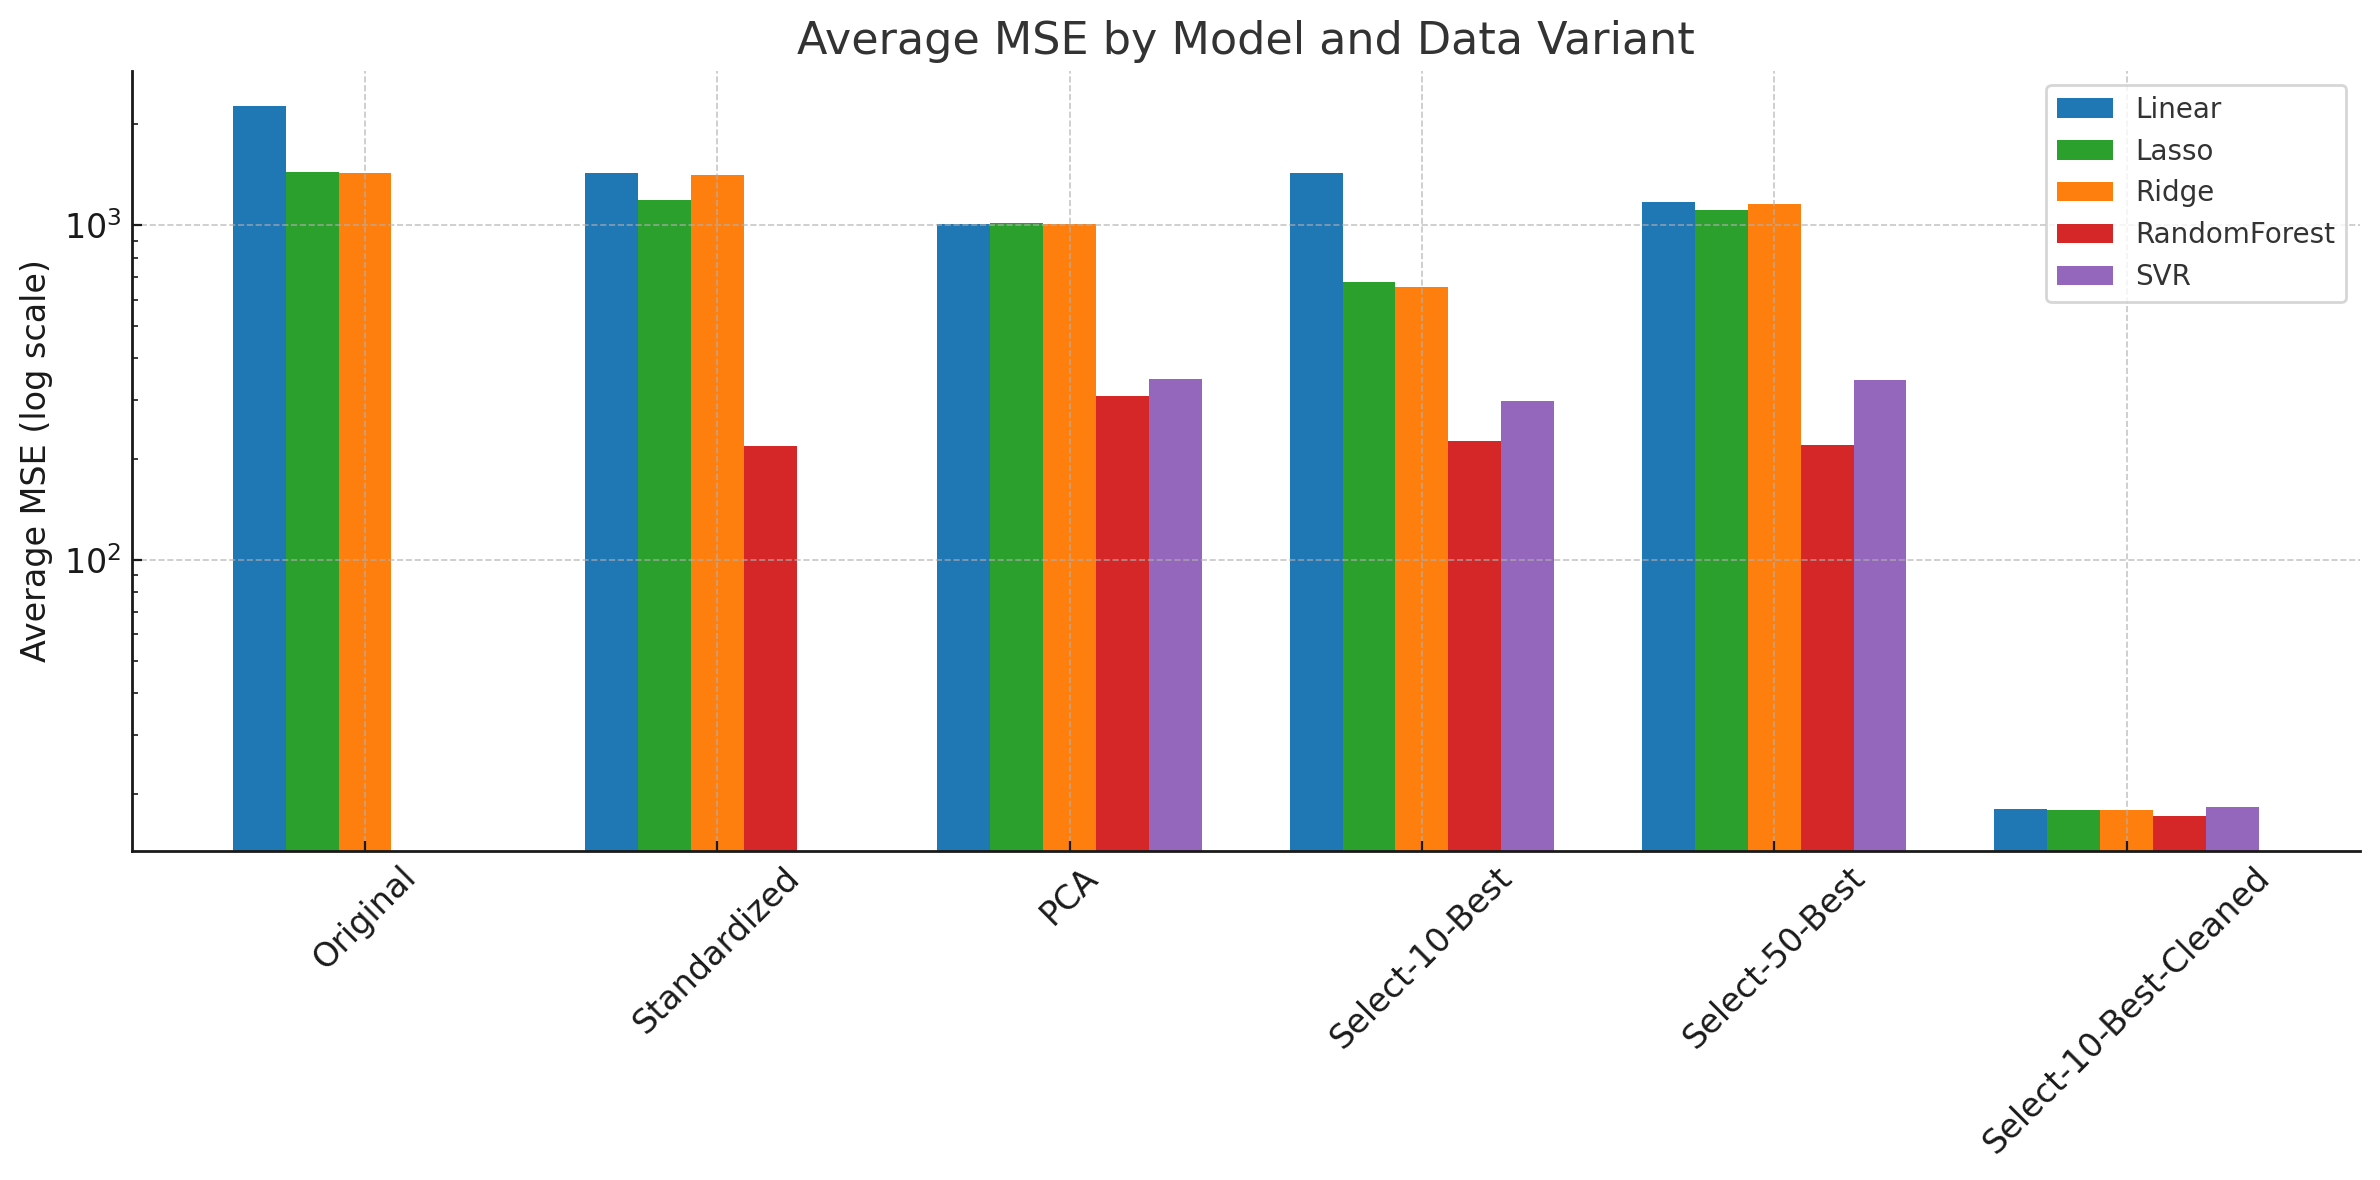
\includegraphics[width=0.8\linewidth]{average_mse.png}
  \label{fig:1}
\end{figure}
\begin{figure}[H]
  \centering
  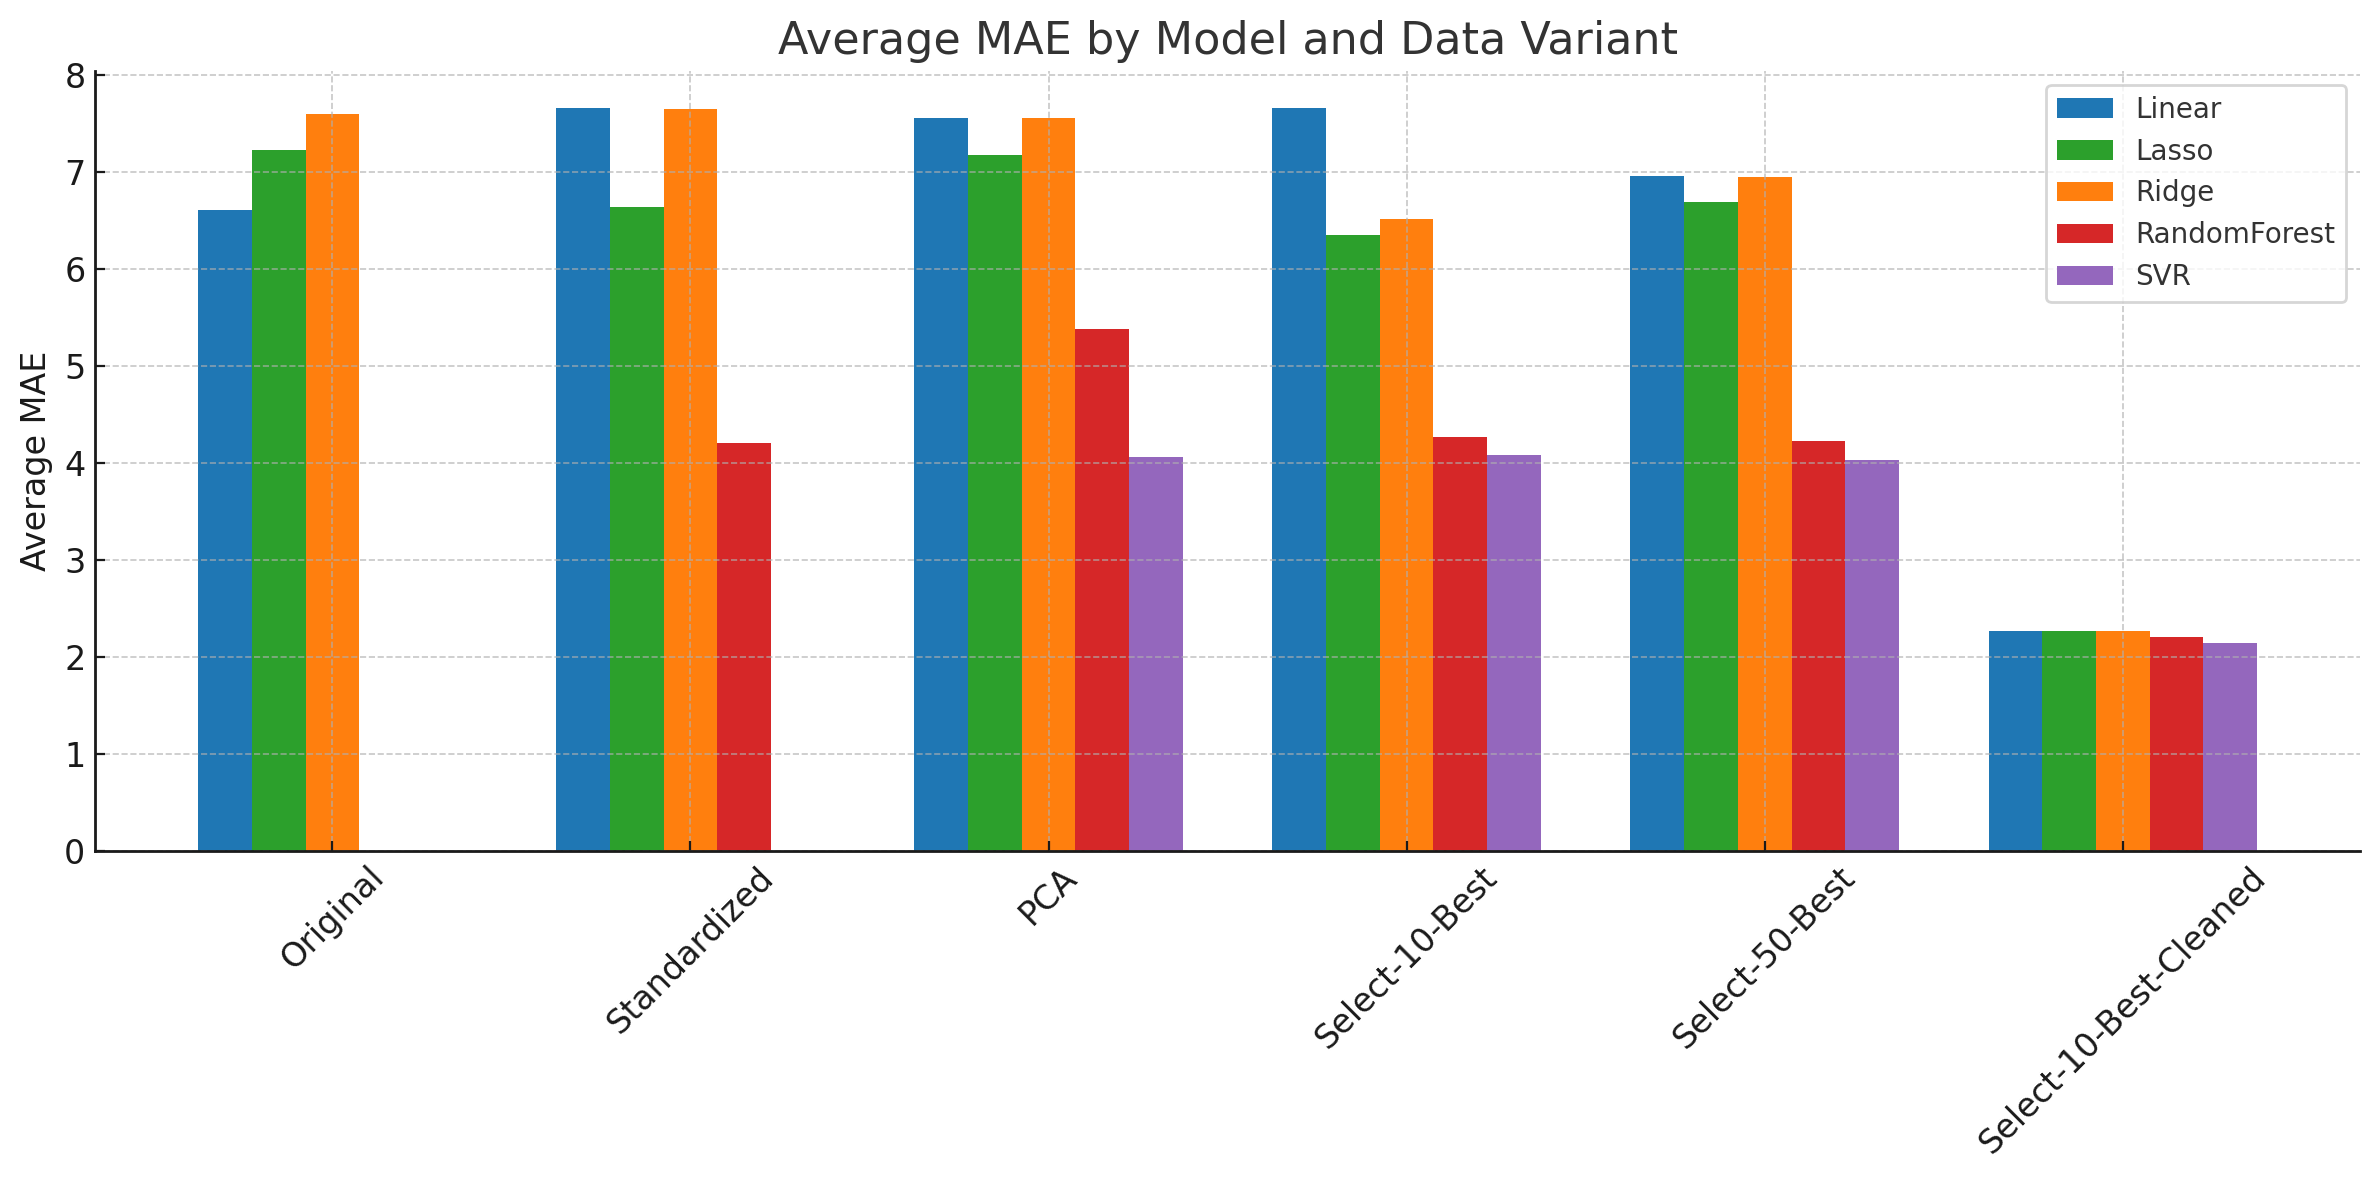
\includegraphics[width=0.8\linewidth]{average_mae.png}
  \label{fig:2}
\end{figure}
\begin{figure}[H]
  \centering
  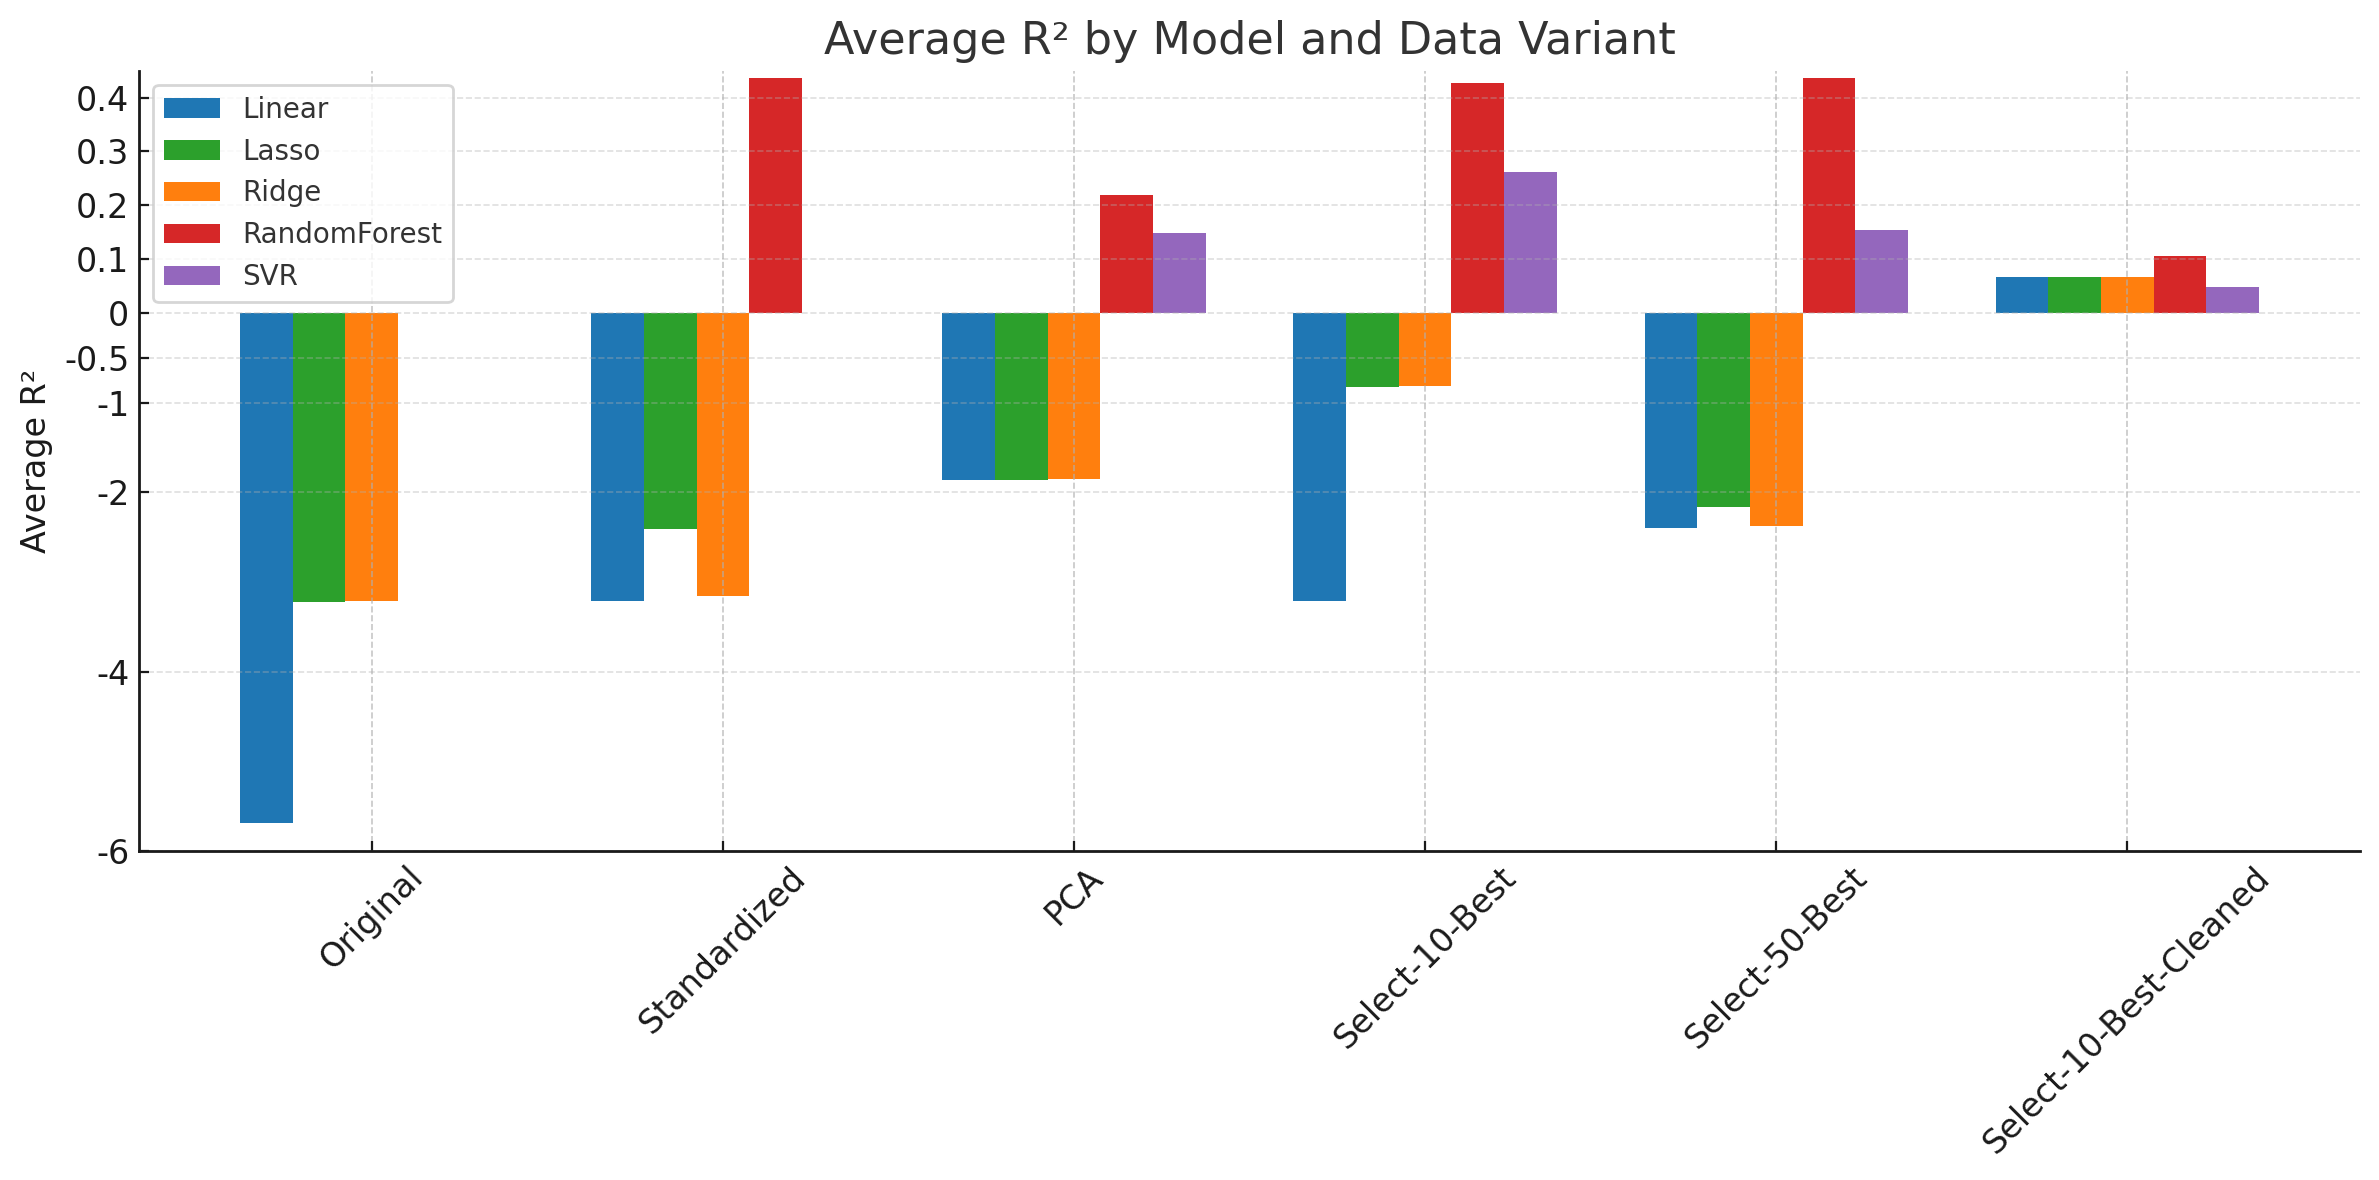
\includegraphics[width=0.8\linewidth]{average_R2.png}
  \label{fig:3}
\end{figure}

更为直观地,我绘制了不同模型在不同数据集下得到的不同评估指标的热力图:
\begin{figure}[H]
  \centering
  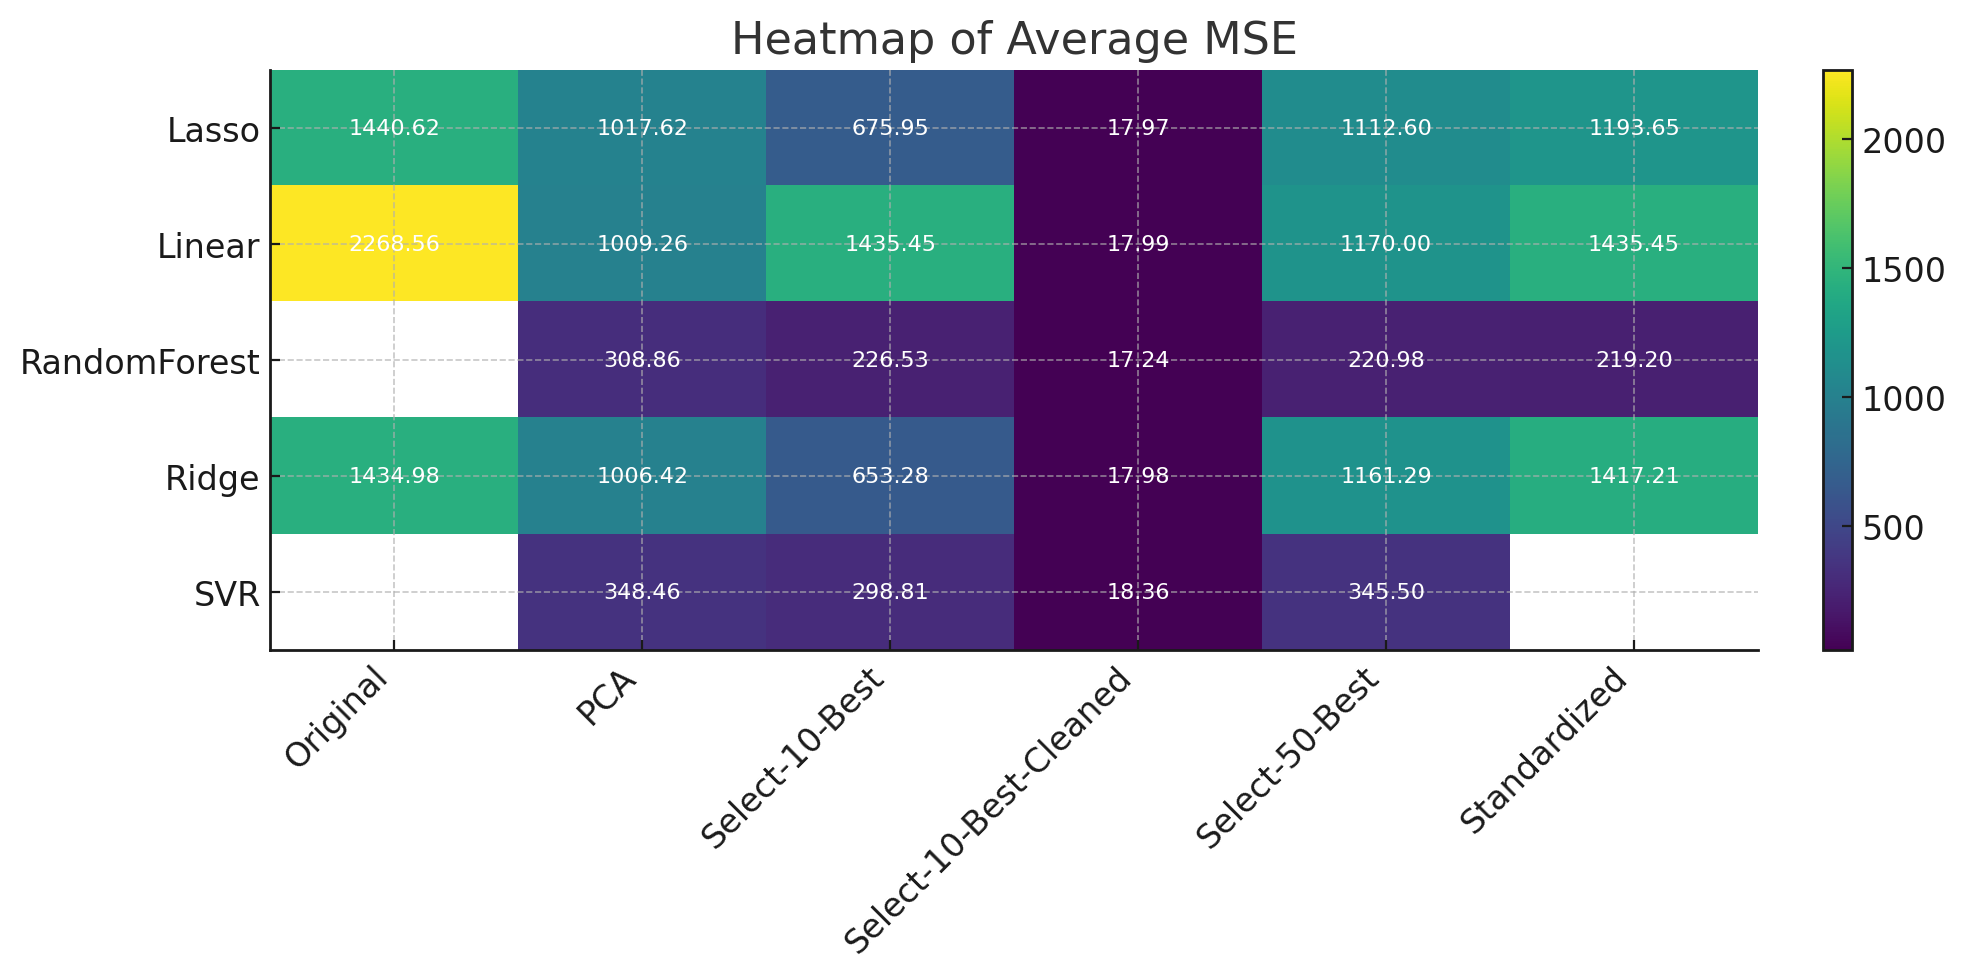
\includegraphics[width=0.8\linewidth]{heatmap_MSE.png}
  \label{fig:4}
\end{figure}
\begin{figure}[H]
  \centering
  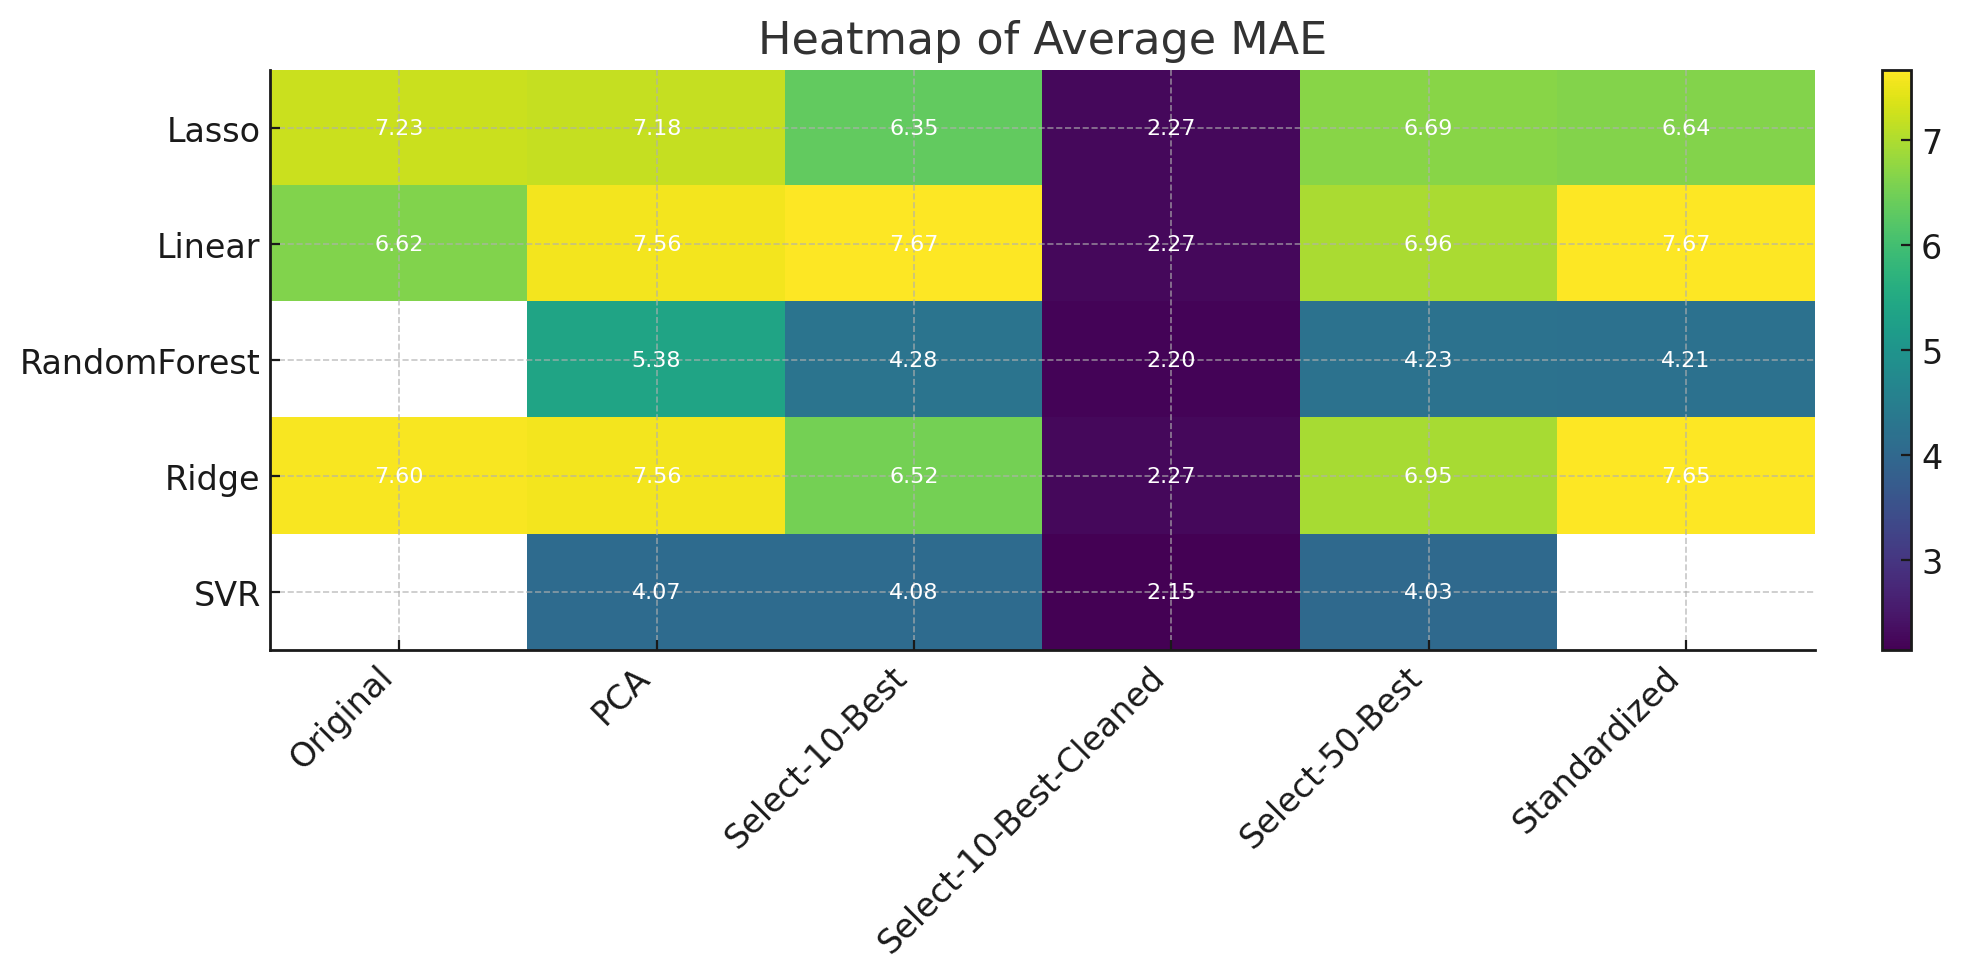
\includegraphics[width=0.8\linewidth]{heatmap_MAE.png}
  \label{fig:5}
\end{figure}
\begin{figure}[H]
  \centering
  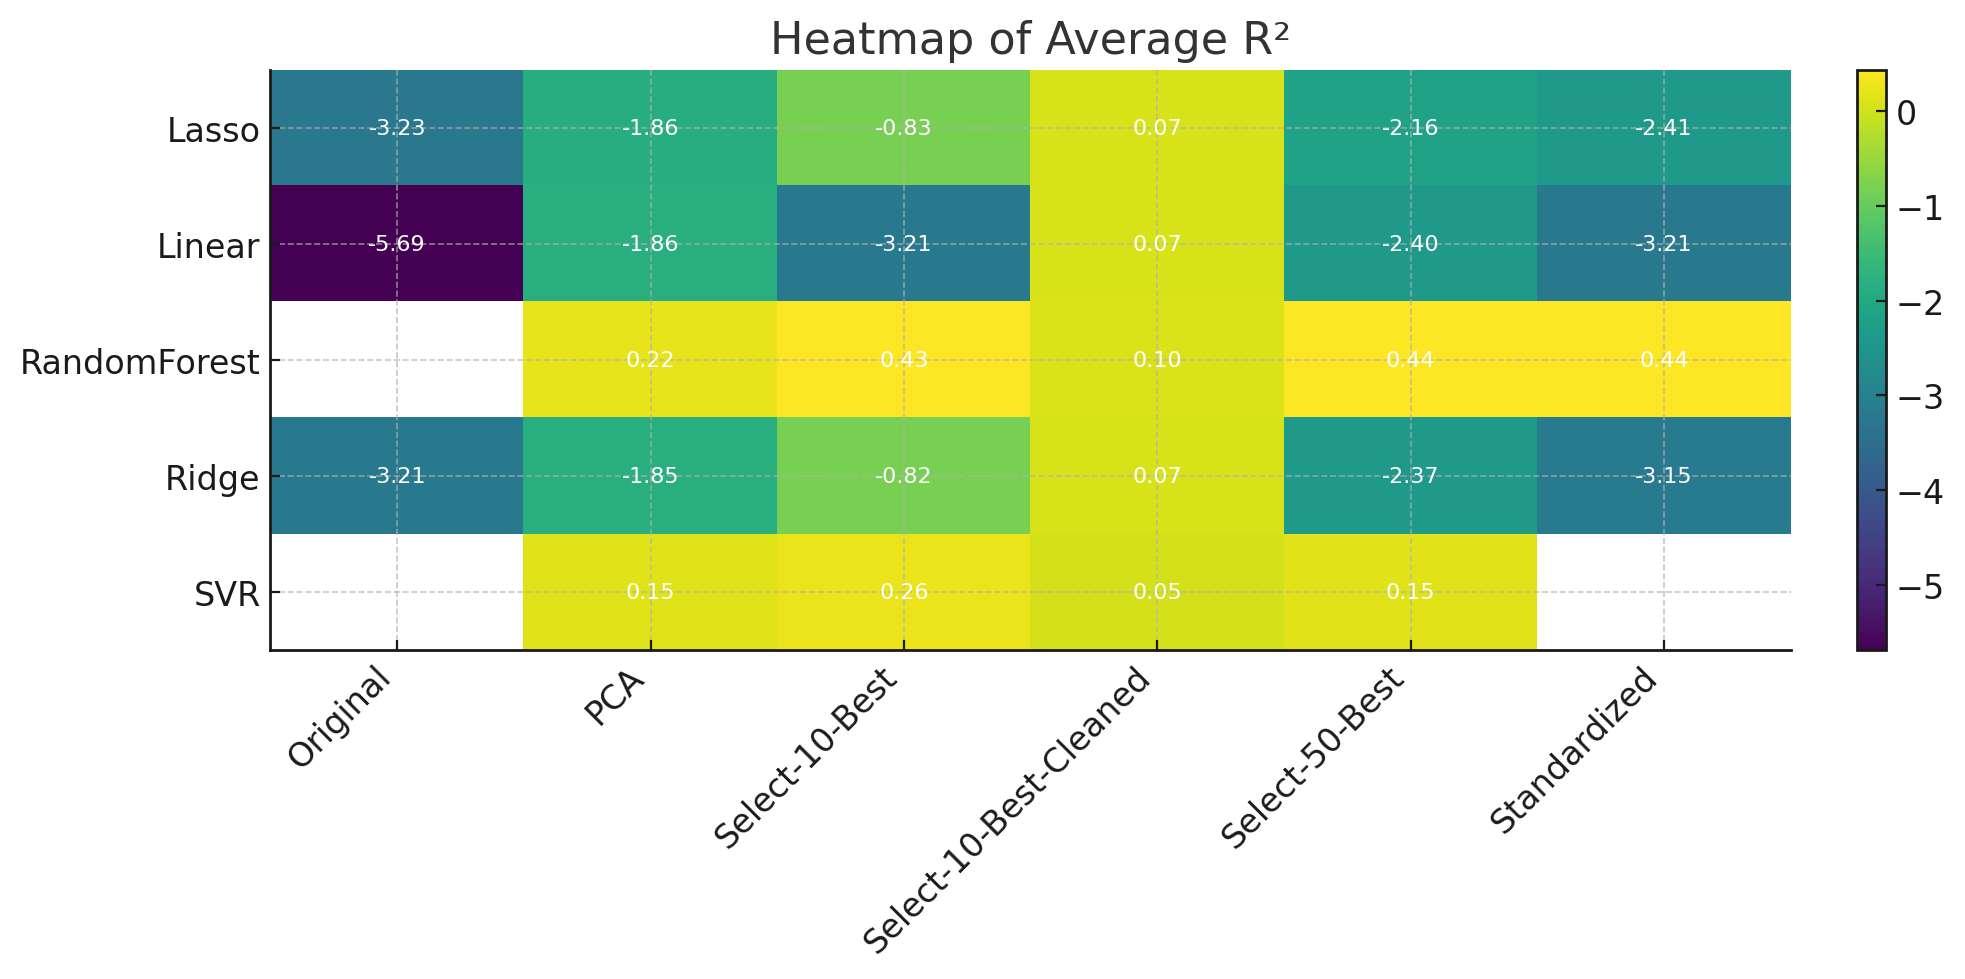
\includegraphics[width=0.8\linewidth]{heatmap_R2.png}
  \label{fig:6}
\end{figure}
同时,通过绘制R2的雷达图,我们也能更为清晰地比较各模型的性能:
\begin{figure}[H]
  \centering
  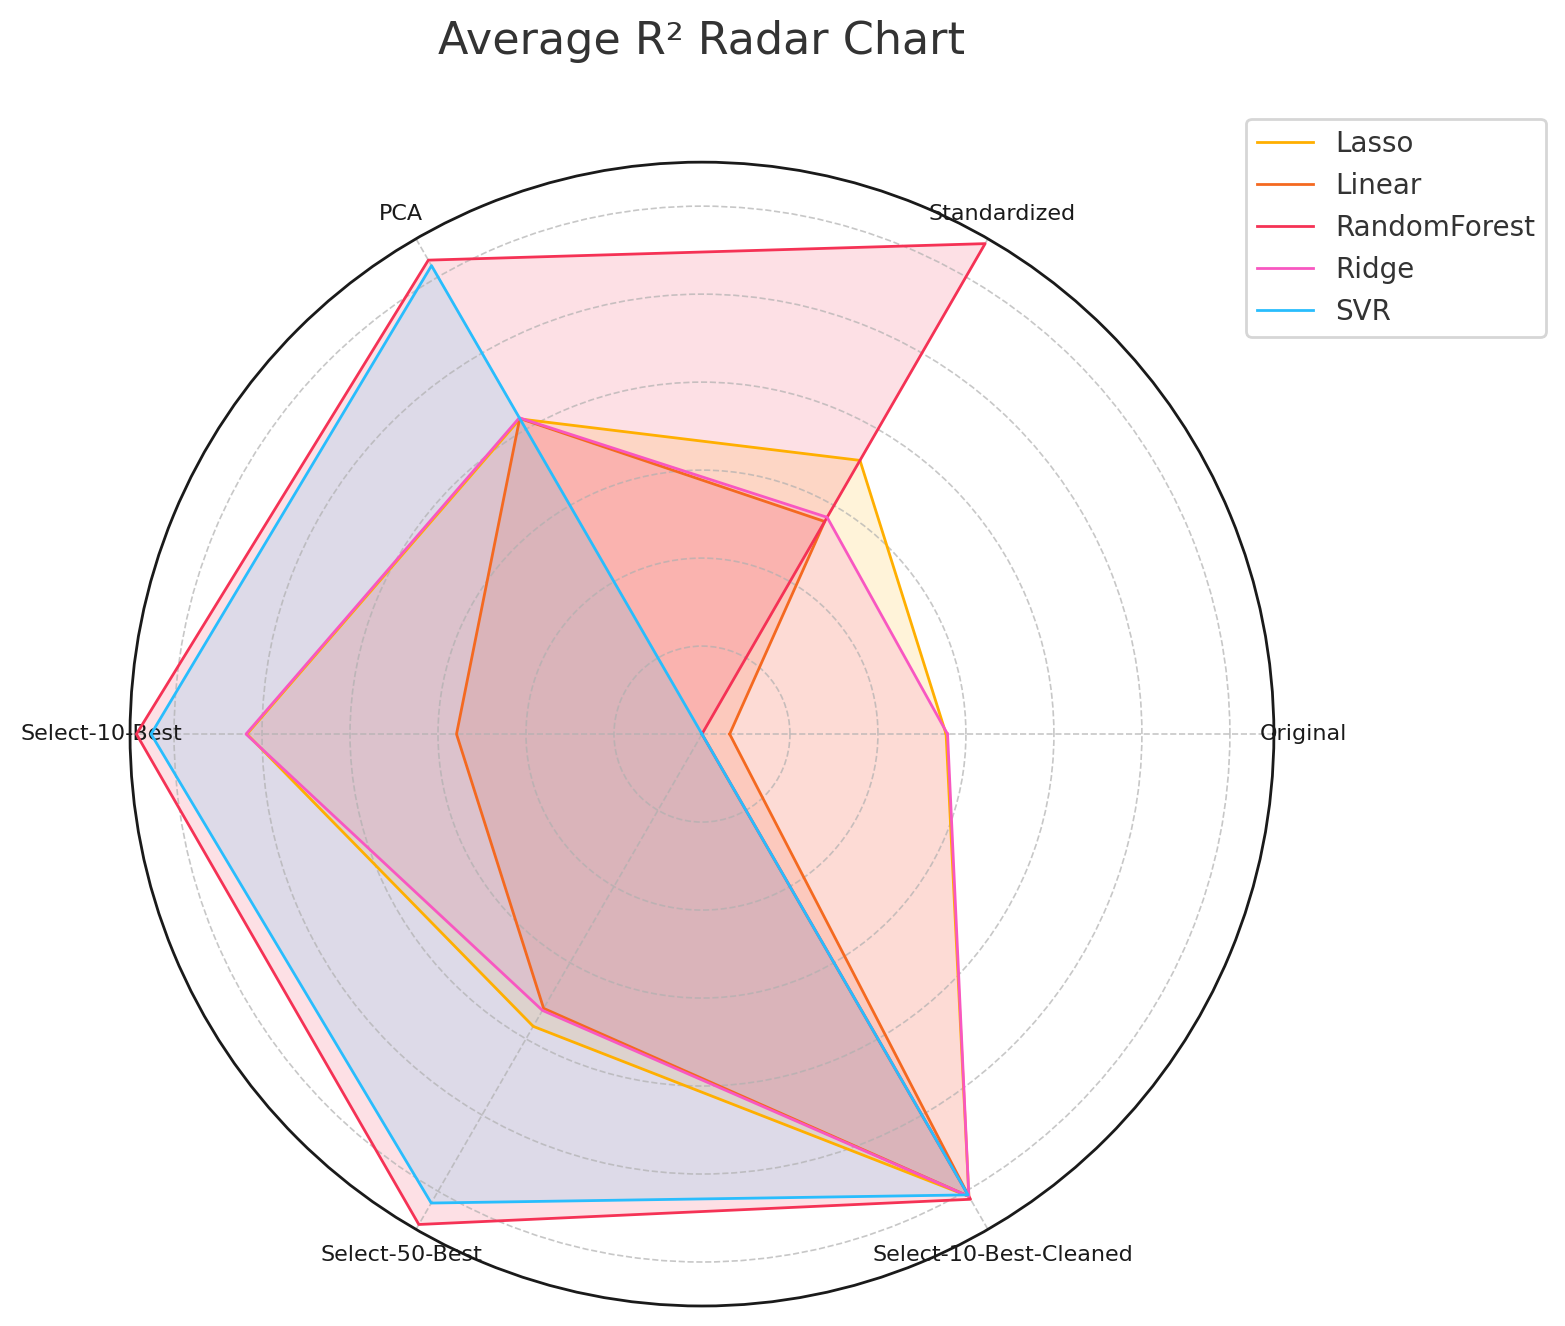
\includegraphics[width=0.7\linewidth]{radar_r2.png}
  \label{fig:7}
\end{figure}
同时把MSE,MAE和R²(气泡大小与颜色)映射到一张图上,得到三者的气泡图,更为便捷地观察模型‑数据组合误差大小、拟合好坏:
\begin{figure}[H]
  \centering
  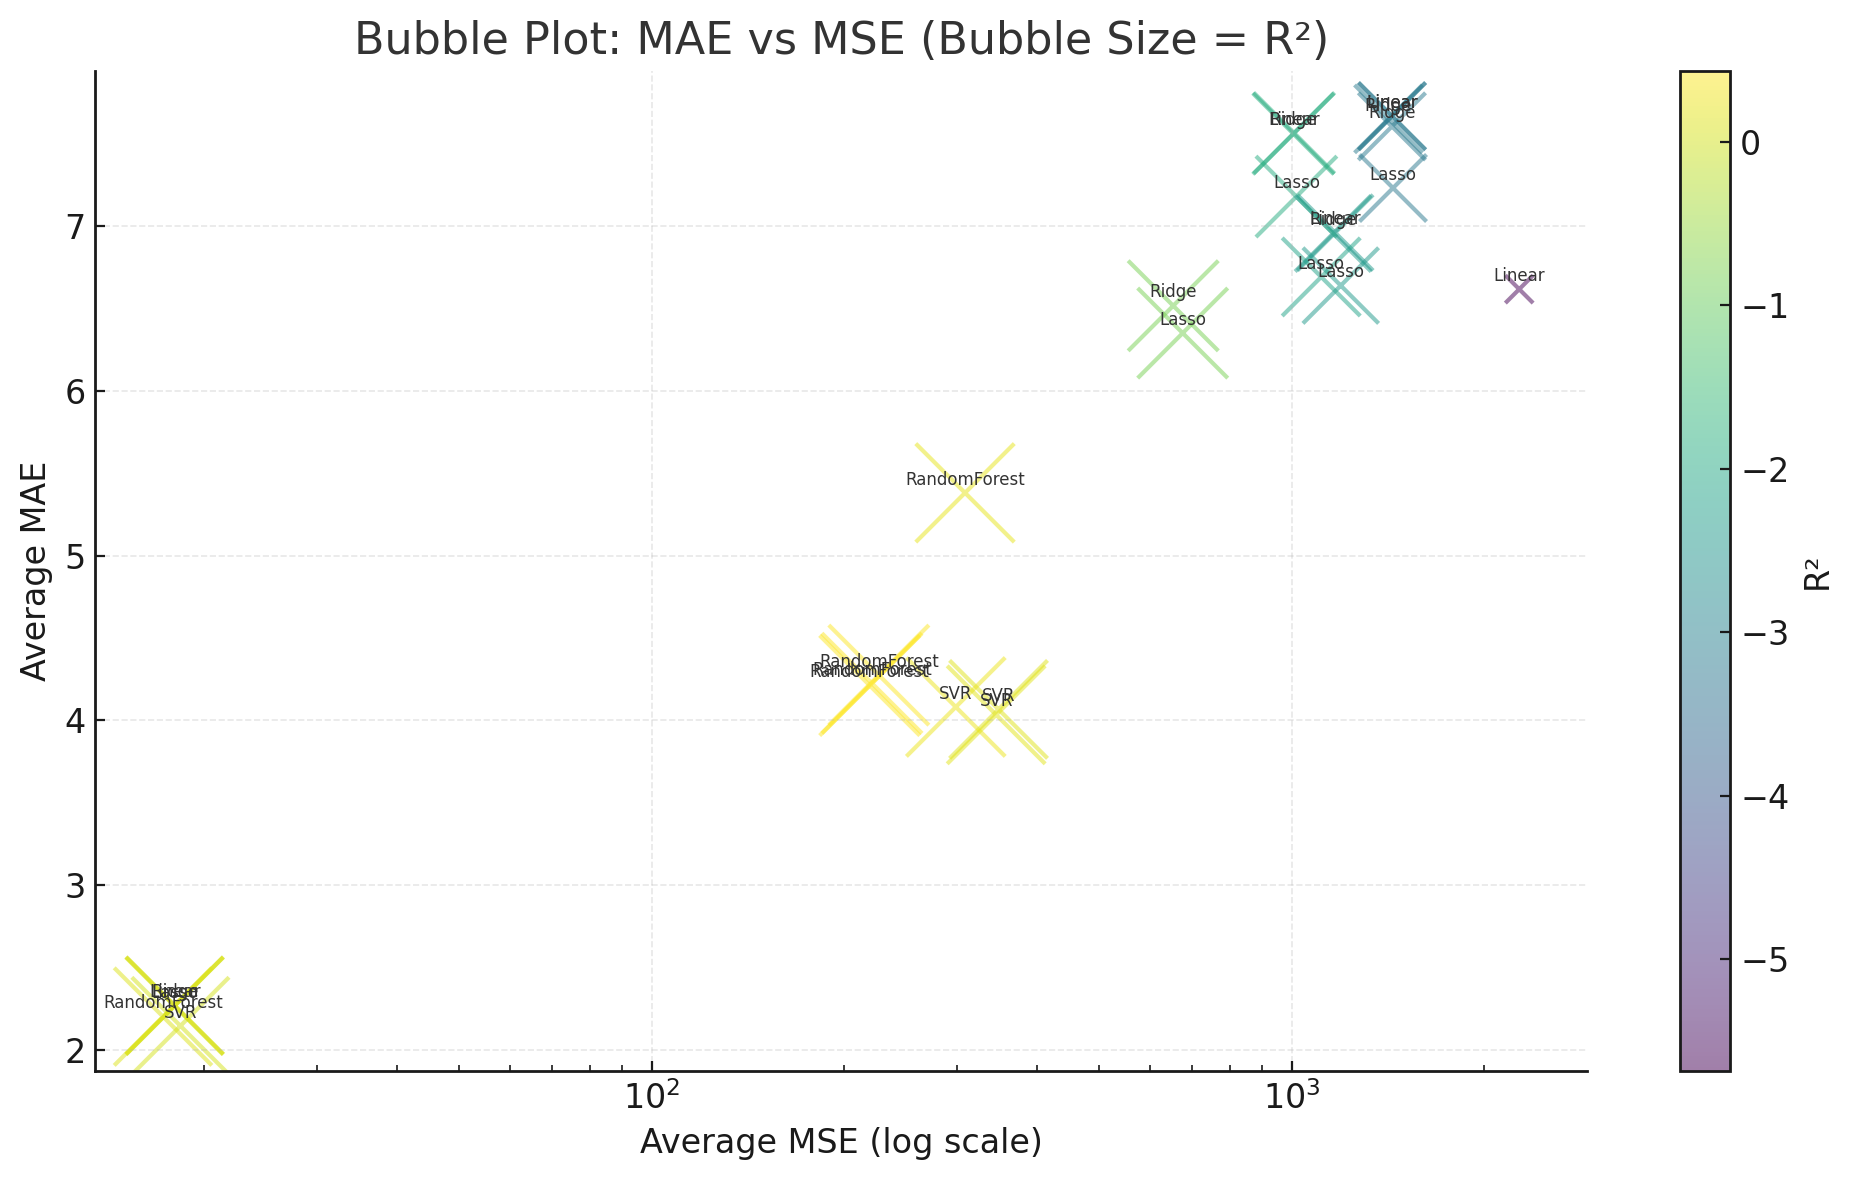
\includegraphics[width=0.8\linewidth]{bubble_plot.png}
  \label{fig:8}
\end{figure}
为了直观揭示多指标之间的权衡与优势走向,我把各组合在 MSE、MAE、R² 三条坐标轴上的归一化数值连成折线,绘制得到平行坐标图:
\begin{figure}[H]
  \centering
  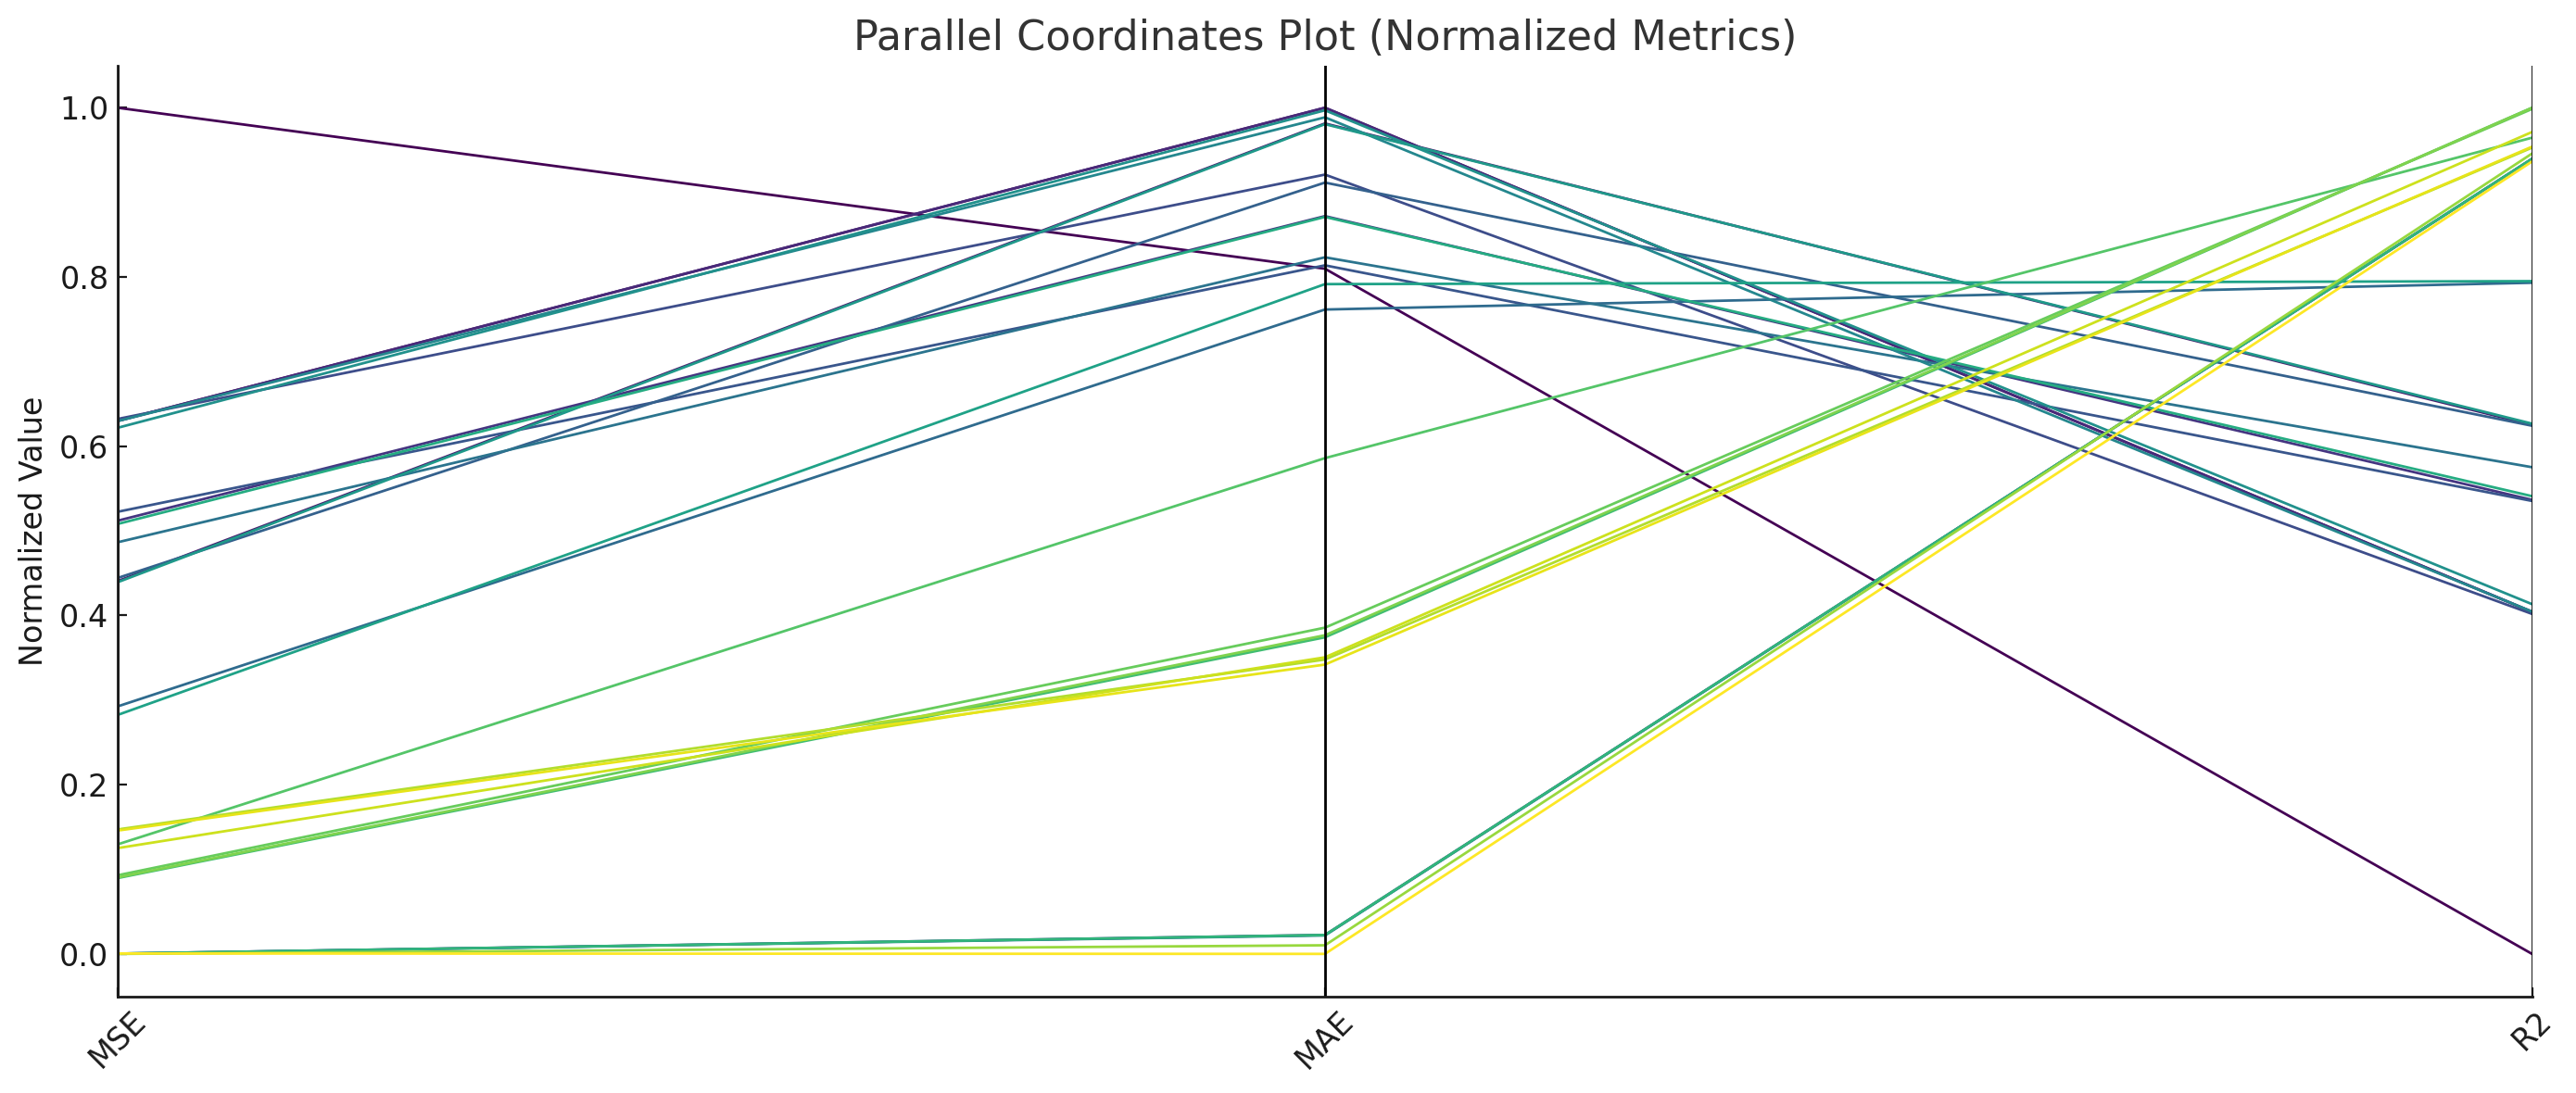
\includegraphics[width=0.8\linewidth]{parral.png}
  \label{fig:9}
\end{figure}
\paragraph{分析}  
\begin{itemize}
  \item 模型的适应性与复杂性
  \begin{itemize}
    \item 线性模型与正则化(Lasso、Ridge):虽然这些模型整体的效果很难比得上像随机森林一样的复杂模型,但其的复杂度较低。在数据特征较简单、线性相关性强的情况下表现尚可,然而,在面对高维复杂数据时(如实验中的未经过PCA或特征选择的数据集),这些模型的效果就不太令人满意了。特别是当我在进行Lasso的超参数调节时,$\alpha$值过小时,出现了过拟合现象。
    \item 随机森林回归模型:其优异表现的根本原因在于其对非线性关系和高维数据的处理能力。其通过多决策树的集成,有效减少了模型对噪声的敏感性。相比其他回归模型,其对特征选择后的数据表现更为稳定,具有较强的泛化能力。
  \end{itemize}
  \item 特征工程对回归性能的影响
  \begin{itemize}
    \item PCA的降维:PCA通过减少特征空间维度,有助于减轻计算负担,尤其是在处理高维数据时。然而,这种降维方法并没有在所有模型中带来提升,比如随机森林在PCA数据下训练的效果反而还不如直接在标准化后数据下训练的效果,可能在PCA的过程中丢失一些对回归任务至关重要的信息,而影响了模型的效果。
    \item 在进行极端异常值的清理之后,我发现,所有模型的R2均为正了,表明了对于极端离群值的去除能够显著地减少很多干扰,而使得模型的训练效果提升。
    \item 特征选择(SelectKBest):特征选择帮助剔除不重要的特征,从而降低了数据的噪声水平,提升了回归模型的效果,也很大程度地提高了模型的训练速度。
  \end{itemize}
  \item 超参数与正则化的敏感性
  \begin{itemize}
    \item 在实验的过程中,我发现SVR在不同的C和ϵ值设置下,表现波动较大,可见超参数调优的重要性。
  \end{itemize}
\end{itemize}

\subsection{分类任务结果与分析}
\paragraph{结果}
\noindent \hl{注 }:不同模型在不同数据集下的具体的数据与对应的混淆矩阵请参考附录A.

将所有的实验数据进行归纳,得到以下指标(Accuracy,Precision(weighted),Recall(weighted),F1-score(weighted),AUC)的可视化呈现:
\begin{figure}[H]
  \centering
  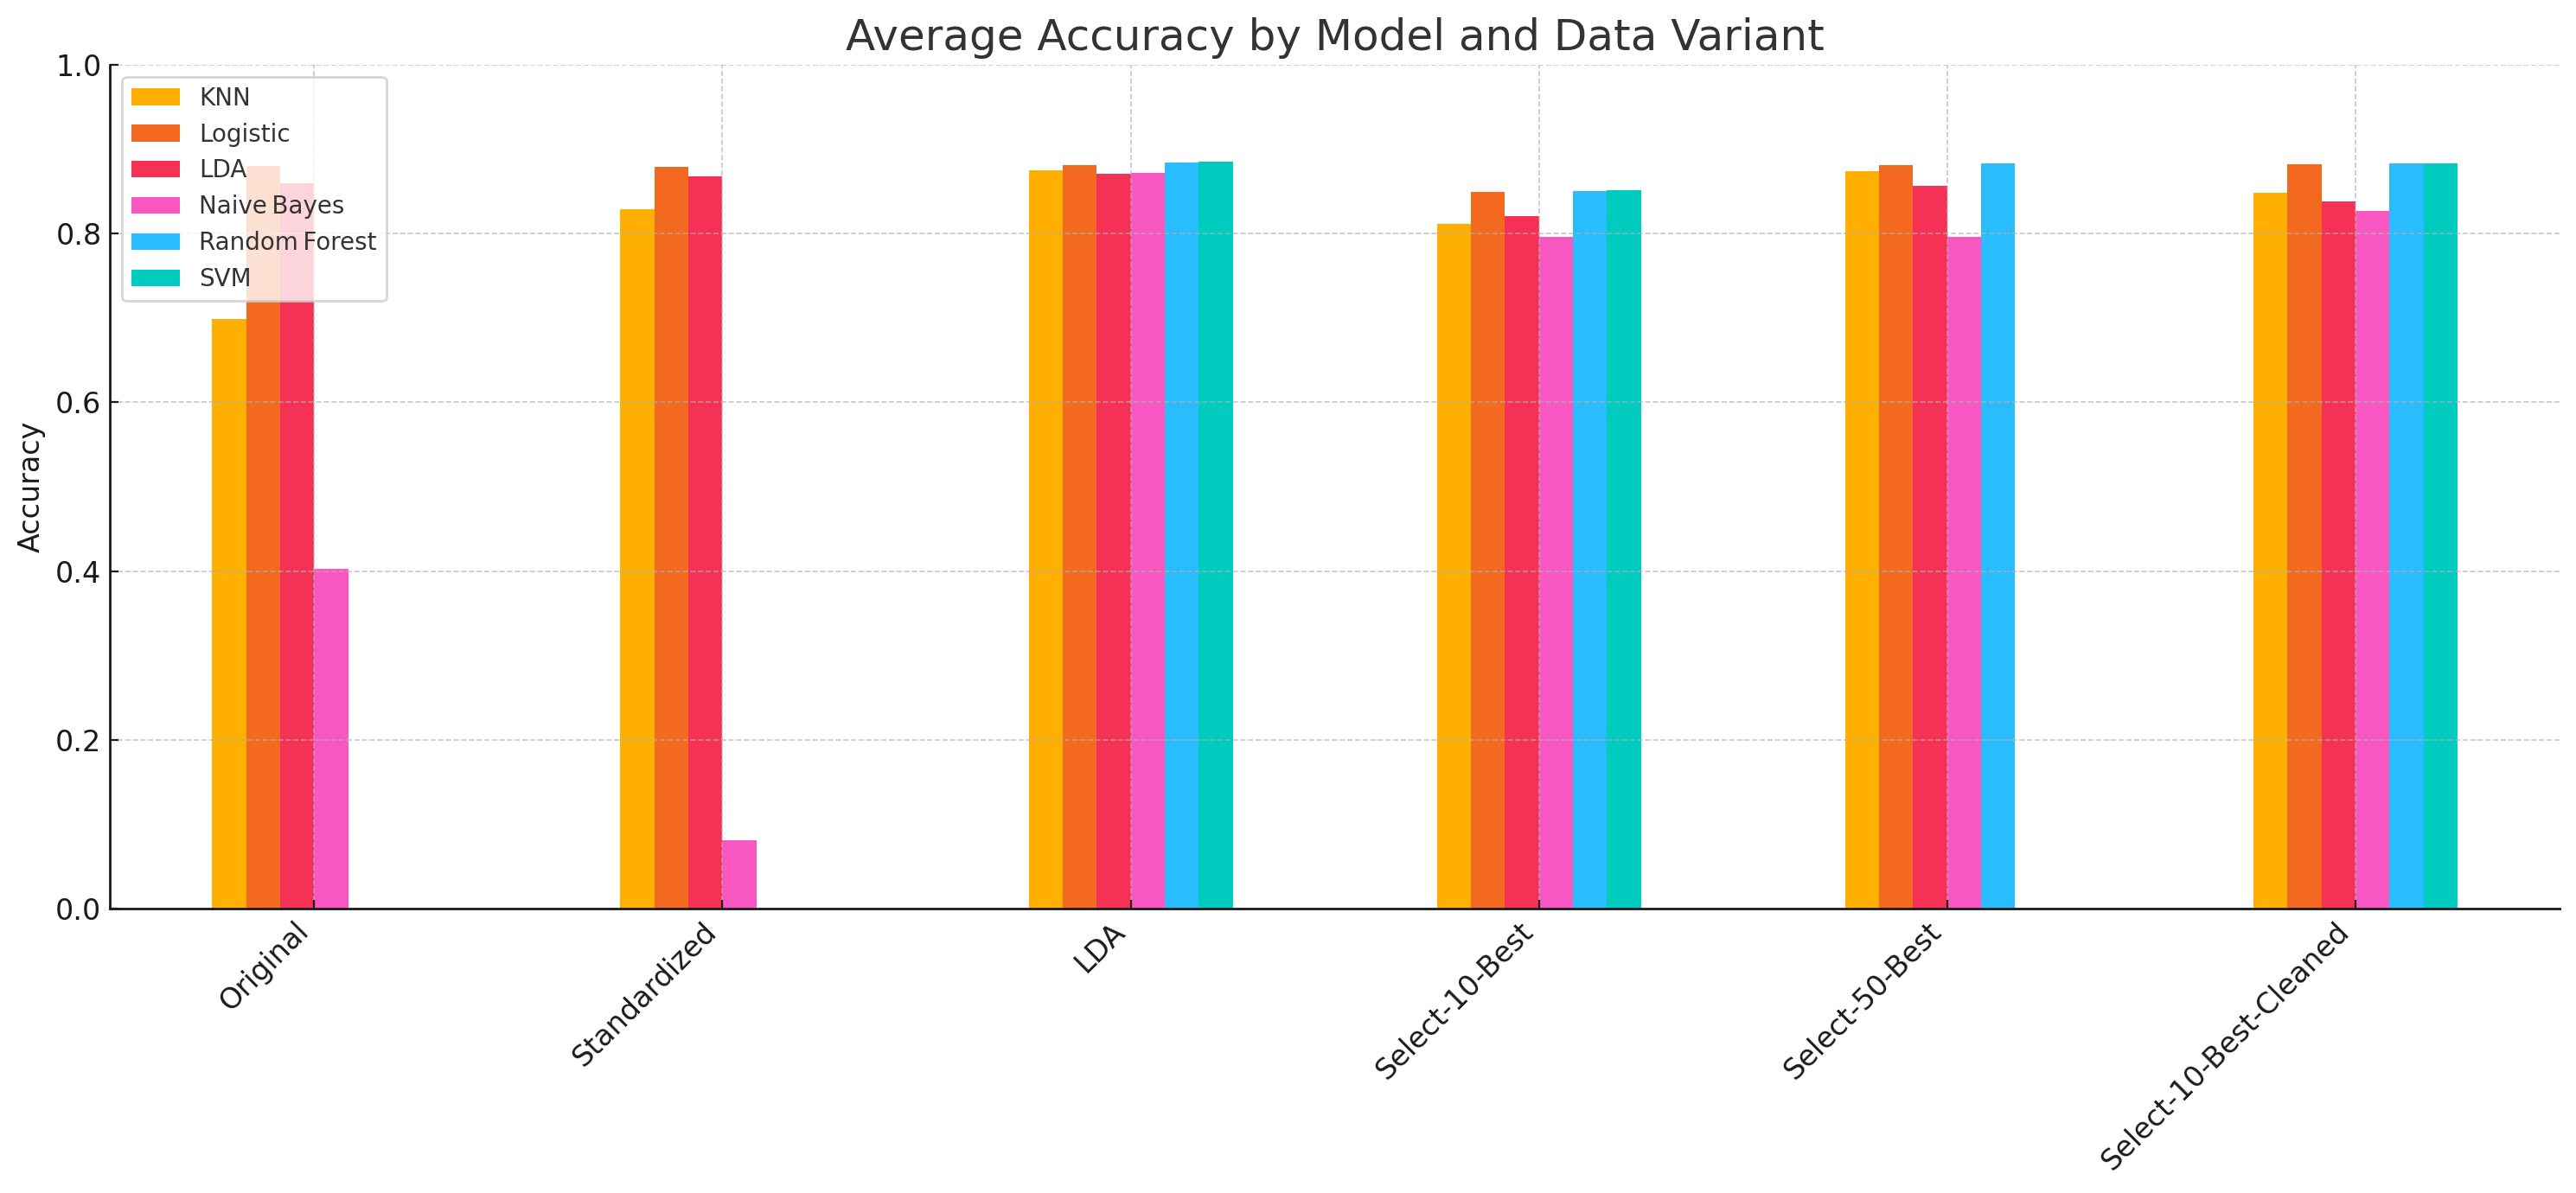
\includegraphics[width=0.8\linewidth]{cls_acc.png}
  \label{fig:10}
\end{figure}
\begin{figure}[H]
  \centering
  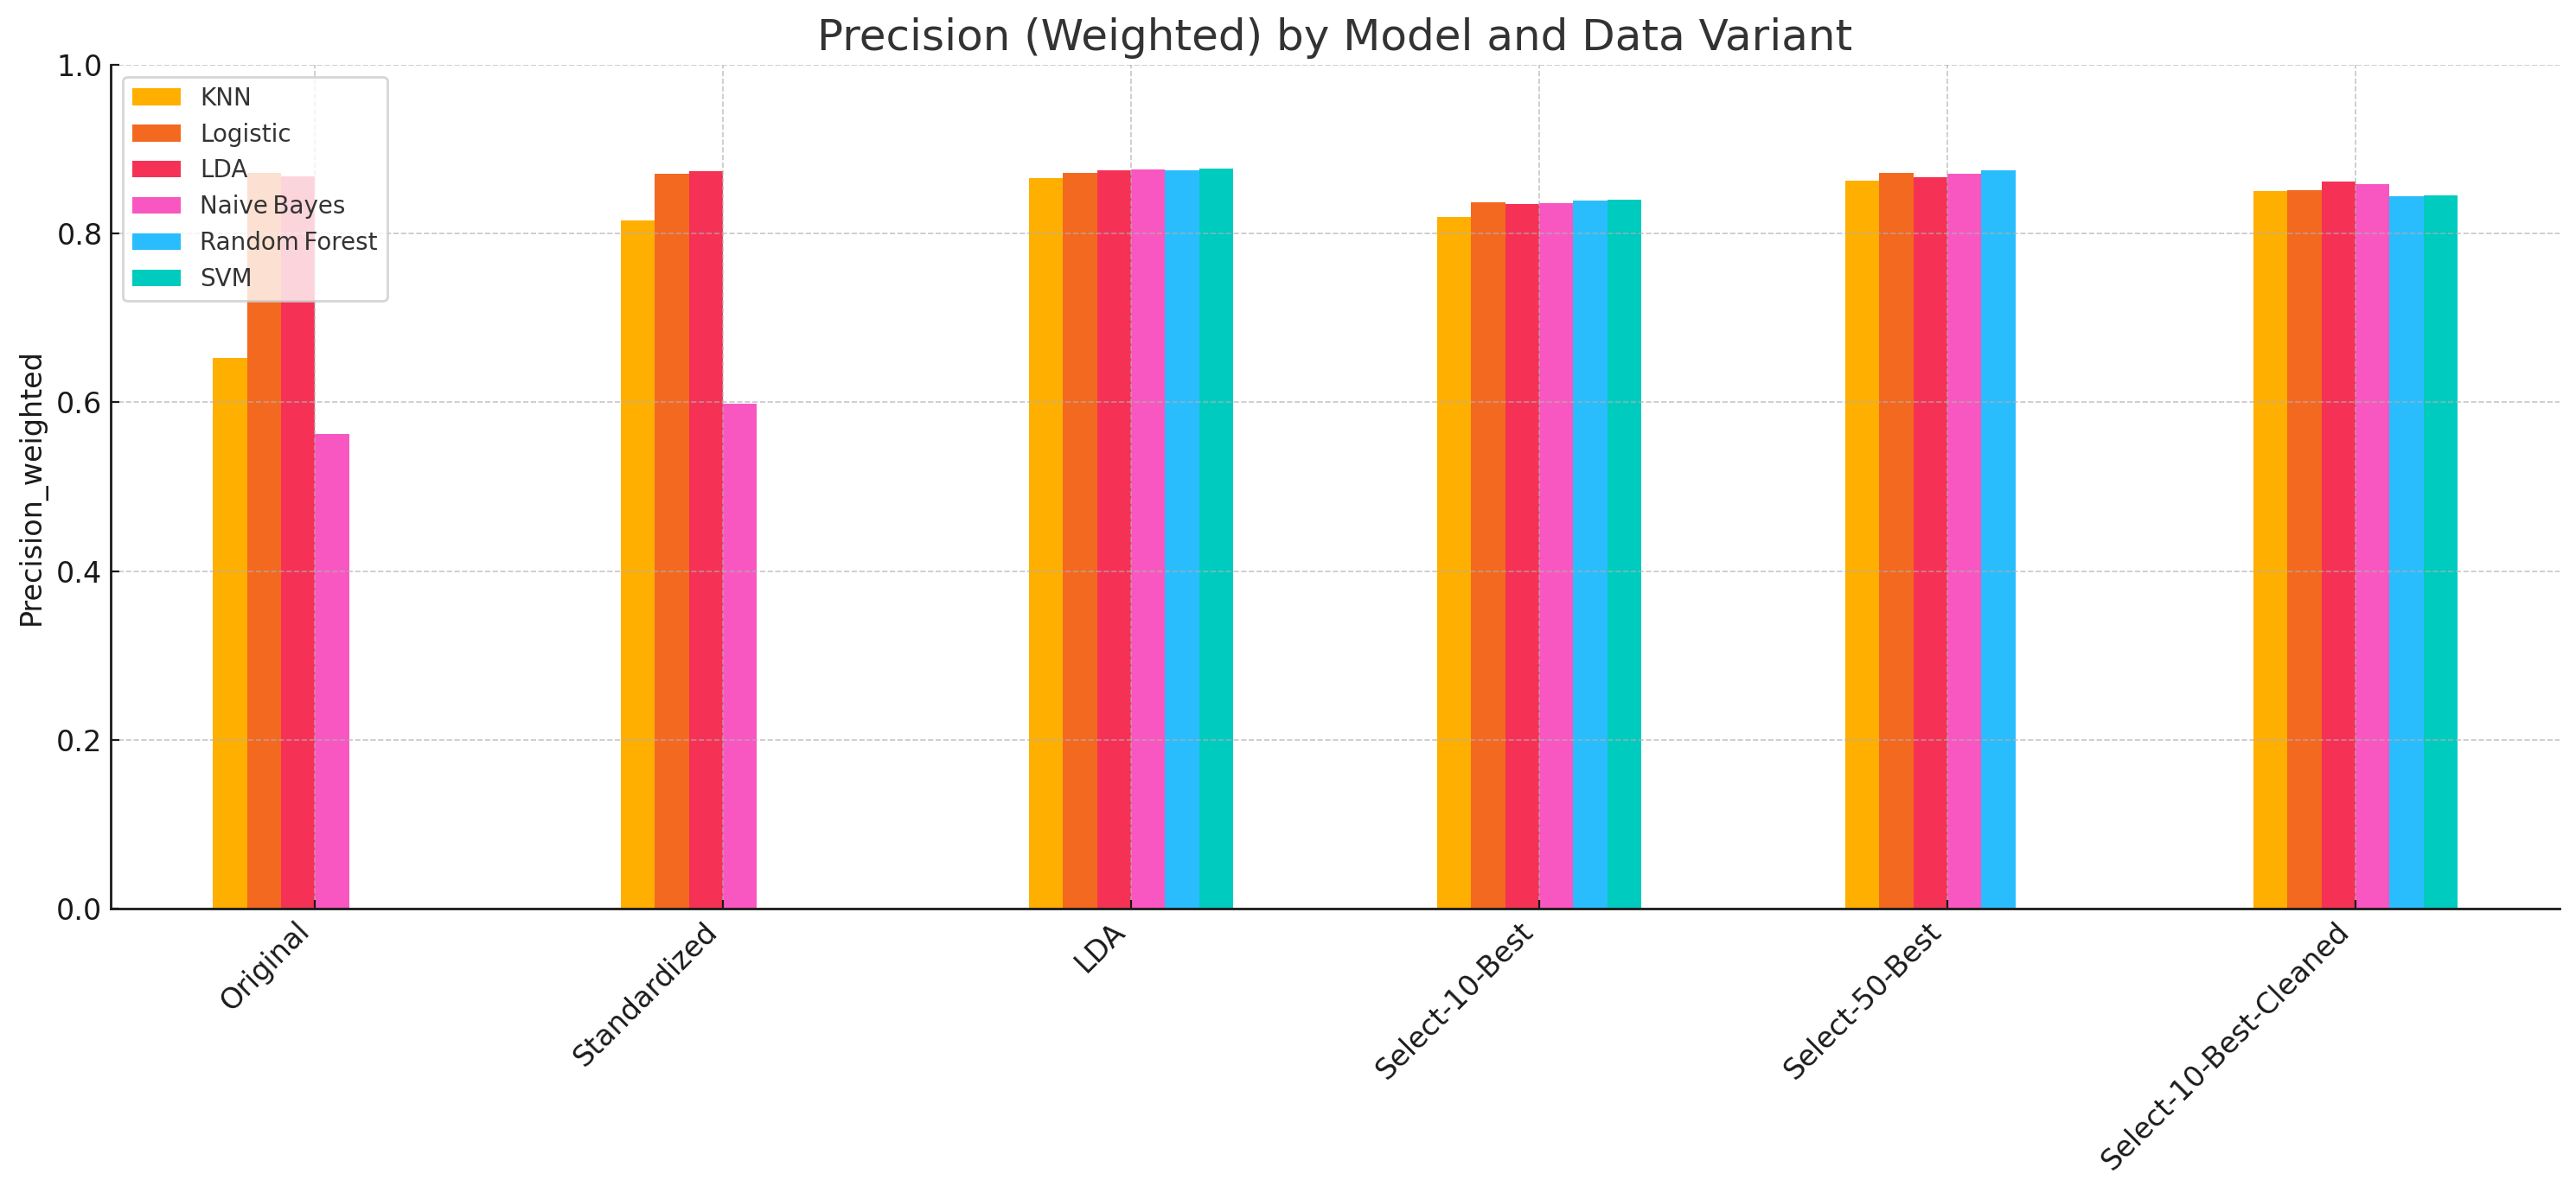
\includegraphics[width=0.8\linewidth]{cls_prec.png}
  \label{fig:11}
\end{figure}
\begin{figure}[H]
  \centering
  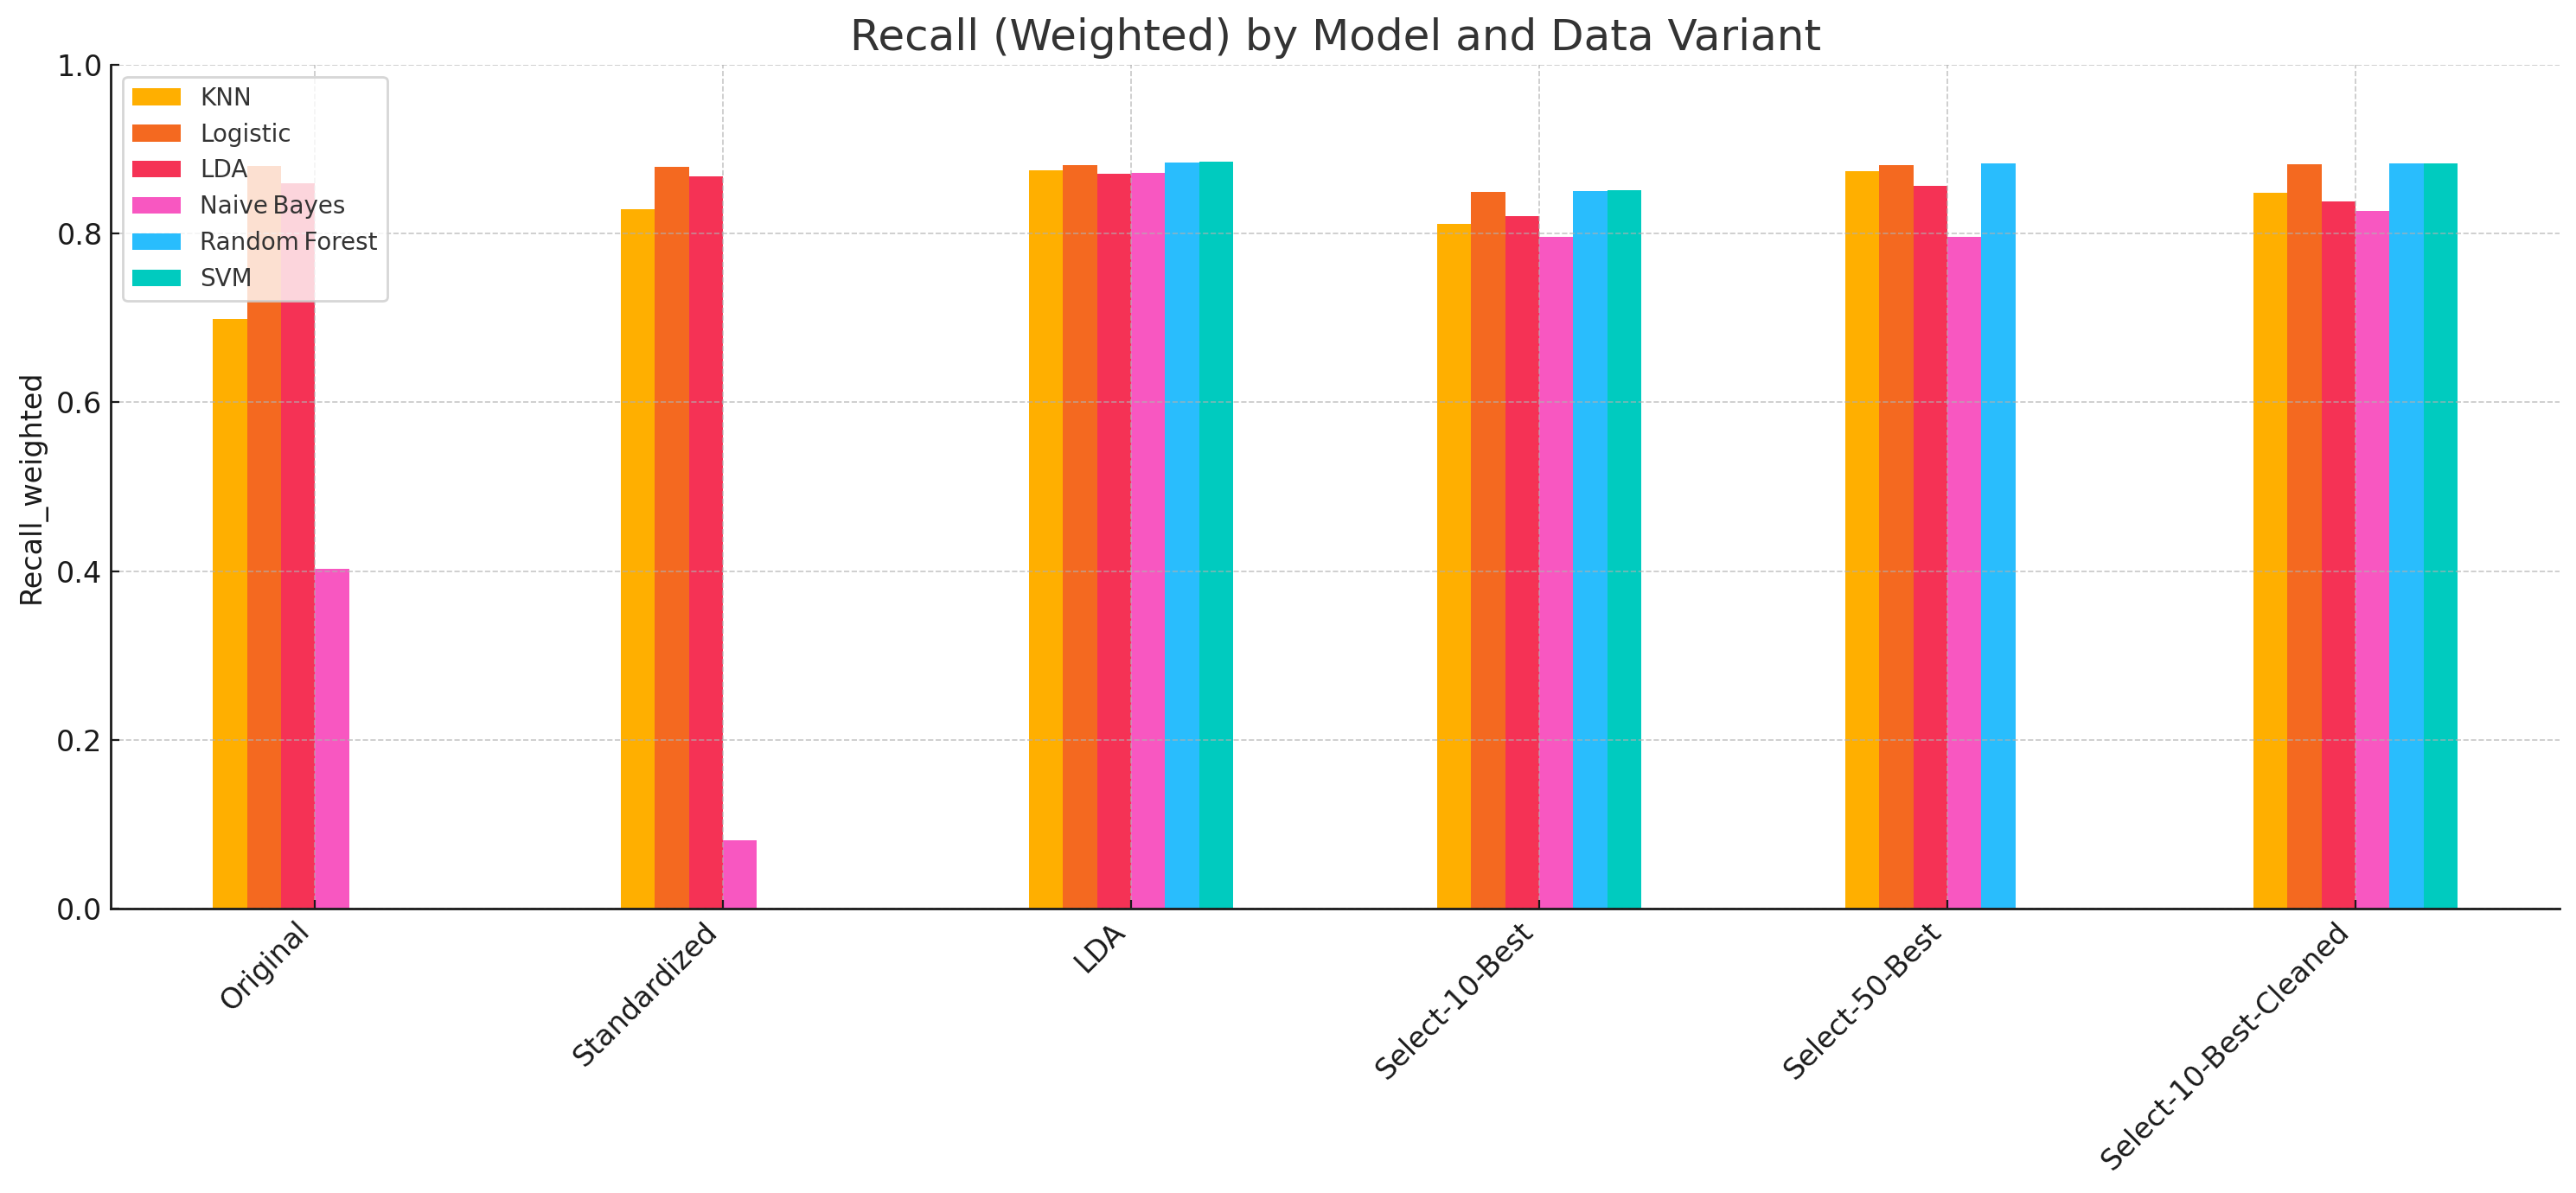
\includegraphics[width=0.8\linewidth]{cls_rec.png}
  \label{fig:12}
\end{figure}
\begin{figure}[H]
  \centering
  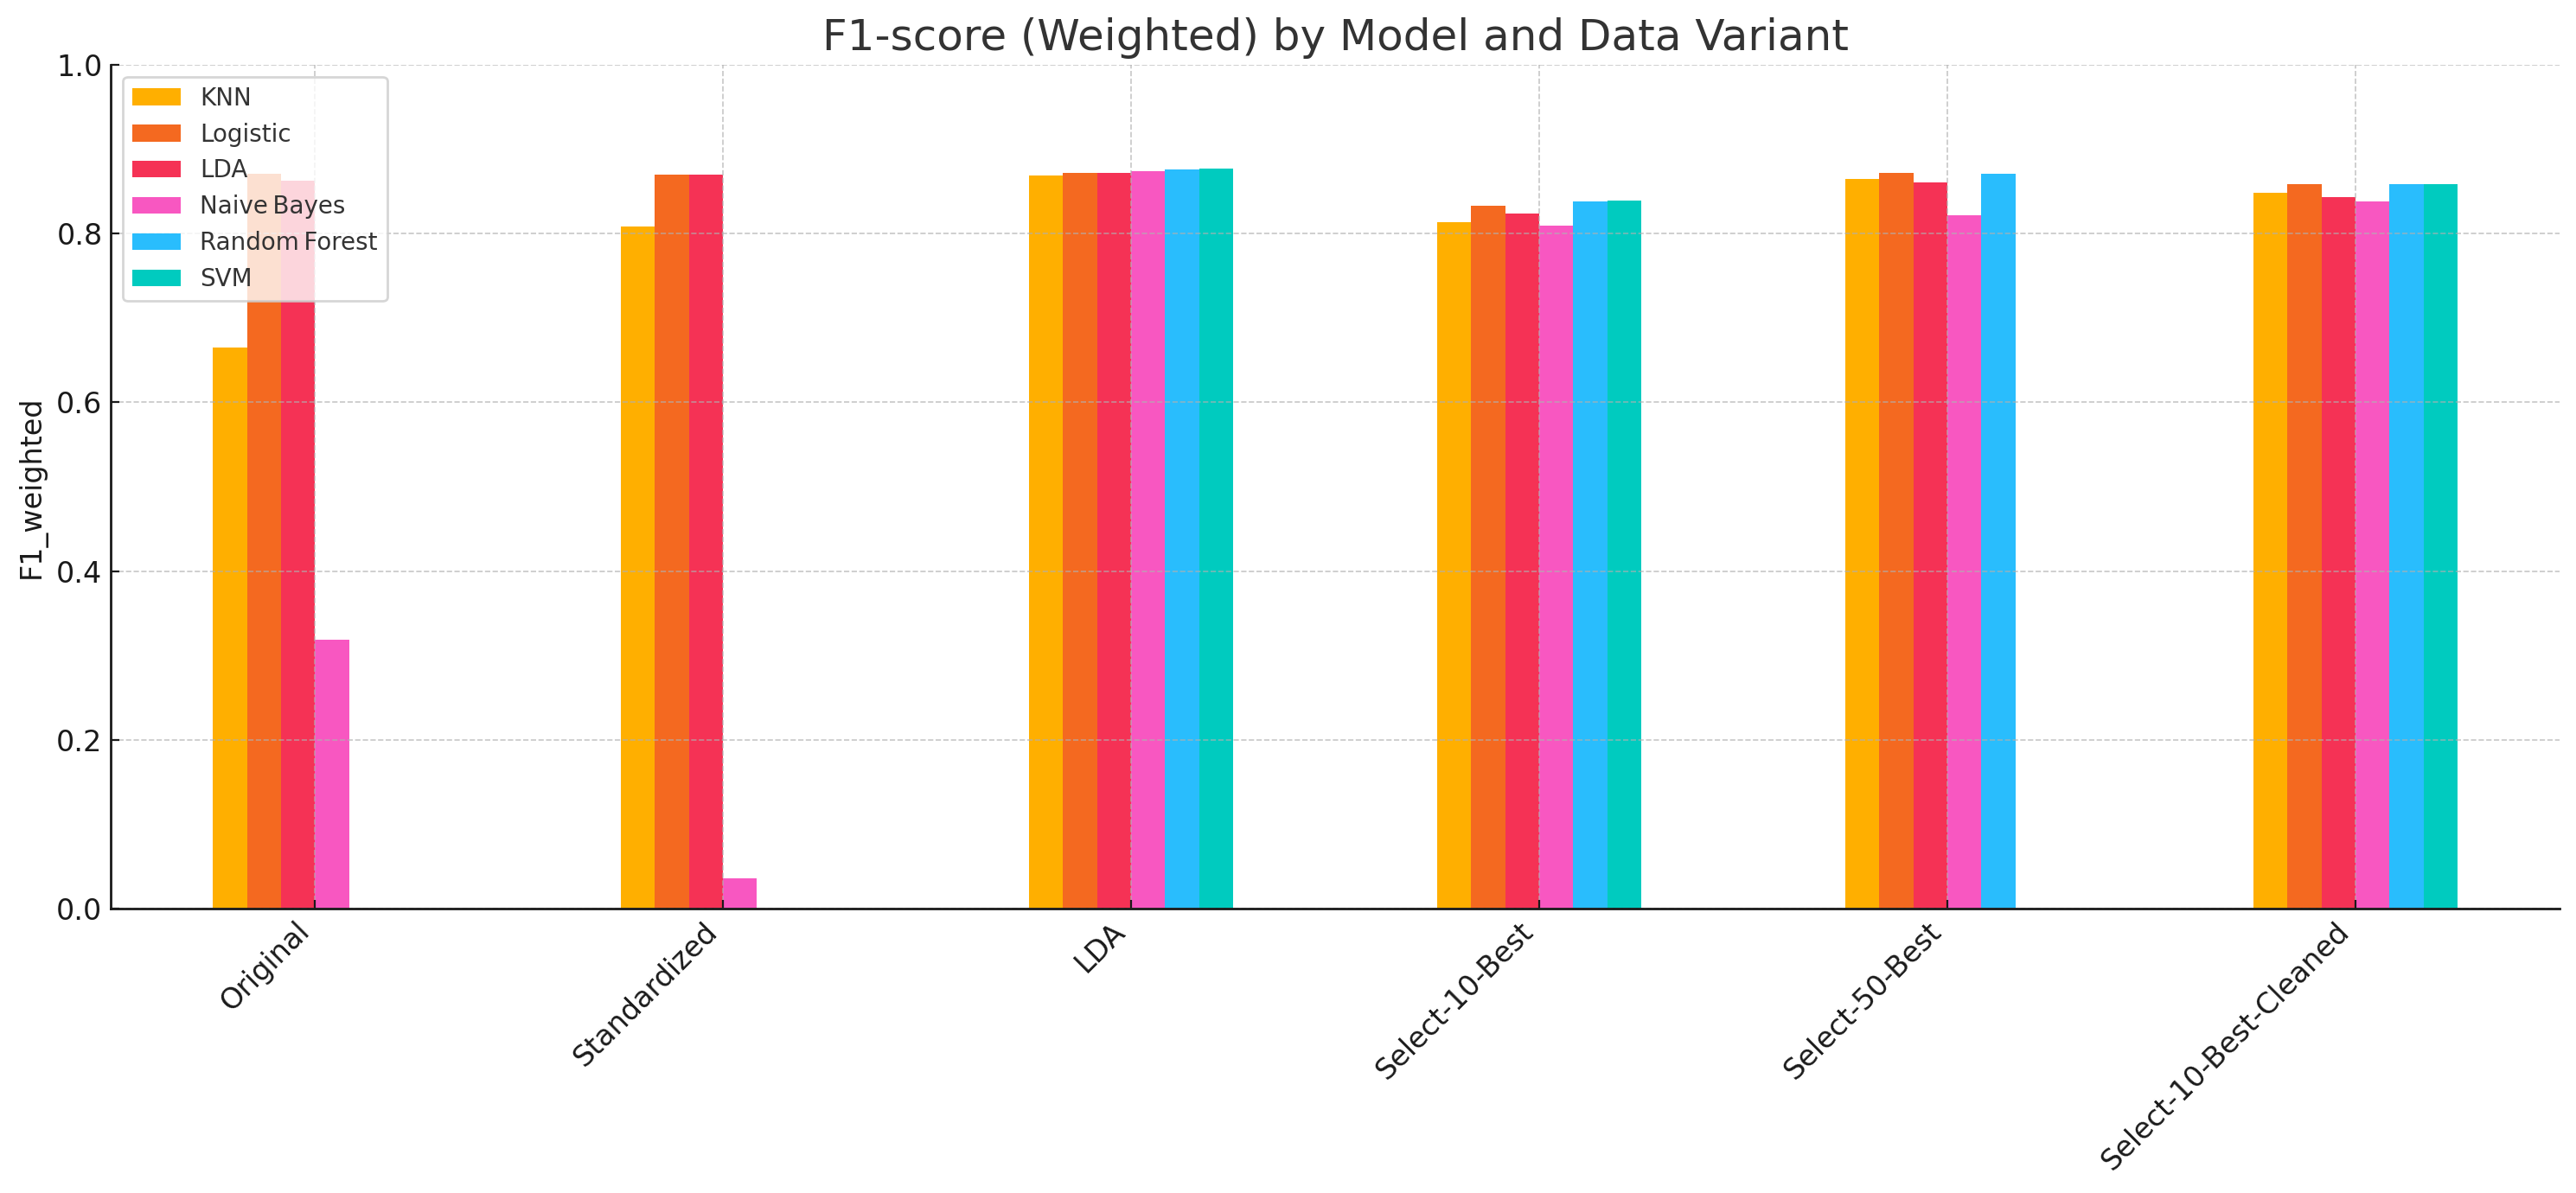
\includegraphics[width=0.8\linewidth]{cls_f1.png}
  \label{fig:14}
\end{figure}
\begin{figure}[H]
  \centering
  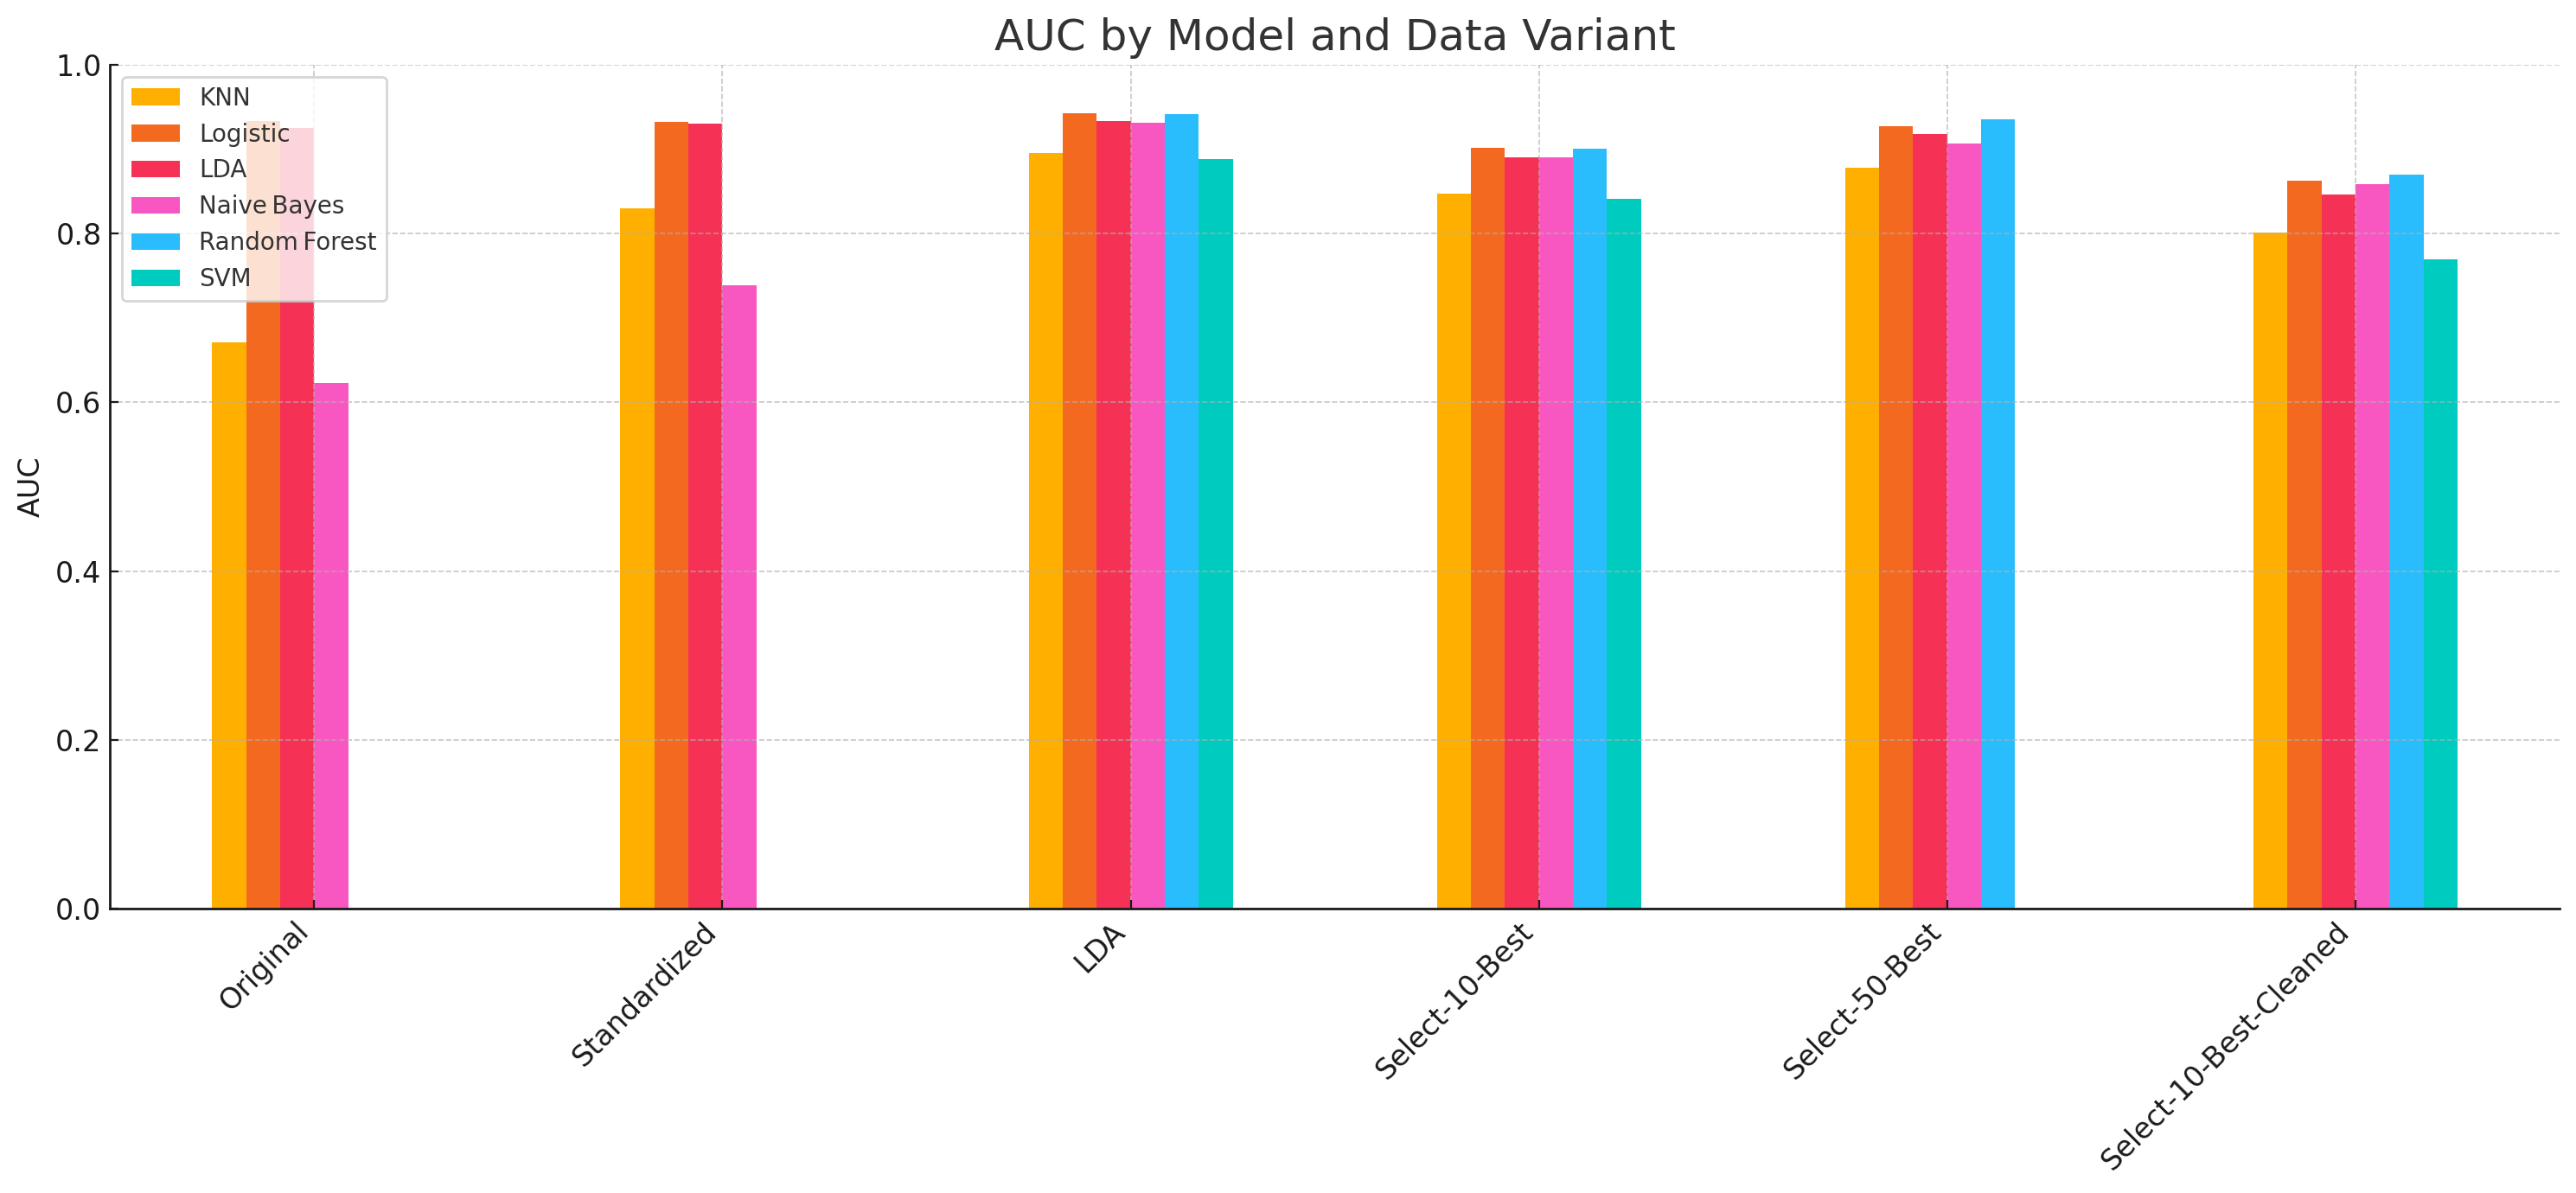
\includegraphics[width=0.8\linewidth]{cls_auc.png}
  \label{fig:80}
\end{figure}
为了更直观地看出各个模型在不同数据集下的训练效果,我同样绘制了关于Accuracy的雷达图:
\begin{figure}[H]
  \centering
  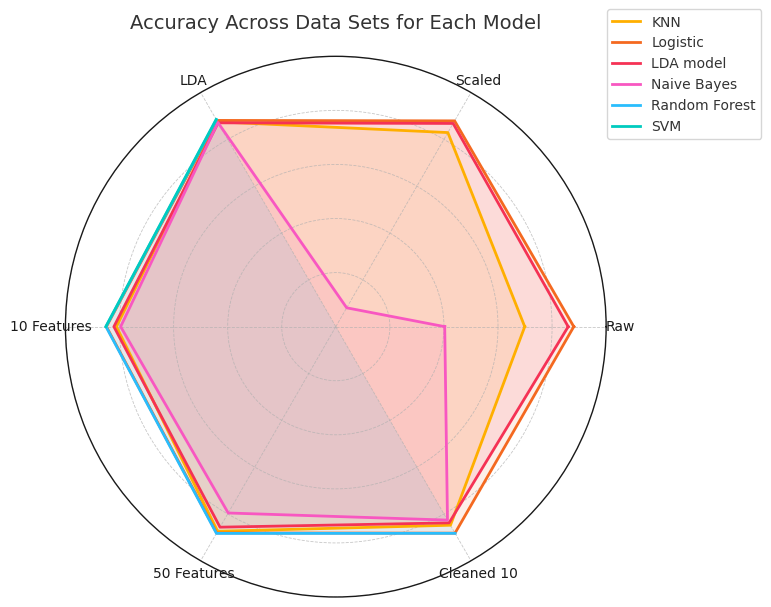
\includegraphics[width=0.7\linewidth]{radar_acc.png}
  \label{fig:81}
\end{figure}
\paragraph{分析}
\begin{itemize}
  \item 模型的选择与数据集特征
  \begin{itemize}
    \item KNN与Logistic回归:这些模型在面对标准化后的数据和LDA降维后的数据表现较好。KNN对数据的局部特征非常敏感,因此其在特征提取后能显著提高性能。Logistic回归也在特征选择后的数据集中表现出较高的精度和较低的过拟合趋势。
    \item LDA的降维效果:从实验结果看来,LDA降维技术能够显著提高分类任务的效果。与PCA不同,LDA通过利用标签信息进行降维,使得类别间的区分度最大化,从而在多个分类模型中展现了显著的性能提升。
  \end{itemize}
  \item 贝叶斯分类器的局限性
  \begin{itemize}
    \item 贝叶斯模型的低效表现:从实验结果来看,其在原始数据和标准化的数据下训练得到的性能较差,其原因可能在于贝叶斯模型假设特征之间是独立的,但在实际的旅游数据中,特征之间往往是相关的,导致贝叶斯假设不成立,性能较差。
  \end{itemize}
  \item 模型集成与鲁棒性
  \begin{itemize}
    \item 随机森林通过集成学习的方式,能够有效增强模型的鲁棒性,对特征的敏感性较低。SVM则在LDA降维后的数据集上表现尤为突出,尤其在较高维度的特征空间中,SVM通过选择适当的核函数能够提高模型的分类边界精度。
  \end{itemize}
  \item 特征选择与数据清洗的影响
  \begin{itemize}
    \item 经过实验,我们可以发现清洗数据能够显著提升一些模型的泛化能力,在特征提取后的数据集上,这些分类模型的准确性、召回率和F1分数均有所提高。说明通过剔除噪声和无关特征,能够减少模型训练中的冗余信息,从而使模型更加专注于对关键特征的学习。
  \end{itemize}
\end{itemize}


\paragraph{整体来看:}
\begin{enumerate}
  \item 随机森林在回归任务上,Logistic和随机森林在分类任务上的综合指标最优。
  \item PCA 可显著降低训练成本,且对非线性模型有较强的正向效果,但是对于随机森林等非线性模型的正向效果不佳;LDA对KNN的提升较为明显。
  \item 超参数搜索的方式能够方便我们找到合适的模型的训练参数,在实验过程中,很明显能感受到精确调节模型的超参数对于提高回归任务的表现的重要性。
  \item 数据的处理方式极大程度上地影响了模型的训练效果,回归实验中,R2负值的出现跟那些离群值密切相关,从实验的结果来看,通过Z-score的方式也没能很好地剔除掉一些异常值,后续可进行优化。
\end{enumerate}





\newpage
\appendix
\section*{附录:实验结果}
\addcontentsline{toc}{section}{附录:实验结果}
\section{回归任务结果}
\subsection{线性模型}
\subsubsection*{原始数据:}
  \begin{figure}[H]
  \centering
  \makebox[\textwidth][c]{%
    % 表格部分
    \parbox{0.48\textwidth}{%
      \centering
      \captionof{table}{线性模型原始数据训练下五折评估指标}
      \begin{tabular}{lccc}
          \toprule
          折数 & MSE & MAE & R2 \\ \midrule
          Fold 1 & 336.8344 & 5.7650 & 0.1689 \\
          Fold 2 & 9770.1011 & 10.4300 & 28.7898 \\
          Fold 3 & 336.3178 & 5.4946 & 0.0355 \\
          Fold 4 & 346.0066 & 5.2283 & 0.0926 \\
          Fold 5 & 553.5520 & 6.1636 & 0.0664 \\
          Average & 2268.5624 & 6.6163 & -5.6853 \\
          Best & 336.8344 & 5.7650 & 0.1689 \\
          \bottomrule
      \end{tabular}
    }
    \hfill
    % 图像部分
    \parbox{0.48\textwidth}{%
      \centering
      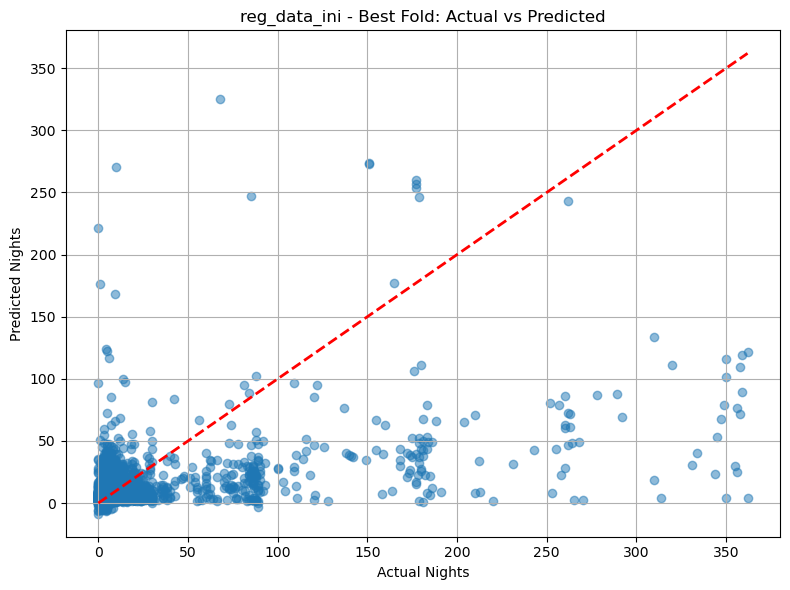
\includegraphics[width=\linewidth]{reg_lr_ini.png}
      \captionof{figure}{Actual Nights vs Predicted Nights}
      \label{fig:1-1}
    }
  }
  \end{figure}
\subsubsection*{标准化数据:}
  \begin{figure}[H]
  \centering
  \makebox[\textwidth][c]{%
    % 表格部分
    \parbox{0.48\textwidth}{%
      \centering
      \captionof{table}{线性模型标准化数据训练下五折评估指标}
      \begin{tabular}{lccc}
          \toprule
          折数 & MSE & MAE & R2 \\ \midrule
          Fold 1 & 263.3822 & 7.4275 & 0.3502 \\
          Fold 2 & 5990.6823 & 11.3312 & -17.2660 \\
          Fold 3 & 278.0367 & 6.4655 & 0.2026 \\
          Fold 4 & 268.0578 & 6.3568 & 0.2971 \\
          Fold 5 & 377.1054 & 6.7491 & 0.3640 \\
          Average & 1435.4529 & 7.6660 & -3.2104 \\
          Best & 377.1054 & 6.7491 & 0.3640 \\
          \bottomrule
      \end{tabular}
    }
    \hfill
    % 图像部分
    \parbox{0.48\textwidth}{%
      \centering
      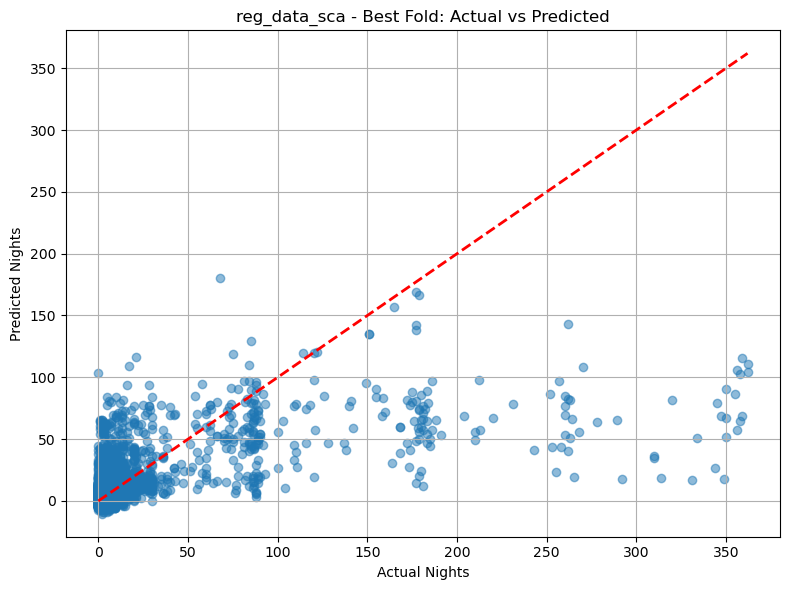
\includegraphics[width=\linewidth]{reg_lr_sca.png}
      \captionof{figure}{Actual Nights vs Predicted Nights}
      \label{fig:1-2}
    }
  }
  \end{figure}

\subsubsection*{PCA数据:}
  \begin{figure}[H]
  \centering
  \makebox[\textwidth][c]{%
    % 表格部分
    \parbox{0.48\textwidth}{%
      \centering
      \captionof{table}{线性模型PCA数据训练下五折评估指标}
      \begin{tabular}{lccc}
          \toprule
          折数 & MSE & MAE & R2 \\ \midrule
          Fold 1 & 312.1421 & 7.1290 & 0.2298 \\
          Fold 2 & 3560.3123 & 11.3488 & -9.8557 \\
          Fold 3 & 307.5704 & 6.1773 & 0.1180 \\
          Fold 4 & 341.9268 & 6.1012 & 0.1033 \\
          Fold 5 & 524.3376 & 7.0610 & 0.1157 \\
          Average & 1009.2578 & 7.5635 & -1.8578 \\
          Best & 312.1421 & 7.1290 & 0.2298 \\
          \bottomrule
      \end{tabular}
    }
    \hfill
    % 图像部分
    \parbox{0.48\textwidth}{%
      \centering
      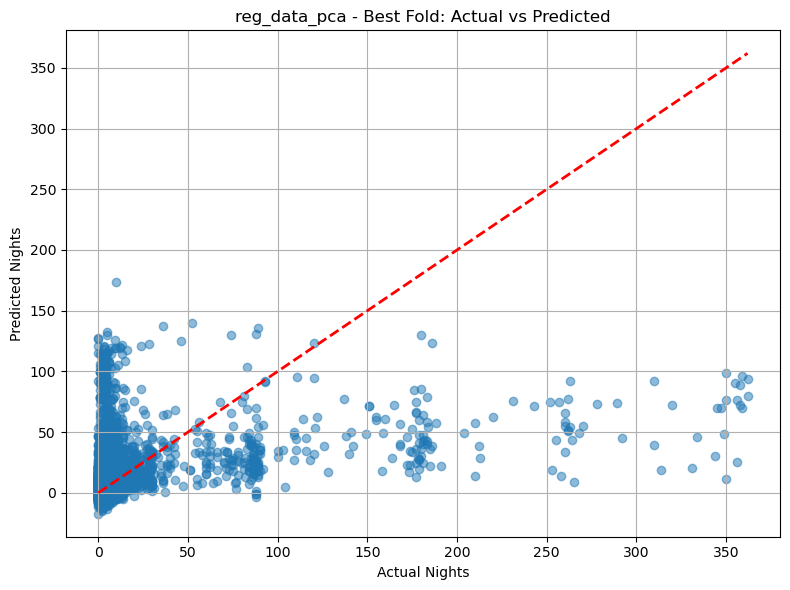
\includegraphics[width=\linewidth]{reg_lr_pca.png}
      \captionof{figure}{Actual Nights vs Predicted Nights}
      \label{fig:1-3}
    }
  }
  \end{figure}

\subsubsection*{10项特征提取数据:}
  \begin{figure}[H]
  \centering
  \makebox[\textwidth][c]{%
    % 表格部分
    \parbox{0.48\textwidth}{%
      \centering
      \captionof{table}{线性模型10项特征提取数据训练下五折评估指标}
      \begin{tabular}{lccc}
          \toprule
          折数 & MSE & MAE & R2 \\ \midrule
          Fold 1 & 263.3822 & 7.4275 & 0.3502 \\
          Fold 2 & 5990.6823 & 11.3312 & -17.2660 \\
          Fold 3 & 278.0367 & 6.4655 & 0.2026 \\
          Fold 4 & 268.0578 & 6.3568 & 0.2971 \\
          Fold 5 & 377.1054 & 6.7491 & 0.3640 \\
          Average & 1435.4529 & 7.6660 & -3.2104 \\
          Best & 377.1054 & 6.7491 & 0.3640 \\
          \bottomrule
      \end{tabular}
    }
    \hfill
    % 图像部分
    \parbox{0.48\textwidth}{%
      \centering
      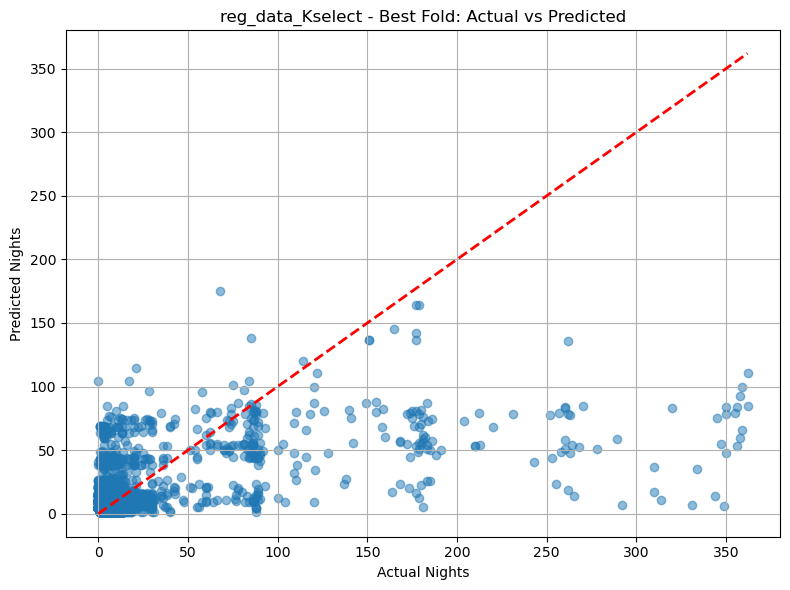
\includegraphics[width=\linewidth]{reg_lr_10s.png}
      \captionof{figure}{Actual Nights vs Predicted Nights}
      \label{fig:1-4}
    }
  }
  \end{figure}

\subsubsection*{50项特征提取数据:}
  \begin{figure}[H]
  \centering
  \makebox[\textwidth][c]{%
    % 表格部分
    \parbox{0.48\textwidth}{%
      \centering
      \captionof{table}{线性模型50项特征提取数据训练下五折评估指标}
      \begin{tabular}{lccc}
          \toprule
          折数 & MSE & MAE & R2 \\ \midrule
          Fold 1 & 255.0999 & 6.6487 & 0.3706 \\
          Fold 2 & 4664.2164 & 9.6479 & -13.2216 \\
          Fold 3 & 278.7787 & 5.9347 & 0.2005 \\
          Fold 4 & 269.4189 & 6.0050 & 0.2935 \\
          Fold 5 & 382.4730 & 6.5599 & 0.3549 \\
          Average & 1169.9974 & 6.9592 & -2.4004 \\
          Best & 255.0999 & 6.6487 & 0.3706 \\
          \bottomrule
      \end{tabular}
    }
    \hfill
    % 图像部分
    \parbox{0.48\textwidth}{%
      \centering
      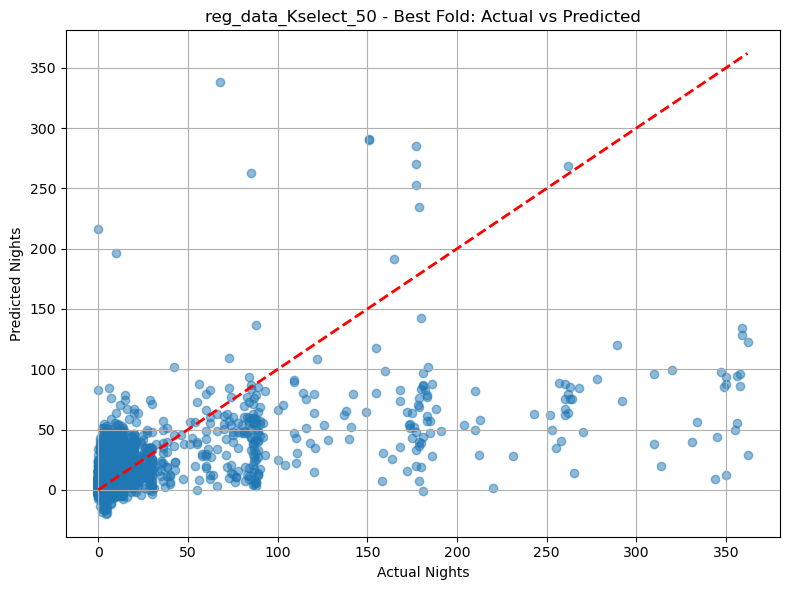
\includegraphics[width=\linewidth]{reg_lr_50s.png}
      \captionof{figure}{Actual Nights vs Predicted Nights}
      \label{fig:1-5}
    }
  }
  \end{figure}

\subsubsection*{清洗后的10项特征提取数据:}
  \begin{figure}[H]
  \centering
  \makebox[\textwidth][c]{%
    % 表格部分
    \parbox{0.48\textwidth}{%
      \centering
      \captionof{table}{线性模型清洗后的10项特征提取数据训练下五折评估指标}
      \begin{tabular}{lccc}
          \toprule
          折数 & MSE & MAE & R2 \\ \midrule
          Fold 1 & 18.3113 & 2.2221 & 0.0742 \\
          Fold 2 & 22.2196 & 2.4794 & 0.0018 \\
          Fold 3 & 18.5999 & 2.3345 & 0.0931 \\
          Fold 4 & 17.2894 & 2.1478 & 0.0835 \\
          Fold 5 & 13.5112 & 2.1708 & 0.0798 \\
          Average & 17.9863 & 2.2709 & 0.0665 \\
          Best & 18.5999 & 2.3345 & 0.0931 \\
          \bottomrule
      \end{tabular}
    }
    \hfill
    % 图像部分
    \parbox{0.48\textwidth}{%
      \centering
      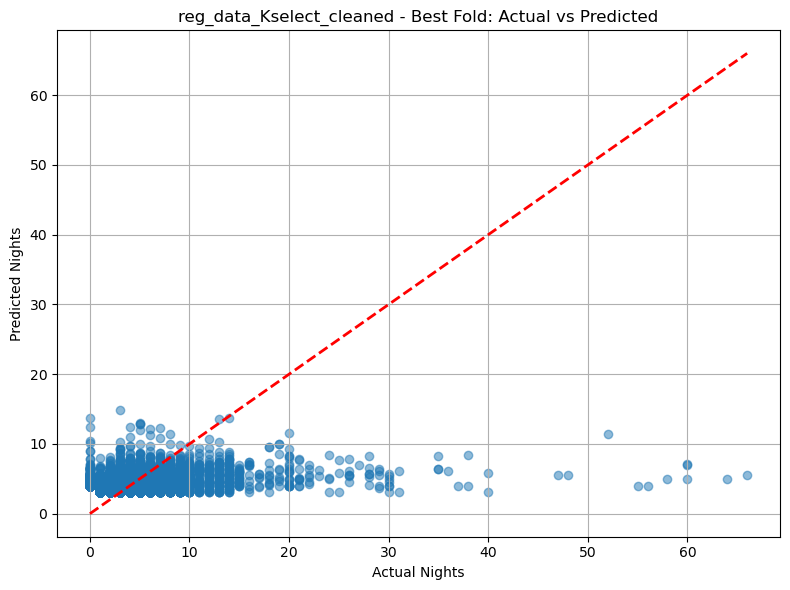
\includegraphics[width=\linewidth]{reg_lr_10sc.png}
      \captionof{figure}{Actual Nights vs Predicted Nights}
      \label{fig:1-6}
    }
  }
  \end{figure}

\subsection{Lasso回归模型}
\subsubsection*{原始数据:}
  \begin{figure}[H]
  \centering
  \makebox[\textwidth][c]{%
    % 表格部分
    \parbox{0.48\textwidth}{%
      \centering
      \captionof{table}{Lasso回归模型原始数据训练下五折评估指标}
      \begin{tabular}{lccc}
          \toprule
          折数 & MSE & MAE & R2 \\ \midrule
          Fold 1 & 257.2531 & 6.3735 & 0.3653 \\
          Fold 2 & 6008.5252 & 10.9164 & -17.3205 \\
          Fold 3 & 274.7042 & 6.1136 & 0.2122 \\
          Fold 4 & 284.7410 & 6.1634 & 0.2533 \\
          Fold 5 & 377.8516 & 6.5836 & 0.3627 \\
          Average & 1440.6150 & 7.2301 & -3.2254 \\
          Best & 257.2531 & 6.3735 & 0.3653 \\
          \bottomrule
      \end{tabular}
    }
    \hfill
    % 图像部分
    \parbox{0.48\textwidth}{%
      \centering
      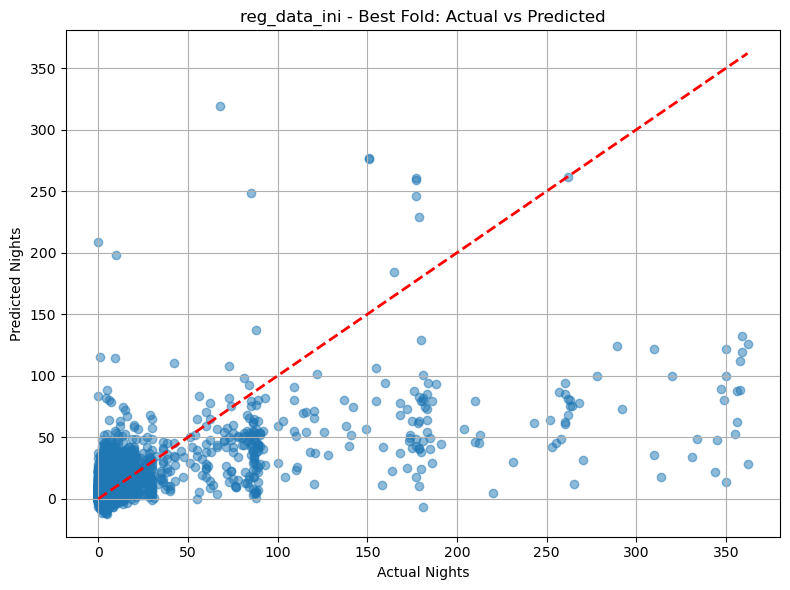
\includegraphics[width=\linewidth]{reg_la_ini.png}
      \captionof{figure}{Actual Nights vs Predicted Nights}
      \label{fig:2-1}
    }
  }
  \end{figure}
\subsubsection*{标准化数据:}
  \begin{figure}[H]
  \centering
  \makebox[\textwidth][c]{%
    % 表格部分
    \parbox{0.48\textwidth}{%
      \centering
      \captionof{table}{Lasso回归模型标准化数据训练下五折评估指标}
      \begin{tabular}{lccc}
          \toprule
          折数 & MSE & MAE & R2 \\ \midrule
          Fold 1 & 255.2289 & 6.7233 & 0.3703 \\
          Fold 2 & 4454.9847 & 9.6282 & -12.5836 \\
          Fold 3 & 348.7290 & 5.5576 & -0.0001 \\
          Fold 4 & 314.9393 & 4.8643 & 0.1741 \\
          Fold 5 & 594.3588 & 6.4180 & -0.0024 \\
          Average & 1193.6481 & 6.6383 & -2.4083 \\
          Best & 255.2289 & 6.7233 & 0.3703 \\
          \bottomrule
      \end{tabular}
    }
    \hfill
    % 图像部分
    \parbox{0.48\textwidth}{%
      \centering
      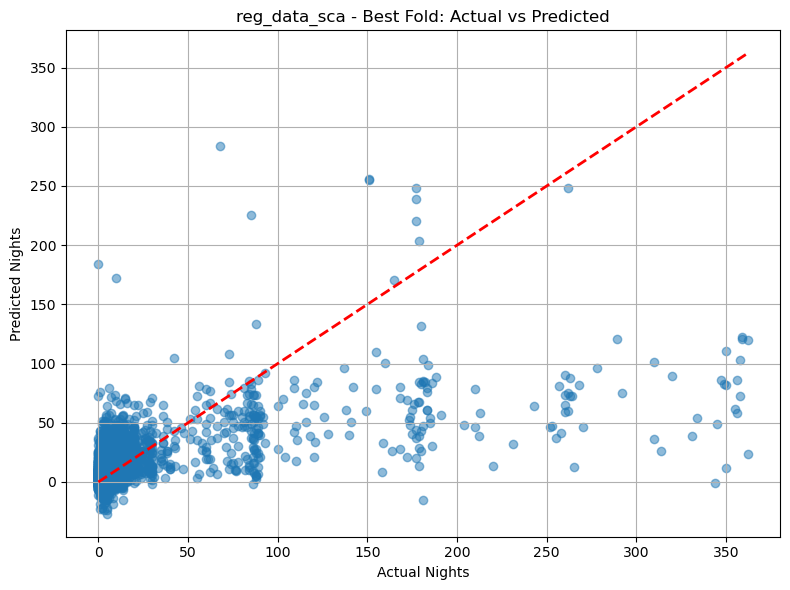
\includegraphics[width=\linewidth]{reg_la_sca.png}
      \captionof{figure}{Actual Nights vs Predicted Nights}
      \label{fig:2-2}
    }
  }
  \end{figure}

\subsubsection*{PCA数据:}
  \begin{figure}[H]
  \centering
  \makebox[\textwidth][c]{%
    % 表格部分
    \parbox{0.48\textwidth}{%
      \centering
      \captionof{table}{Lasso回归模型PCA数据训练下五折评估指标}
      \begin{tabular}{lccc}
          \toprule
          折数 & MSE & MAE & R2 \\ \midrule
          Fold 1 & 312.6796 & 6.9356 & 0.2285 \\
          Fold 2 & 3500.8981 & 11.2568 & -9.6745 \\
          Fold 3 & 343.0862 & 5.3790 & 0.0161 \\
          Fold 4 & 341.6980 & 6.0224 & 0.1039 \\
          Fold 5 & 589.7213 & 6.2965 & 0.0054 \\
          Average & 1017.6166 & 7.1781 & -1.8641 \\
          Best & 312.6796 & 6.9356 & 0.2285 \\
          \bottomrule
      \end{tabular}
    }
    \hfill
    % 图像部分
    \parbox{0.48\textwidth}{%
      \centering
      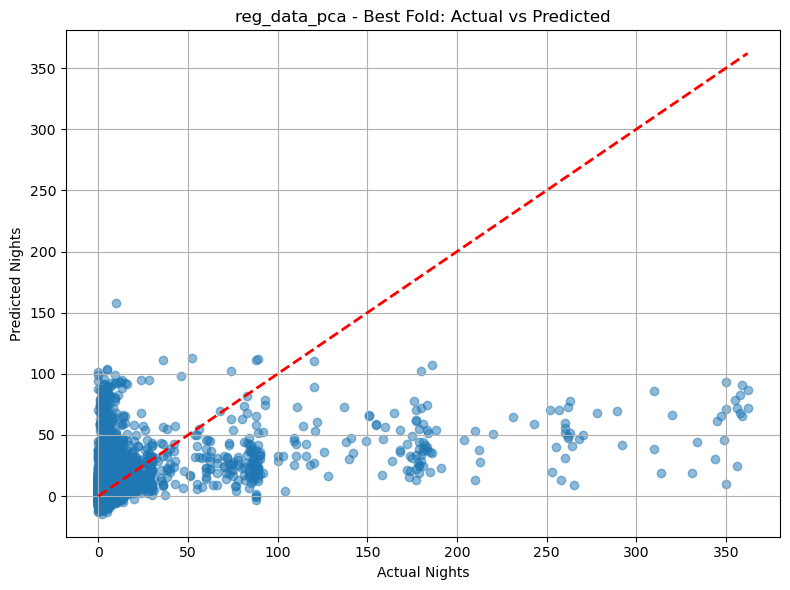
\includegraphics[width=\linewidth]{reg_la_pca.png}
      \captionof{figure}{Actual Nights vs Predicted Nights}
      \label{fig:2-3}
    }
  }
  \end{figure}

\subsubsection*{10项特征提取数据:}
  \begin{figure}[H]
  \centering
  \makebox[\textwidth][c]{%
    % 表格部分
    \parbox{0.48\textwidth}{%
      \centering
      \captionof{table}{Lasso回归模型10项特征提取数据训练下五折评估指标}
      \begin{tabular}{lccc}
          \toprule
          折数 & MSE & MAE & R2 \\ \midrule
          Fold 1 & 278.8121 & 6.1926 & 0.3121 \\
          Fold 2 & 1873.2836 & 7.9888 & -4.7118 \\
          Fold 3 & 348.7290 & 5.5576 & -0.0001 \\
          Fold 4 & 284.5554 & 5.5936 & 0.2538 \\
          Fold 5 & 594.3588 & 6.4180 & -0.0024 \\
          Average & 675.9478 & 6.3501 & -0.8297 \\
          Best & 278.8121 & 6.1926 & 0.3121 \\
          \bottomrule
      \end{tabular}
    }
    \hfill
    % 图像部分
    \parbox{0.48\textwidth}{%
      \centering
      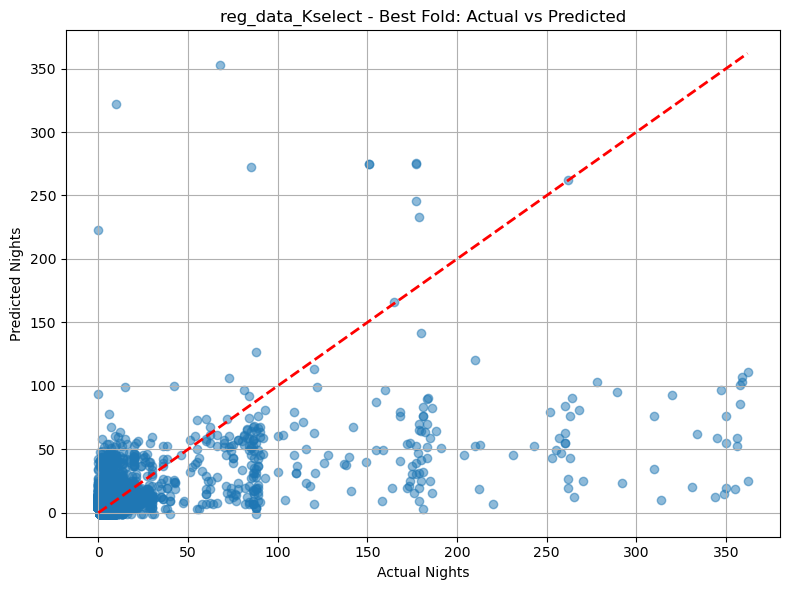
\includegraphics[width=\linewidth]{reg_la_10s.png}
      \captionof{figure}{Actual Nights vs Predicted Nights}
      \label{fig:2-4}
    }
  }
  \end{figure}

\subsubsection*{50项特征提取数据:}
  \begin{figure}[H]
  \centering
  \makebox[\textwidth][c]{%
    % 表格部分
    \parbox{0.48\textwidth}{%
      \centering
      \captionof{table}{Lasso回归模型50项特征提取数据训练下五折评估指标}
      \begin{tabular}{lccc}
          \toprule
          折数 & MSE & MAE & R2 \\ \midrule
          Fold 1 & 255.0154 & 6.4352 & 0.3708 \\
          Fold 2 & 4084.1204 & 9.2168 & -11.4528 \\
          Fold 3 & 348.7290 & 5.5576 & -0.0001 \\
          Fold 4 & 280.7685 & 5.8259 & 0.2637 \\
          Fold 5 & 594.3588 & 6.4180 & -0.0024 \\
          Average & 1112.5984 & 6.6907 & -2.1642 \\
          Best & 255.0154 & 6.4352 & 0.3708 \\
          \bottomrule
      \end{tabular}
    }
    \hfill
    % 图像部分
    \parbox{0.48\textwidth}{%
      \centering
      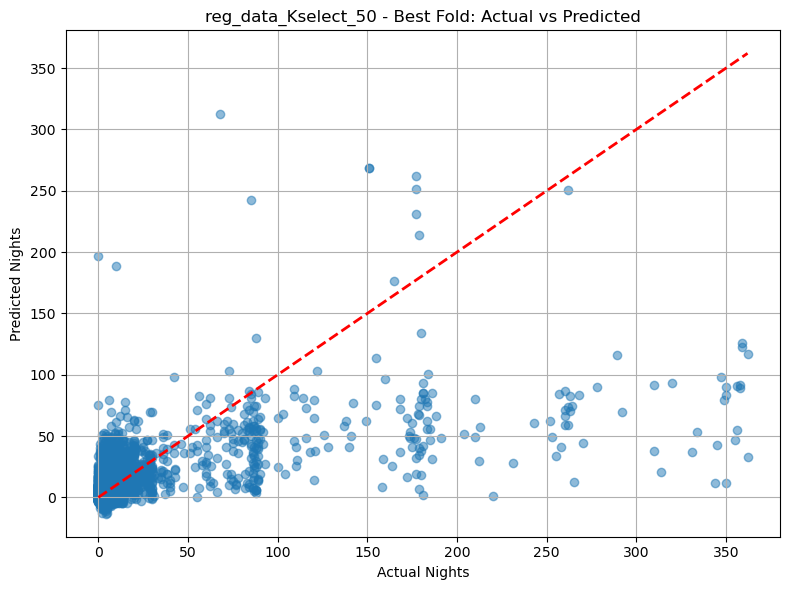
\includegraphics[width=\linewidth]{reg_la_50s.png}
      \captionof{figure}{Actual Nights vs Predicted Nights}
      \label{fig:2-5}
    }
  }
  \end{figure}

\subsubsection*{清洗后的10项特征提取数据:}
  \begin{figure}[H]
  \centering
  \makebox[\textwidth][c]{%
    % 表格部分
    \parbox{0.48\textwidth}{%
      \centering
      \captionof{table}{Lasso回归模型清洗后的10项特征提取数据训练下五折评估指标}
      \begin{tabular}{lccc}
          \toprule
          折数 & MSE & MAE & R2 \\ \midrule
          Fold 1 & 18.3168 & 2.2185 & 0.0739 \\
          Fold 2 & 22.0965 & 2.4660 & 0.0073 \\
          Fold 3 & 18.6227 & 2.3356 & 0.0920 \\
          Fold 4 & 17.3055 & 2.1490 & 0.0826 \\
          Fold 5 & 13.5125 & 2.1702 & 0.0797 \\
          Average & 17.9708 & 2.2679 & 0.0671 \\
          Best & 18.6227 & 2.3356 & 0.0920 \\
          \bottomrule
      \end{tabular}
    }
    \hfill
    % 图像部分
    \parbox{0.48\textwidth}{%
      \centering
      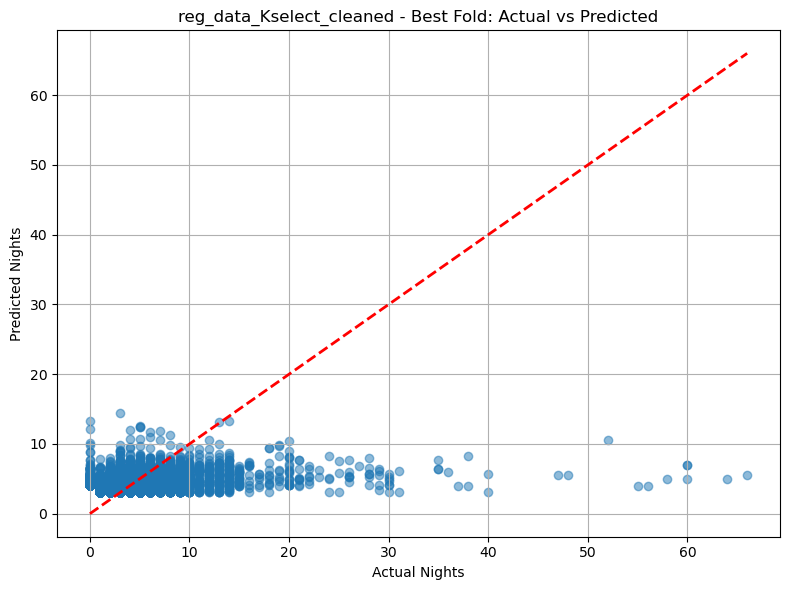
\includegraphics[width=\linewidth]{reg_la_10sc.png}
      \captionof{figure}{Actual Nights vs Predicted Nights}
      \label{fig:2-6}
    }
  }
  \end{figure}

\subsection{Ridge回归模型}
\subsubsection*{原始数据:}
  \begin{figure}[H]
  \centering
  \makebox[\textwidth][c]{%
    % 表格部分
    \parbox{0.48\textwidth}{%
      \centering
      \captionof{table}{Ridge回归模型原始数据训练下五折评估指标}
      \begin{tabular}{lccc}
          \toprule
          折数 & MSE & MAE & R2 \\ \midrule
          Fold 1 & 260.3425 & 7.2925 & 0.3577 \\
          Fold 2 & 5985.8452 & 11.1883 & -17.2513 \\
          Fold 3 & 277.2545 & 6.4498 & 0.2049 \\
          Fold 4 & 274.2829 & 6.3397 & 0.2807 \\
          Fold 5 & 377.1823 & 6.7483 & 0.3639 \\
          Average & 1434.9815 & 7.6037 & -3.2088 \\
          Best & 377.1823 & 6.7483 & 0.3639 \\
          \bottomrule
      \end{tabular}
    }
    \hfill
    % 图像部分
    \parbox{0.48\textwidth}{%
      \centering
      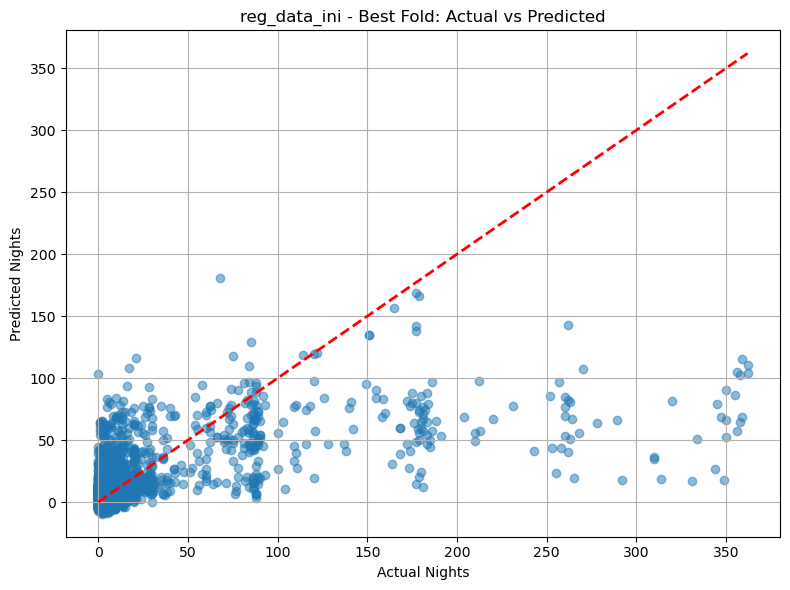
\includegraphics[width=\linewidth]{reg_r_ini.png}
      \captionof{figure}{Actual Nights vs Predicted Nights}
      \label{fig:3-1}
    }
  }
  \end{figure}

\subsubsection*{标准化数据:}
  \begin{figure}[H]
  \centering
  \makebox[\textwidth][c]{%
    % 表格部分
    \parbox{0.48\textwidth}{%
      \centering
      \captionof{table}{Ridge回归模型标准化数据训练下五折评估指标}
      \begin{tabular}{lccc}
          \toprule
          折数 & MSE & MAE & R2 \\ \midrule
          Fold 1 & 262.3633 & 7.4057 & 0.3527 \\
          Fold 2 & 5900.5127 & 11.2737 & -16.9911 \\
          Fold 3 & 277.9904 & 6.4628 & 0.2028 \\
          Fold 4 & 268.0924 & 6.3565 & 0.2970 \\
          Fold 5 & 377.1059 & 6.7486 & 0.3640 \\
          Average & 1417.2129 & 7.6495 & -3.1549 \\
          Best & 377.1059 & 6.7486 & 0.3640 \\
          \bottomrule
      \end{tabular}
    }
    \hfill
    % 图像部分
    \parbox{0.48\textwidth}{%
      \centering
      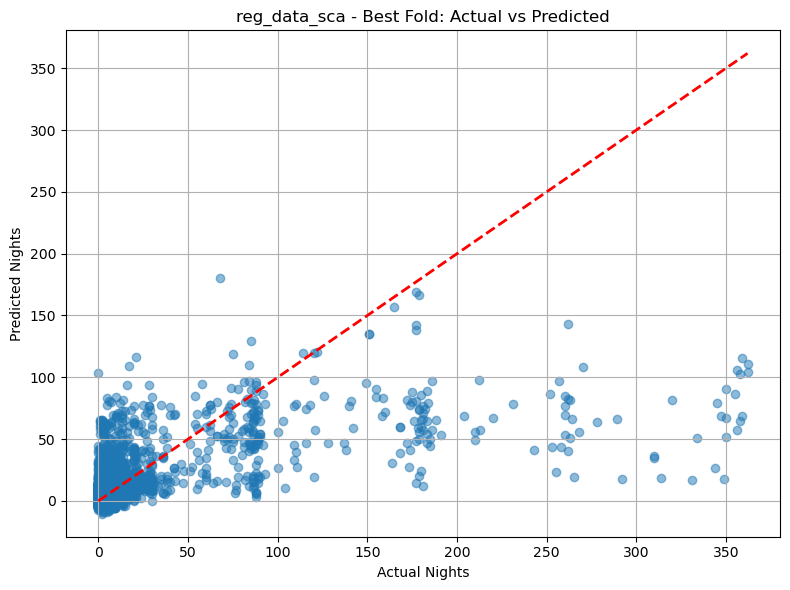
\includegraphics[width=\linewidth]{reg_r_sca.png}
      \captionof{figure}{Actual Nights vs Predicted Nights}
      \label{fig:3-2}
    }
  }
  \end{figure}

\subsubsection*{PCA数据:}
  \begin{figure}[H]
  \centering
  \makebox[\textwidth][c]{%
    % 表格部分
    \parbox{0.48\textwidth}{%
      \centering
      \captionof{table}{Ridge回归模型PCA数据训练下五折评估指标}
      \begin{tabular}{lccc}
          \toprule
          折数 & MSE & MAE & R2 \\ \midrule
          Fold 1 & 312.1705 & 7.1230 & 0.2298 \\
          Fold 2 & 3546.0854 & 11.3339 & -9.8123 \\
          Fold 3 & 307.5685 & 6.1770 & 0.1180 \\
          Fold 4 & 341.9265 & 6.1010 & 0.1033 \\
          Fold 5 & 524.3387 & 7.0609 & 0.1157 \\
          Average & 1006.4179 & 7.5592 & -1.8491 \\
          Best & 312.1705 & 7.1230 & 0.2298 \\
          \bottomrule
      \end{tabular}
    }
    \hfill
    % 图像部分
    \parbox{0.48\textwidth}{%
      \centering
      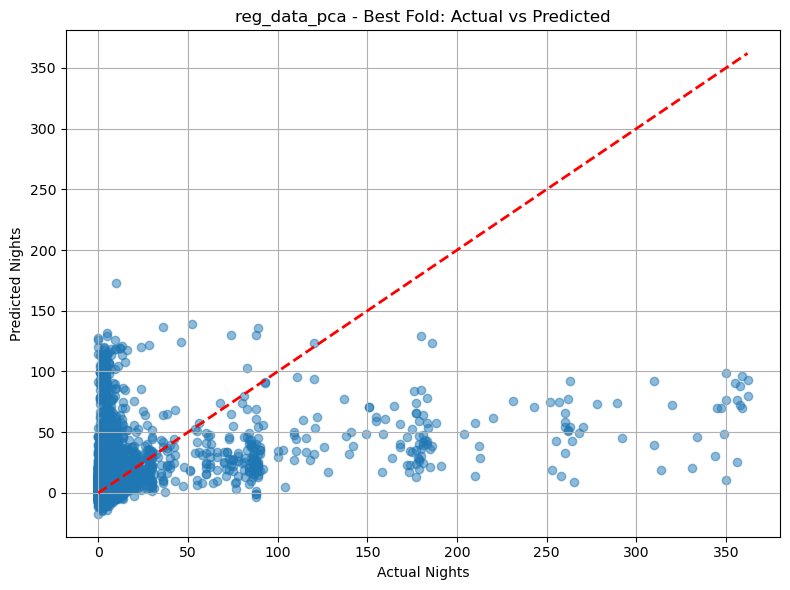
\includegraphics[width=\linewidth]{reg_r_pca.png}
      \captionof{figure}{Actual Nights vs Predicted Nights}
      \label{fig:3-3}
    }
  }
  \end{figure}

\subsubsection*{10项特征提取数据:}
  \begin{figure}[H]
  \centering
  \makebox[\textwidth][c]{%
    % 表格部分
    \parbox{0.48\textwidth}{%
      \centering
      \captionof{table}{Ridge回归模型10项特征提取数据训练下五折评估指标}
      \begin{tabular}{lccc}
          \toprule
          折数 & MSE & MAE & R2 \\ \midrule
          Fold 1 & 278.6263 & 6.3046 & 0.3125 \\
          Fold 2 & 2031.7844 & 8.2071 & -5.1951 \\
          Fold 3 & 288.3358 & 5.9861 & 0.1731 \\
          Fold 4 & 272.6580 & 5.7056 & 0.2850 \\
          Fold 5 & 394.9882 & 6.3756 & 0.3338 \\
          Average & 653.2786 & 6.5158 & -0.8181 \\
          Best & 394.9882 & 6.3756 & 0.3338 \\
          \bottomrule
      \end{tabular}
    }
    \hfill
    % 图像部分
    \parbox{0.48\textwidth}{%
      \centering
      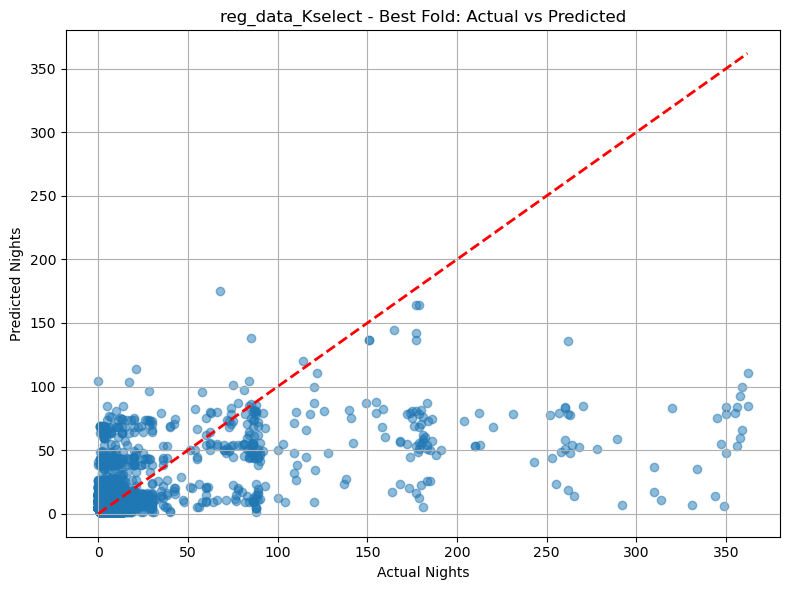
\includegraphics[width=\linewidth]{reg_r_10s.png}
      \captionof{figure}{Actual Nights vs Predicted Nights}
      \label{fig:3-4}
    }
  }
  \end{figure}

\subsubsection*{50项特征提取数据:}
  \begin{figure}[H]
  \centering
  \makebox[\textwidth][c]{%
    % 表格部分
    \parbox{0.48\textwidth}{%
      \centering
      \captionof{table}{Ridge回归模型50项特征提取数据训练下五折评估指标}
      \begin{tabular}{lccc}
          \toprule
          折数 & MSE & MAE & R2 \\ \midrule
          Fold 1 & 255.2087 & 6.6430 & 0.3703 \\
          Fold 2 & 4620.5263 & 9.6299 & -13.0883 \\
          Fold 3 & 278.7732 & 5.9341 & 0.2005 \\
          Fold 4 & 269.4585 & 6.0046 & 0.2934 \\
          Fold 5 & 382.4843 & 6.5596 & 0.3549 \\
          Average & 1161.2902 & 6.9542 & -2.3738 \\
          Best & 255.2087 & 6.6430 & 0.3703 \\
          \bottomrule
      \end{tabular}
    }
    \hfill
    % 图像部分
    \parbox{0.48\textwidth}{%
      \centering
      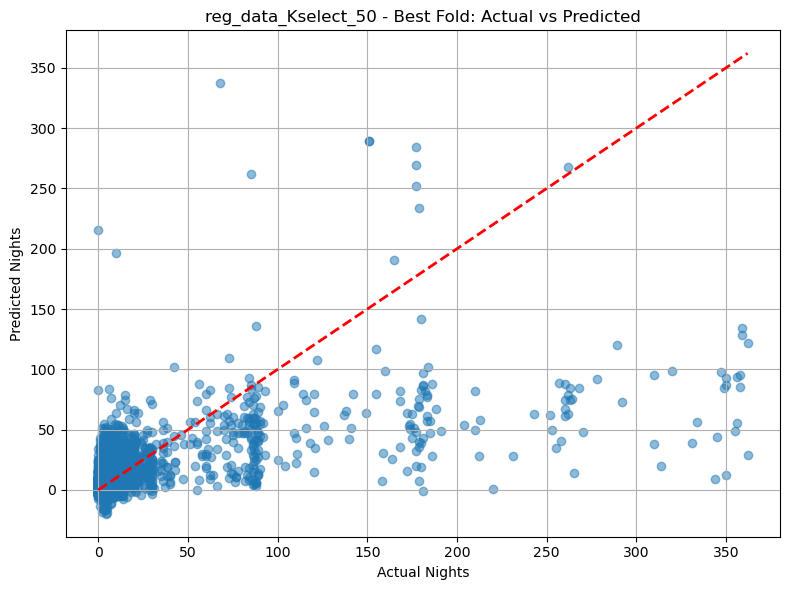
\includegraphics[width=\linewidth]{reg_r_50s.png}
      \captionof{figure}{Actual Nights vs Predicted Nights}
      \label{fig:3-5}
    }
  }
  \end{figure}

\subsubsection*{清洗后的10项特征提取数据:}
  \begin{figure}[H]
  \centering
  \makebox[\textwidth][c]{%
    % 表格部分
    \parbox{0.48\textwidth}{%
      \centering
      \captionof{table}{Ridge回归模型清洗后的10项特征提取数据训练下五折评估指标}
      \begin{tabular}{lccc}
          \toprule
          折数 & MSE & MAE & R2 \\ \midrule
          Fold 1 & 18.3104 & 2.2219 & 0.0742 \\
          Fold 2 & 22.1839 & 2.4768 & 0.0034 \\
          Fold 3 & 18.6018 & 2.3348 & 0.0930 \\
          Fold 4 & 17.2910 & 2.1480 & 0.0834 \\
          Fold 5 & 13.5112 & 2.1709 & 0.0798 \\
          Average & 17.9797 & 2.2705 & 0.0668 \\
          Best & 18.6018 & 2.3348 & 0.0930 \\
          \bottomrule
      \end{tabular}
    }
    \hfill
    % 图像部分
    \parbox{0.48\textwidth}{%
      \centering
      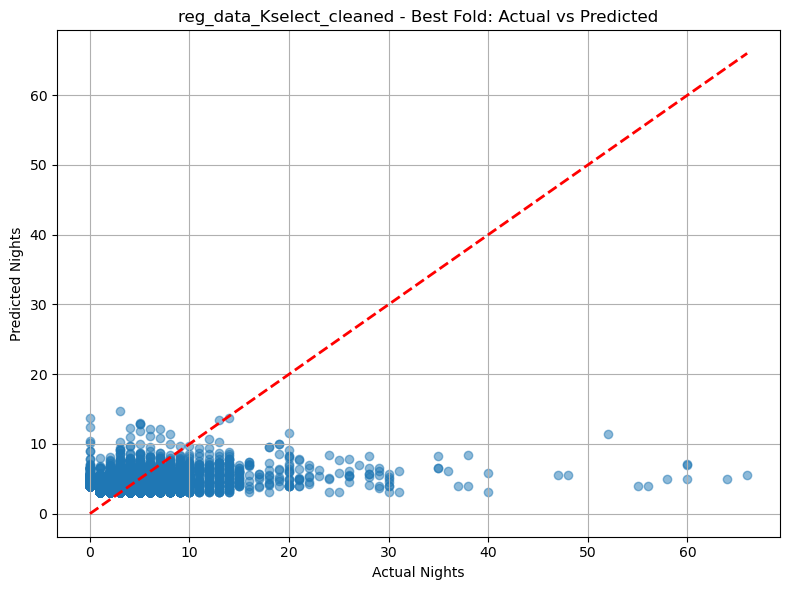
\includegraphics[width=\linewidth]{reg_r_10sc.png}
      \captionof{figure}{Actual Nights vs Predicted Nights}
      \label{fig:3-6}
    }
  }
  \end{figure}

\subsection{随机森林模型}
\subsubsection*{标准化数据:}
  \begin{figure}[H]
  \centering
  \makebox[\textwidth][c]{%
    % 表格部分
    \parbox{0.48\textwidth}{%
      \centering
      \captionof{table}{随机森林模型标准化数据训练下五折评估指标}
      \begin{tabular}{lccc}
          \toprule
          折数 & MSE & MAE & R2 \\ \midrule
          Fold 1 & 211.4701 & 4.2081 & 0.4782 \\
          Fold 2 & 304.0424 & 5.5388 & 0.0730 \\
          Fold 3 & 184.8663 & 3.8326 & 0.4698 \\
          Fold 4 & 183.9467 & 3.6730 & 0.5176 \\
          Fold 5 & 211.6675 & 3.8089 & 0.6430 \\
          Average & 219.1986 & 4.2123 & 0.4363 \\
          Best & 211.6675 & 3.8089 & 0.6430 \\
          \bottomrule
      \end{tabular}
    }
    \hfill
    % 图像部分
    \parbox{0.48\textwidth}{%
      \centering
      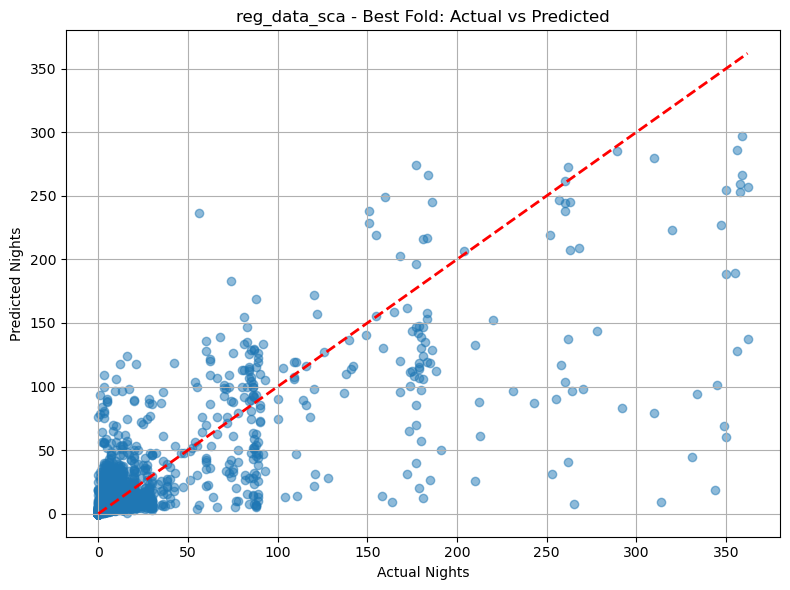
\includegraphics[width=\linewidth]{reg_rf_sca.png}
      \captionof{figure}{Actual Nights vs Predicted Nights}
      \label{fig:4-1}
    }
  }
  \end{figure}

\subsubsection*{PCA数据:}
  \begin{figure}[H]
  \centering
  \makebox[\textwidth][c]{%
    % 表格部分
    \parbox{0.48\textwidth}{%
      \centering
      \captionof{table}{随机森林模型PCA数据训练下五折评估指标}
      \begin{tabular}{lccc}
          \toprule
          折数 & MSE & MAE & R2 \\ \midrule
          Fold 1 & 284.2872 & 5.3487 & 0.2986 \\
          Fold 2 & 383.5303 & 6.5348 & -0.1694 \\
          Fold 3 & 257.9379 & 4.7256 & 0.2603 \\
          Fold 4 & 264.6351 & 4.8651 & 0.3060 \\
          Fold 5 & 353.9304 & 5.4302 & 0.4031 \\
          Average & 308.8642 & 5.3809 & 0.2197 \\
          Best & 353.9304 & 5.4302 & 0.4031 \\
          \bottomrule
      \end{tabular}
    }
    \hfill
    % 图像部分
    \parbox{0.48\textwidth}{%
      \centering
      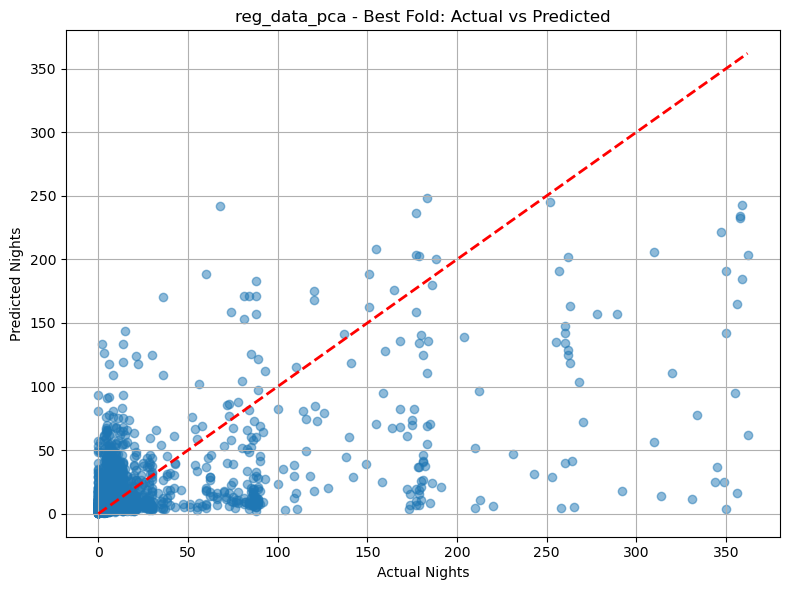
\includegraphics[width=\linewidth]{reg_rf_pca.png}
      \captionof{figure}{Actual Nights vs Predicted Nights}
      \label{fig:4-2}
    }
  }
  \end{figure}

\subsubsection*{10项特征提取数据:}
  \begin{figure}[H]
  \centering
  \makebox[\textwidth][c]{%
    % 表格部分
    \parbox{0.48\textwidth}{%
      \centering
      \captionof{table}{随机森林模型10项特征提取数据训练下五折评估指标}
      \begin{tabular}{lccc}
          \toprule
          折数 & MSE & MAE & R2 \\ \midrule
          Fold 1 & 196.5421 & 4.1510 & 0.5151 \\
          Fold 2 & 244.8156 & 4.8132 & 0.2535 \\
          Fold 3 & 232.4115 & 4.2022 & 0.3335 \\
          Fold 4 & 203.0266 & 3.8641 & 0.4676 \\
          Fold 5 & 255.8492 & 4.3461 & 0.5685 \\
          Average & 226.5290 & 4.2753 & 0.4276 \\
          Best & 255.8492 & 4.3461 & 0.5685 \\
          \bottomrule
      \end{tabular}
    }
    \hfill
    % 图像部分
    \parbox{0.48\textwidth}{%
      \centering
      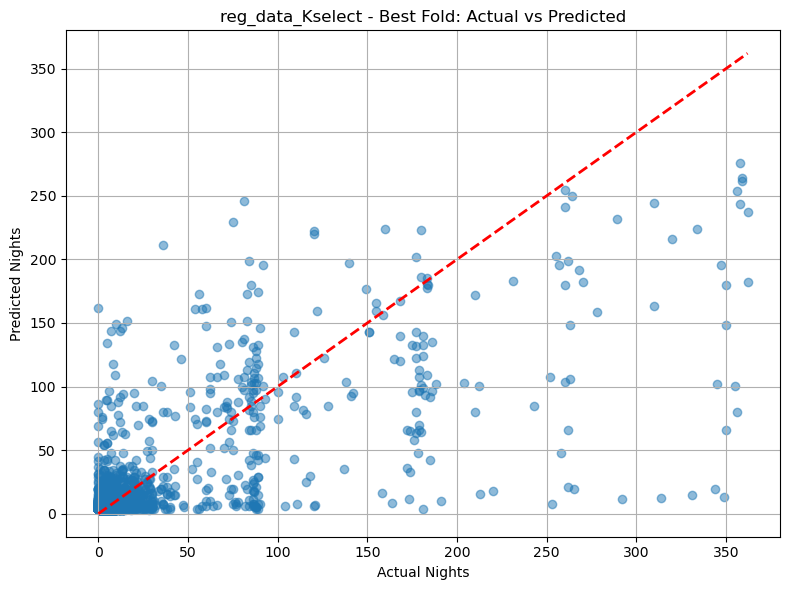
\includegraphics[width=\linewidth]{reg_rf_10s.png}
      \captionof{figure}{Actual Nights vs Predicted Nights}
      \label{fig:4-3}
    }
  }
  \end{figure}

\subsubsection*{50项特征提取数据:}
  \begin{figure}[H]
  \centering
  \makebox[\textwidth][c]{%
    % 表格部分
    \parbox{0.48\textwidth}{%
      \centering
      \captionof{table}{随机森林模型50项特征提取数据训练下五折评估指标}
      \begin{tabular}{lccc}
          \toprule
          折数 & MSE & MAE & R2 \\ \midrule
          Fold 1 & 197.2213 & 4.2446 & 0.5134 \\
          Fold 2 & 296.4568 & 5.3218 & 0.0961 \\
          Fold 3 & 193.1003 & 3.7999 & 0.4462 \\
          Fold 4 & 183.1465 & 3.6573 & 0.5197 \\
          Fold 5 & 234.9864 & 4.1050 & 0.6037 \\
          Average & 220.9823 & 4.2257 & 0.4358 \\
          Best & 234.9864 & 4.1050 & 0.6037 \\
          \bottomrule
      \end{tabular}
    }
    \hfill
    % 图像部分
    \parbox{0.48\textwidth}{%
      \centering
      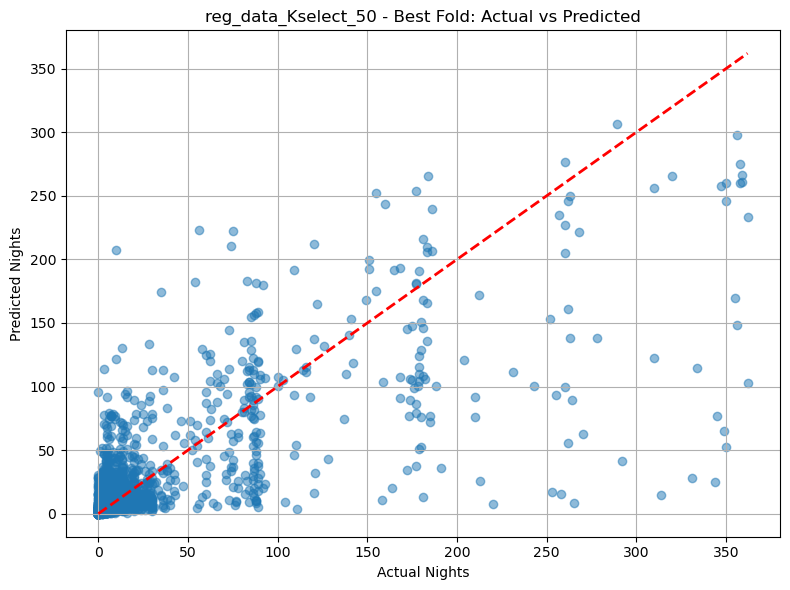
\includegraphics[width=\linewidth]{reg_rf_50s.png}
      \captionof{figure}{Actual Nights vs Predicted Nights}
      \label{fig:4-4}
    }
  }
  \end{figure}

\subsubsection*{清洗后的10项特征提取数据:}
  \begin{figure}[H]
  \centering
  \makebox[\textwidth][c]{%
    % 表格部分
    \parbox{0.48\textwidth}{%
      \centering
      \captionof{table}{随机森林模型清洗后的10项特征提取数据训练下五折评估指标}
      \begin{tabular}{lccc}
          \toprule
          折数 & MSE & MAE & R2 \\ \midrule
          Fold 1 & 17.7608 & 2.1529 & 0.1020 \\
          Fold 2 & 21.3350 & 2.4645 & 0.0415 \\
          Fold 3 & 17.6212 & 2.2466 & 0.1408 \\
          Fold 4 & 16.5217 & 2.0615 & 0.1242 \\
          Fold 5 & 12.9729 & 2.0930 & 0.1165 \\
          Average & 17.2423 & 2.2037 & 0.1050 \\
          Best & 17.6212 & 2.2466 & 0.1408 \\
          \bottomrule
      \end{tabular}
    }
    \hfill
    % 图像部分
    \parbox{0.48\textwidth}{%
      \centering
      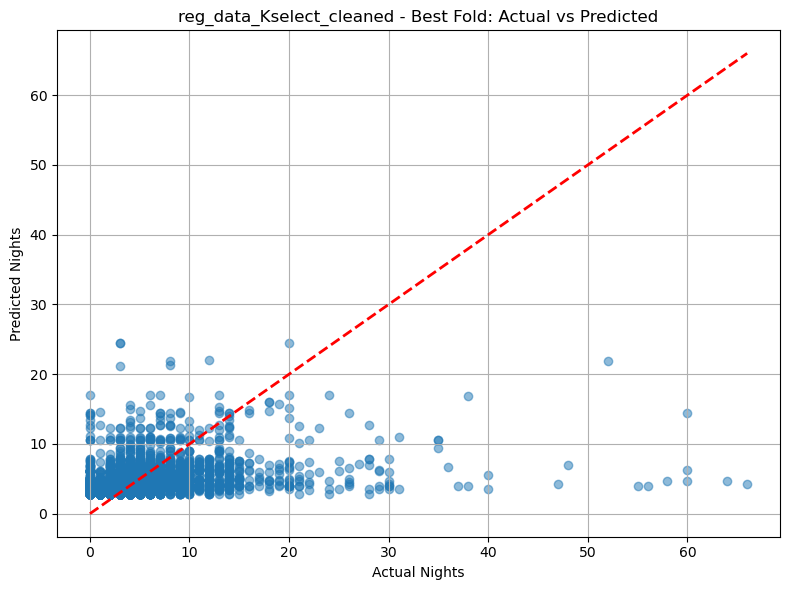
\includegraphics[width=\linewidth]{reg_rf_10sc.png}
      \captionof{figure}{Actual Nights vs Predicted Nights}
      \label{fig:4-5}
    }
  }
  \end{figure}

\subsection{SVR}
\subsubsection*{PCA数据:}
  \begin{figure}[H]
  \centering
  \makebox[\textwidth][c]{%
    % 表格部分
    \parbox{0.48\textwidth}{%
      \centering
      \captionof{table}{SVR在PCA数据训练下五折评估指标}
      \begin{tabular}{lccc}
          \toprule
          折数 & MSE & MAE & R2 \\ \midrule
          Fold 1 & 364.5163 & 4.2061 & 0.1006 \\
          Fold 2 & 280.4139 & 3.8682 & 0.1450 \\
          Fold 3 & 303.5393 & 3.8196 & 0.1295 \\
          Fold 4 & 317.7262 & 3.7525 & 0.1668 \\
          Fold 5 & 476.1165 & 4.6908 & 0.1970 \\
          Average & 348.4624 & 4.0674 & 0.1478 \\
          Best & 476.1165 & 4.6908 & 0.1970 \\
          \bottomrule
      \end{tabular}
    }
    \hfill
    % 图像部分
    \parbox{0.48\textwidth}{%
      \centering
      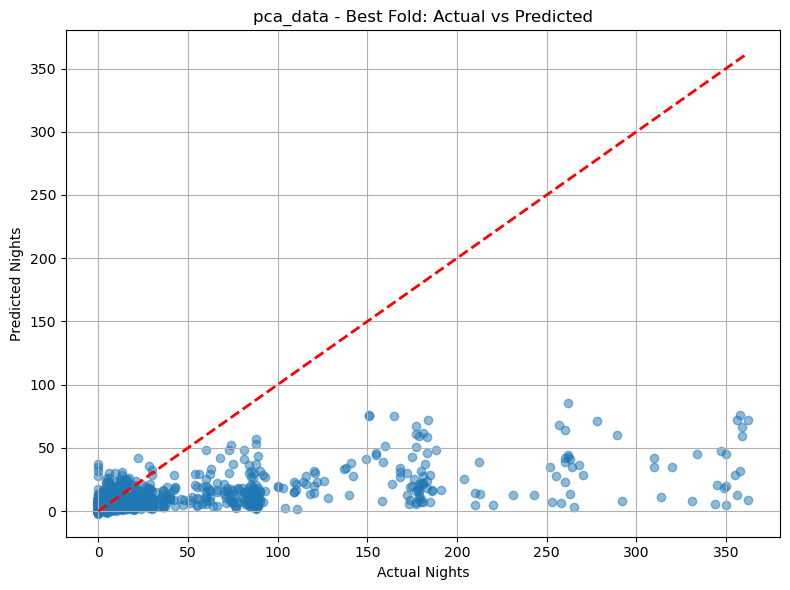
\includegraphics[width=\linewidth]{reg_svr_pca.png}
      \captionof{figure}{Actual Nights vs Predicted Nights}
      \label{fig:5-1}
    }
  }
  \end{figure}

\subsubsection*{10项特征提取数据:}
  \begin{figure}[H]
  \centering
  \makebox[\textwidth][c]{%
    % 表格部分
    \parbox{0.48\textwidth}{%
      \centering
      \captionof{table}{SVR在10项特征提取数据训练下五折评估指标}
      \begin{tabular}{lccc}
          \toprule
          折数 & MSE & MAE & R2 \\ \midrule
          Fold 1 & 290.6699 & 4.0755 & 0.2828 \\
          Fold 2 & 258.7043 & 4.1154 & 0.2112 \\
          Fold 3 & 274.7173 & 3.9747 & 0.2122 \\
          Fold 4 & 290.2829 & 3.7802 & 0.2388 \\
          Fold 5 & 379.6527 & 4.4638 & 0.3597 \\
          Average & 298.8054 & 4.0819 & 0.2609 \\
          Best & 379.6527 & 4.4638 & 0.3597 \\
          \bottomrule
      \end{tabular}
    }
    \hfill
    % 图像部分
    \parbox{0.48\textwidth}{%
      \centering
      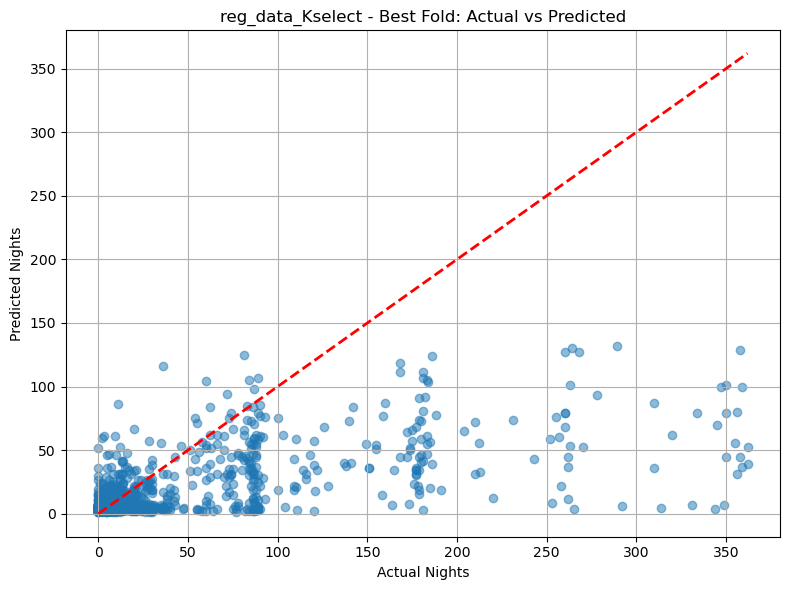
\includegraphics[width=\linewidth]{reg_svr_10s.png}
      \captionof{figure}{Actual Nights vs Predicted Nights}
      \label{fig:5-2}
    }
  }
  \end{figure}

\subsubsection*{50项特征提取数据:}
  \begin{figure}[H]
  \centering
  \makebox[\textwidth][c]{%
    % 表格部分
    \parbox{0.48\textwidth}{%
      \centering
      \captionof{table}{SVR在50项特征提取数据训练下五折评估指标}
      \begin{tabular}{lccc}
          \toprule
          折数 & MSE & MAE & R2 \\ \midrule
          Fold 1 & 355.2848 & 4.0209 & 0.1234 \\
          Fold 2 & 275.6529 & 3.9686 & 0.1595 \\
          Fold 3 & 300.5682 & 3.8578 & 0.1380 \\
          Fold 4 & 327.3428 & 3.7428 & 0.1416 \\
          Fold 5 & 468.6323 & 4.5820 & 0.2096 \\
          Average & 345.4962 & 4.0344 & 0.1544 \\
          Best & 468.6323 & 4.5820 & 0.2096 \\
          \bottomrule
      \end{tabular}
    }
    \hfill
    % 图像部分
    \parbox{0.48\textwidth}{%
      \centering
      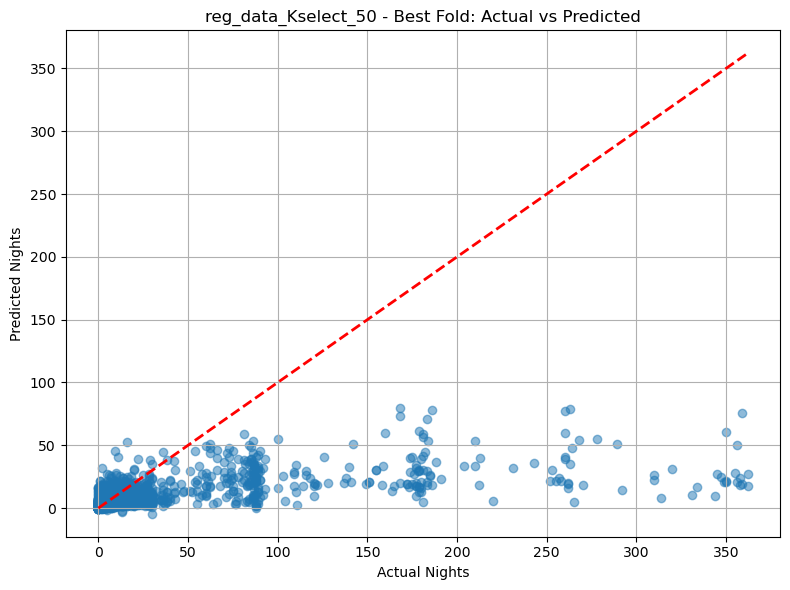
\includegraphics[width=\linewidth]{reg_svr_50s.png}
      \captionof{figure}{Actual Nights vs Predicted Nights}
      \label{fig:5-3}
    }
  }
  \end{figure}

\subsubsection*{清洗后的10项特征提取数据:}
  \begin{figure}[H]
  \centering
  \makebox[\textwidth][c]{%
    % 表格部分
    \parbox{0.48\textwidth}{%
      \centering
      \captionof{table}{SVR清洗后的10项特征提取数据训练下五折评估指标}
      \begin{tabular}{lccc}
          \toprule
          折数 & MSE & MAE & R2 \\ \midrule
          Fold 1 & 18.7741 & 2.1039 & 0.0508 \\
          Fold 2 & 22.6115 & 2.3760 & -0.0158 \\
          Fold 3 & 19.0037 & 2.1750 & 0.0734 \\
          Fold 4 & 17.6689 & 2.0315 & 0.0633 \\
          Fold 5 & 13.7260 & 2.0511 & 0.0652 \\
          Average & 18.3568 & 2.1475 & 0.0474 \\
          Best & 19.0037 & 2.1750 & 0.0734 \\
          \bottomrule
      \end{tabular}
    }
    \hfill
    % 图像部分
    \parbox{0.48\textwidth}{%
      \centering
      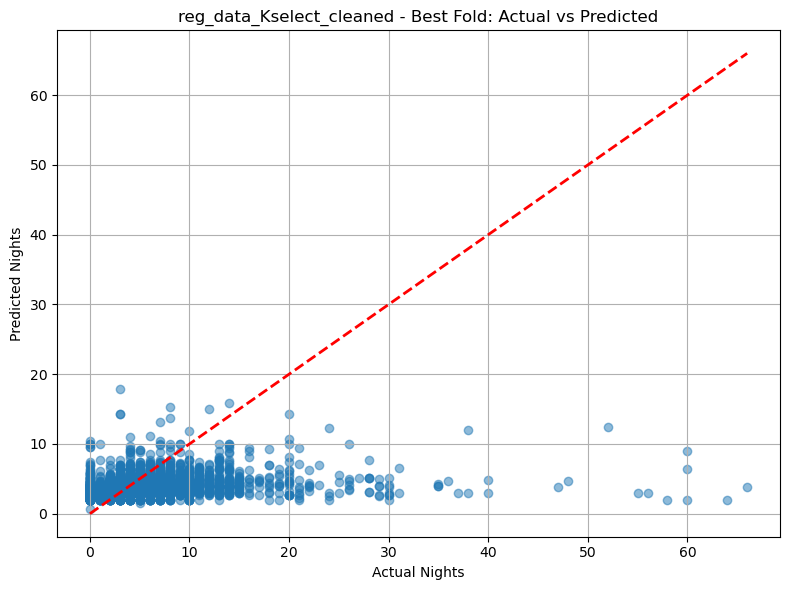
\includegraphics[width=\linewidth]{reg_svr_10sc.png}
      \captionof{figure}{Actual Nights vs Predicted Nights}
      \label{fig:5-4}
    }
  }
  \end{figure}
\renewcommand{\thesection}{A\arabic{section}}

\section{分类任务结果}
由于数据图表实在太多,故仅仅在此展现平均之后的数据,就不再展示每一折的评估指标的结果。
\subsection{KNN}
\subsubsection*{原始数据}
\begin{table}[H]
  \centering
  \caption{KNN在原始数据训练下各项评估指标均值}
  \begin{tabular}{llll}
  \toprule
  Accuracy & Precision\_macro & Recall\_macro & F1\_macro \\
  0.6989 & 0.4520 & 0.3482 & 0.3647 \\
  \midrule
  AUC & Precision\_weighted & Recall\_weighted & F1\_weighted \\
  0.6707 & 0.6527 & 0.6989 & 0.6646 \\
  \bottomrule
  \end{tabular}
\end{table}

\begin{figure}[H]
\centering
\begin{minipage}[t]{0.45\textwidth}
  \centering
  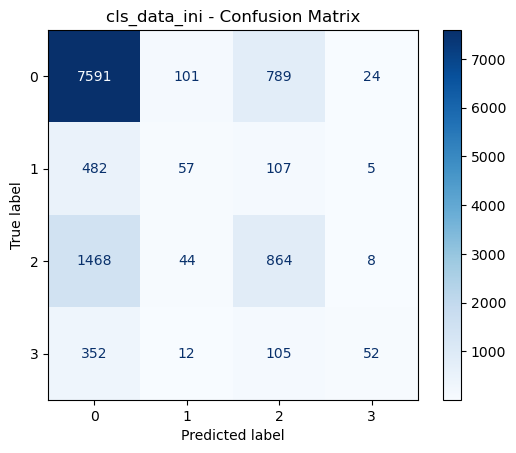
\includegraphics[width=\linewidth]{cls_knn_ini1.png}
  \caption{混淆矩阵}
  \label{fig:20}
\end{minipage}
\hfill
\begin{minipage}[t]{0.52\textwidth}
  \centering
  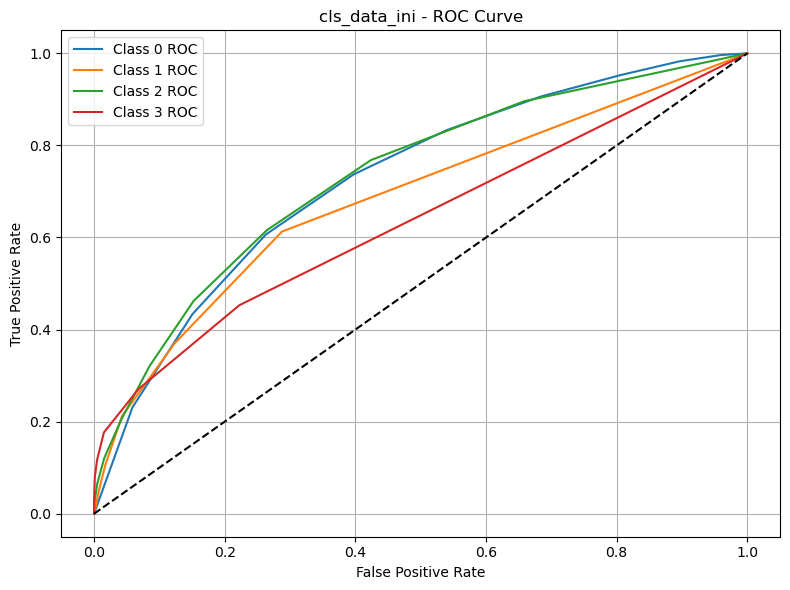
\includegraphics[width=\linewidth]{cls_knn_ini2.png}
  \caption{ROC曲线}
  \label{fig:21}
\end{minipage}
\end{figure}


\subsubsection*{标准化数据}
\begin{table}[H]
  \centering
  \caption{KNN在标准化数据训练下各项评估指标均值}
  \begin{tabular}{llll}
  \toprule
  Accuracy & Precision\_macro & Recall\_macro & F1\_macro \\
  0.8290 & 0.6873 & 0.5133 & 0.5292 \\
  \midrule
  AUC & Precision\_weighted & Recall\_weighted & F1\_weighted \\
  0.8297 & 0.8149 & 0.8290 & 0.8086 \\
  \bottomrule
  \end{tabular}
\end{table}

\begin{figure}[H]
\centering
\begin{minipage}[t]{0.45\textwidth}
  \centering
  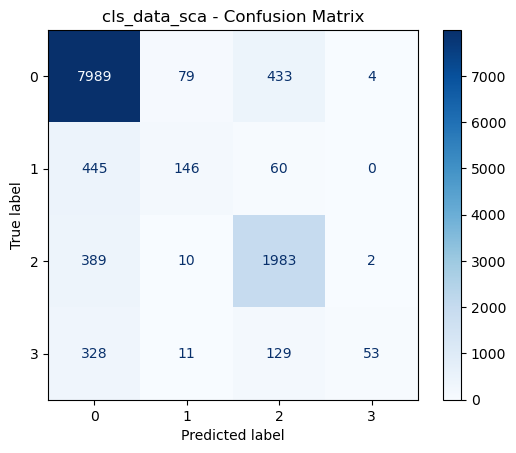
\includegraphics[width=\linewidth]{cls_knn_sca1.png}
  \caption{混淆矩阵}
  \label{fig:22}
\end{minipage}
\hfill
\begin{minipage}[t]{0.52\textwidth}
  \centering
  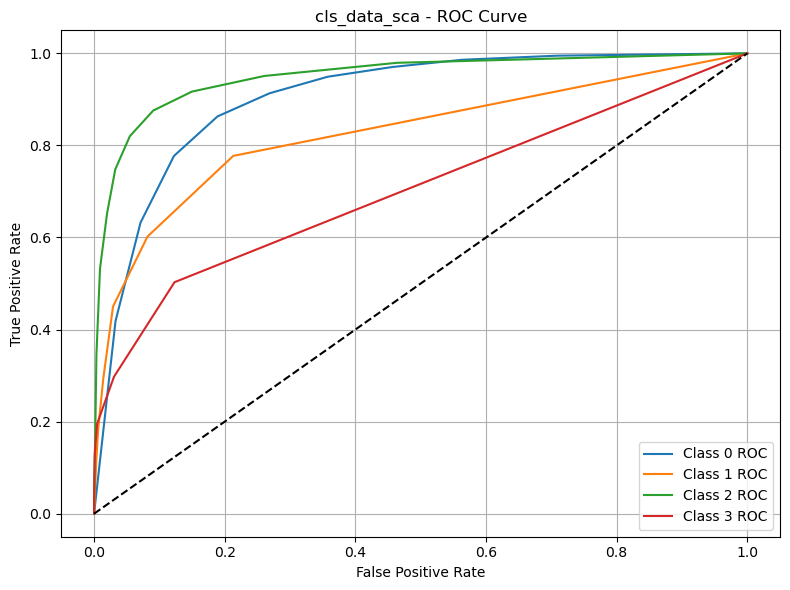
\includegraphics[width=\linewidth]{cls_knn_sca2.png}
  \caption{ROC曲线}
  \label{fig:23}
\end{minipage}
\end{figure}

\subsubsection*{LDA降维数据}
\begin{table}[H]
  \centering
  \caption{KNN在LDA降维数据训练下各项评估指标均值}
  \begin{tabular}{llll}
  \toprule
  Accuracy & Precision\_macro & Recall\_macro & F1\_macro \\
  0.8748 & 0.7251 & 0.6478 & 0.6750 \\
  \midrule
  AUC & Precision\_weighted & Recall\_weighted & F1\_weighted \\
  0.8954 & 0.8659 & 0.8748 & 0.8683 \\
  \bottomrule
  \end{tabular}
\end{table}

\begin{figure}[H]
\centering
\begin{minipage}[t]{0.45\textwidth}
  \centering
  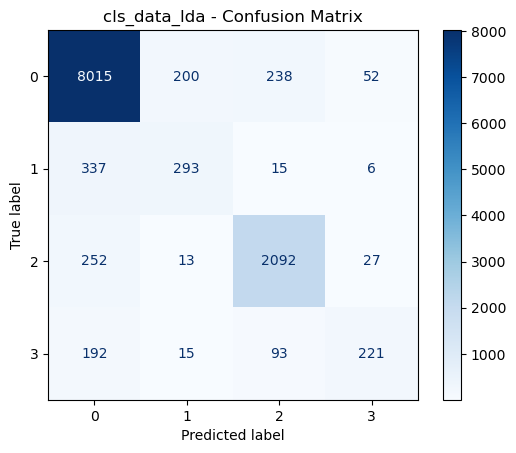
\includegraphics[width=\linewidth]{cls_knn_lda1.png}
  \caption{混淆矩阵}
  \label{fig:24}
\end{minipage}
\hfill
\begin{minipage}[t]{0.52\textwidth}
  \centering
  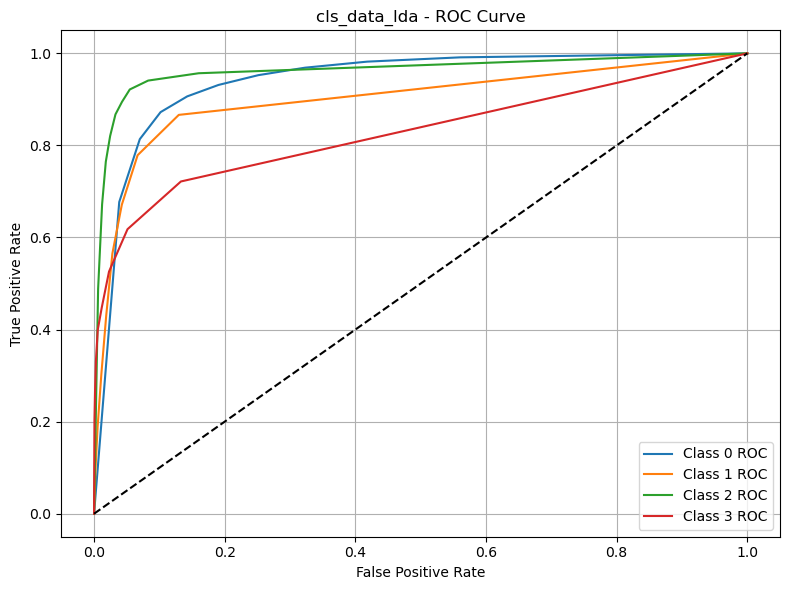
\includegraphics[width=\linewidth]{cls_knn_lda2.png}
  \caption{ROC曲线}
  \label{fig:25}
\end{minipage}
\end{figure}

\subsubsection*{10项特征提取数据}
\begin{table}[H]
  \centering
  \caption{KNN在10项特征提取数据训练下各项评估指标均值}
  \begin{tabular}{llll}
  \toprule
  Accuracy & Precision\_macro & Recall\_macro & F1\_macro \\
  0.8116 & 0.6130 & 0.6181 & 0.6073 \\
  \midrule
  AUC & Precision\_weighted & Recall\_weighted & F1\_weighted \\
  0.8466 & 0.8196 & 0.8116 & 0.8137 \\
  \bottomrule
  \end{tabular}
\end{table}

\begin{figure}[H]
\centering
\begin{minipage}[t]{0.45\textwidth}
  \centering
  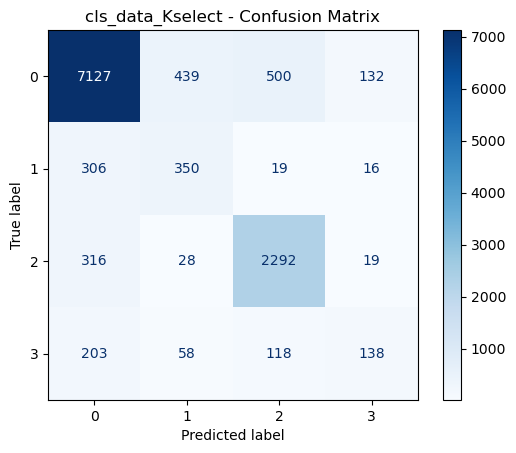
\includegraphics[width=\linewidth]{cls_knn_10s.png}
  \caption{混淆矩阵}
  \label{fig:26}
\end{minipage}
\hfill
\begin{minipage}[t]{0.52\textwidth}
  \centering
  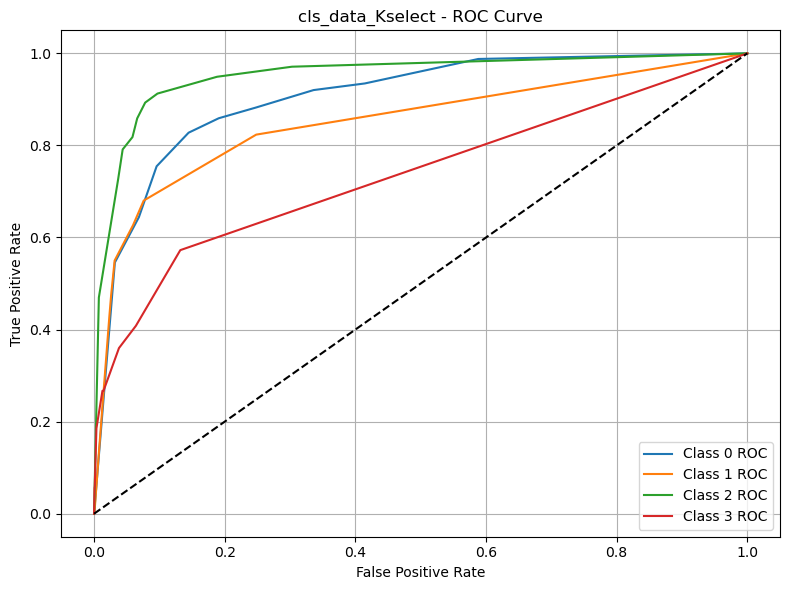
\includegraphics[width=\linewidth]{cls_knn_10s2.png}
  \caption{ROC曲线}
  \label{fig:27}
\end{minipage}
\end{figure}

\subsubsection*{50项特征提取数据}
\begin{table}[H]
  \centering
  \caption{KNN在50项特征提取数据训练下各项评估指标均值}
  \begin{tabular}{llll}
  \toprule
  Accuracy & Precision\_macro & Recall\_macro & F1\_macro \\
  0.8740 & 0.7401 & 0.6211 & 0.6580 \\
  \midrule
  AUC & Precision\_weighted & Recall\_weighted & F1\_weighted \\
  0.8779 & 0.8624 & 0.8740 & 0.8640 \\
  \bottomrule
  \end{tabular}
\end{table}

\begin{figure}[H]
\centering
\begin{minipage}[t]{0.45\textwidth}
  \centering
  \includegraphics[width=\linewidth]{cls_knn_50s.png}
  \caption{混淆矩阵}
  \label{fig:28}
\end{minipage}
\hfill
\begin{minipage}[t]{0.52\textwidth}
  \centering
  \includegraphics[width=\linewidth]{cls_knn_50s2.png}
  \caption{ROC曲线}
  \label{fig:29}
\end{minipage}
\end{figure}


\subsubsection*{清洗后的10项特征提取数据}
\begin{table}[H]
  \centering
  \caption{KNN在清洗后的10项特征提取数据训练下各项评估指标均值}
  \begin{tabular}{llll}
  \toprule
  Accuracy & Precision\_macro & Recall\_macro & F1\_macro \\
  0.8482 & 0.4754 & 0.4938 & 0.4721 \\
  \midrule
  AUC & Precision\_weighted & Recall\_weighted & F1\_weighted \\
  0.8005 & 0.8500 & 0.8482 & 0.8478 \\
  \bottomrule
  \end{tabular}
\end{table}

\begin{figure}[H]
\centering
\begin{minipage}[t]{0.45\textwidth}
  \centering
  \includegraphics[width=\linewidth]{cls_knn_10sc.png}
  \caption{混淆矩阵}
  \label{fig:30}
\end{minipage}
\hfill
\begin{minipage}[t]{0.52\textwidth}
  \centering
  \includegraphics[width=\linewidth]{cls_knn_10sc2.png}
  \caption{ROC曲线}
  \label{fig:31}
\end{minipage}
\end{figure}


\subsection{Logistic}
\subsubsection*{原始数据}
\begin{table}[H]
  \centering
  \caption{Logistic在原始数据训练下各项评估指标均值}
  \begin{tabular}{llll}
  \toprule
  Accuracy & Precision\_macro & Recall\_macro & F1\_macro \\
  0.8803 & 0.7750 & 0.6353 & 0.6764 \\
  \midrule
  AUC & Precision\_weighted & Recall\_weighted & F1\_weighted \\
  0.9332 & 0.8716 & 0.8803 & 0.8706 \\
  \bottomrule
  \end{tabular}
\end{table}

\begin{figure}[H]
\centering
\begin{minipage}[t]{0.45\textwidth}
  \centering
  \includegraphics[width=\linewidth]{cls_log_ini1.png}
  \caption{混淆矩阵}
  \label{fig:32}
\end{minipage}
\hfill
\begin{minipage}[t]{0.52\textwidth}
  \centering
  \includegraphics[width=\linewidth]{cls_log_ini2.png}
  \caption{ROC曲线}
  \label{fig:13}
\end{minipage}
\end{figure}


\subsubsection*{标准化数据}
\begin{table}[H]
  \centering
  \caption{Logistic在标准化数据训练下各项评估指标均值}
  \begin{tabular}{llll}
  \toprule
  Accuracy & Precision\_macro & Recall\_macro & F1\_macro \\
  0.8790 & 0.7716 & 0.6322 & 0.6725 \\
  \midrule
  AUC & Precision\_weighted & Recall\_weighted & F1\_weighted \\
  0.9323 & 0.8704 & 0.8790 & 0.8691 \\
  \bottomrule
  \end{tabular}
\end{table}

\begin{figure}[H]
\centering
\begin{minipage}[t]{0.45\textwidth}
  \centering
  \includegraphics[width=\linewidth]{cls_log_sca1.png}
  \caption{混淆矩阵}
  \label{fig:33}
\end{minipage}
\hfill
\begin{minipage}[t]{0.52\textwidth}
  \centering
  \includegraphics[width=\linewidth]{cls_log_sca2.png}
  \caption{ROC曲线}
  \label{fig:34}
\end{minipage}
\end{figure}

\subsubsection*{LDA降维数据}
\begin{table}[H]
  \centering
  \caption{Logistic在LDA降维数据训练下各项评估指标均值}
  \begin{tabular}{llll}
  \toprule
  Accuracy & Precision\_macro & Recall\_macro & F1\_macro \\
  0.8809 & 0.7675 & 0.6418 & 0.6801 \\
  \midrule
  AUC & Precision\_weighted & Recall\_weighted & F1\_weighted \\
  0.9426 & 0.8721 & 0.8809 & 0.8721 \\
  \bottomrule
  \end{tabular}
\end{table}

\begin{figure}[H]
\centering
\begin{minipage}[t]{0.45\textwidth}
  \centering
  \includegraphics[width=\linewidth]{cls_log_lda1.png}
  \caption{混淆矩阵}
  \label{fig:35}
\end{minipage}
\hfill
\begin{minipage}[t]{0.52\textwidth}
  \centering
  \includegraphics[width=\linewidth]{cls_log_lda2.png}
  \caption{ROC曲线}
  \label{fig:36}
\end{minipage}
\end{figure}

\subsubsection*{10项特征提取数据}
\begin{table}[H]
  \centering
  \caption{Logistic在10项特征提取数据训练下各项评估指标均值}
  \begin{tabular}{llll}
  \toprule
  Accuracy & Precision\_macro & Recall\_macro & F1\_macro \\
  0.8486 & 0.7309 & 0.5551 & 0.6013 \\
  \midrule
  AUC & Precision\_weighted & Recall\_weighted & F1\_weighted \\
  0.9018 & 0.8370 & 0.8486 & 0.8327 \\
  \bottomrule
  \end{tabular}
\end{table}

\begin{figure}[H]
\centering
\begin{minipage}[t]{0.45\textwidth}
  \centering
  \includegraphics[width=\linewidth]{cls_log_10s.png}
  \caption{混淆矩阵}
  \label{fig:37}
\end{minipage}
\hfill
\begin{minipage}[t]{0.52\textwidth}
  \centering
  \includegraphics[width=\linewidth]{cls_log_10s2.png}
  \caption{ROC曲线}
  \label{fig:38}
\end{minipage}
\end{figure}

\subsubsection*{50项特征提取数据}
\begin{table}[H]
  \centering
  \caption{Logistic在50项特征提取数据训练下各项评估指标均值}
  \begin{tabular}{llll}
  \toprule
  Accuracy & Precision\_macro & Recall\_macro & F1\_macro \\
  0.8812 & 0.7658 & 0.6315 & 0.6700 \\
  \midrule
  AUC & Precision\_weighted & Recall\_weighted & F1\_weighted \\
  0.9269 & 0.8715 & 0.8812 & 0.8713 \\
  \bottomrule
  \end{tabular}
\end{table}

\begin{figure}[H]
\centering
\begin{minipage}[t]{0.45\textwidth}
  \centering
  \includegraphics[width=\linewidth]{cls_log_50s.png}
  \caption{混淆矩阵}
  \label{fig:39}
\end{minipage}
\hfill
\begin{minipage}[t]{0.52\textwidth}
  \centering
  \includegraphics[width=\linewidth]{cls_log_50s2.png}
  \caption{ROC曲线}
  \label{fig:40}
\end{minipage}
\end{figure}


\subsubsection*{清洗后的10项特征提取数据}
\begin{table}[H]
  \centering
  \caption{Logistic在清洗后的10项特征提取数据训练下各项评估指标均值}
  \begin{tabular}{llll}
  \toprule
  Accuracy & Precision\_macro & Recall\_macro & F1\_macro \\
  0.8820 & 0.5310 & 0.4272 & 0.4392 \\
  \midrule
  AUC & Precision\_weighted & Recall\_weighted & F1\_weighted \\
  0.8628 & 0.8511 & 0.8820 & 0.8587 \\
  \bottomrule
  \end{tabular}
\end{table}

\begin{figure}[H]
\centering
\begin{minipage}[t]{0.45\textwidth}
  \centering
  \includegraphics[width=\linewidth]{cls_log_10sc.png}
  \caption{混淆矩阵}
  \label{fig:41}
\end{minipage}
\hfill
\begin{minipage}[t]{0.52\textwidth}
  \centering
  \includegraphics[width=\linewidth]{cls_log_10sc2.png}
  \caption{ROC曲线}
  \label{fig:42}
\end{minipage}
\end{figure}


\subsection{LDA}
\subsubsection*{原始数据}
\begin{table}[H]
  \centering
  \caption{LDA在原始数据训练下各项评估指标均值}
  \begin{tabular}{llll}
  \toprule
  Accuracy & Precision\_macro & Recall\_macro & F1\_macro \\
  0.8596 & 0.6873 & 0.7091 & 0.6948 \\
  \midrule
  AUC & Precision\_weighted & Recall\_weighted & F1\_weighted \\
  0.9244 & 0.8674 & 0.8596 & 0.8624 \\
  \bottomrule
  \end{tabular}
\end{table}

\begin{figure}[H]
\centering
\begin{minipage}[t]{0.45\textwidth}
  \centering
  \includegraphics[width=\linewidth]{cls_lda_ini1.png}
  \caption{混淆矩阵}
  \label{fig:43}
\end{minipage}
\hfill
\begin{minipage}[t]{0.52\textwidth}
  \centering
  \includegraphics[width=\linewidth]{cls_lda_ini2.png}
  \caption{ROC曲线}
  \label{fig:44}
\end{minipage}
\end{figure}


\subsubsection*{标准化数据}
\begin{table}[H]
  \centering
  \caption{LDA在标准化数据训练下各项评估指标均值}
  \begin{tabular}{llll}
  \toprule
  Accuracy & Precision\_macro & Recall\_macro & F1\_macro \\
  0.8680 & 0.6958 & 0.7126 & 0.7018 \\
  \midrule
  AUC & Precision\_weighted & Recall\_weighted & F1\_weighted \\
  0.9300 & 0.8735 & 0.8680 & 0.8700 \\
  \bottomrule
  \end{tabular}
\end{table}

\begin{figure}[H]
\centering
\begin{minipage}[t]{0.45\textwidth}
  \centering
  \includegraphics[width=\linewidth]{cls_lda_sca1.png}
  \caption{混淆矩阵}
  \label{fig:45}
\end{minipage}
\hfill
\begin{minipage}[t]{0.52\textwidth}
  \centering
  \includegraphics[width=\linewidth]{cls_lda_sca2.png}
  \caption{ROC曲线}
  \label{fig:46}
\end{minipage}
\end{figure}

\subsubsection*{LDA降维数据}
\begin{table}[H]
  \centering
  \caption{LDA在LDA降维数据训练下各项评估指标均值}
  \begin{tabular}{llll}
  \toprule
  Accuracy & Precision\_macro & Recall\_macro & F1\_macro \\
  0.8706 & 0.7039 & 0.7178 & 0.7091 \\
  \midrule
  AUC & Precision\_weighted & Recall\_weighted & F1\_weighted \\
  0.9327 & 0.8745 & 0.8706 & 0.8721 \\
  \bottomrule
  \end{tabular}
\end{table}

\begin{figure}[H]
\centering
\begin{minipage}[t]{0.45\textwidth}
  \centering
  \includegraphics[width=\linewidth]{cls_lda_lda1.png}
  \caption{混淆矩阵}
  \label{fig:47}
\end{minipage}
\hfill
\begin{minipage}[t]{0.52\textwidth}
  \centering
  \includegraphics[width=\linewidth]{cls_lda_lda2.png}
  \caption{ROC曲线}
  \label{fig:48}
\end{minipage}
\end{figure}

\subsubsection*{10项特征提取数据}
\begin{table}[H]
  \centering
  \caption{LDA在10项特征提取数据训练下各项评估指标均值}
  \begin{tabular}{llll}
  \toprule
  Accuracy & Precision\_macro & Recall\_macro & F1\_macro \\
  0.8209 & 0.6414 & 0.6516 & 0.6391 \\
  \midrule
  AUC & Precision\_weighted & Recall\_weighted & F1\_weighted \\
  0.8896 & 0.8345 & 0.8209 & 0.8240 \\
  \bottomrule
  \end{tabular}
\end{table}

\begin{figure}[H]
\centering
\begin{minipage}[t]{0.45\textwidth}
  \centering
  \includegraphics[width=\linewidth]{cls_lda_10s.png}
  \caption{混淆矩阵}
  \label{fig:49}
\end{minipage}
\hfill
\begin{minipage}[t]{0.52\textwidth}
  \centering
  \includegraphics[width=\linewidth]{cls_lda_10s2.png}
  \caption{ROC曲线}
  \label{fig:50}
\end{minipage}
\end{figure}

\subsubsection*{50项特征提取数据}
\begin{table}[H]
  \centering
  \caption{LDA在50项特征提取数据训练下各项评估指标均值}
  \begin{tabular}{llll}
  \toprule
  Accuracy & Precision\_macro & Recall\_macro & F1\_macro \\
  0.8565 & 0.6745 & 0.7065 & 0.6866 \\
  \midrule
  AUC & Precision\_weighted & Recall\_weighted & F1\_weighted \\
  0.9182 & 0.8666 & 0.8565 & 0.8604 \\
  \bottomrule
  \end{tabular}
\end{table}

\begin{figure}[H]
\centering
\begin{minipage}[t]{0.45\textwidth}
  \centering
  \includegraphics[width=\linewidth]{cls_lda_50s.png}
  \caption{混淆矩阵}
  \label{fig:51}
\end{minipage}
\hfill
\begin{minipage}[t]{0.52\textwidth}
  \centering
  \includegraphics[width=\linewidth]{cls_lda_50s2.png}
  \caption{ROC曲线}
  \label{fig:52}
\end{minipage}
\end{figure}


\subsubsection*{清洗后的10项特征提取数据}
\begin{table}[H]
  \centering
  \caption{LDA在清洗后的10项特征提取数据训练下各项评估指标均值}
  \begin{tabular}{llll}
  \toprule
  Accuracy & Precision\_macro & Recall\_macro & F1\_macro \\
  0.8381 & 0.5515 & 0.5573 & 0.5061 \\
  \midrule
  AUC & Precision\_weighted & Recall\_weighted & F1\_weighted \\
  0.8465 & 0.8615 & 0.8381 & 0.8429 \\
  \bottomrule
  \end{tabular}
\end{table}

\begin{figure}[H]
\centering
\begin{minipage}[t]{0.45\textwidth}
  \centering
  \includegraphics[width=\linewidth]{cls_lda_10sc.png}
  \caption{混淆矩阵}
  \label{fig:53}
\end{minipage}
\hfill
\begin{minipage}[t]{0.52\textwidth}
  \centering
  \includegraphics[width=\linewidth]{cls_lda_10sc2.png}
  \caption{ROC曲线}
  \label{fig:54}
\end{minipage}
\end{figure}



\subsection{贝叶斯}
\subsubsection*{原始数据}
\begin{table}[H]
  \centering
  \caption{贝叶斯在原始数据训练下各项评估指标均值}
  \begin{tabular}{llll}
  \toprule
  Accuracy & Precision\_macro & Recall\_macro & F1\_macro \\
  0.4029 & 0.3816 & 0.2861 & 0.2047 \\
  \midrule
  AUC & Precision\_weighted & Recall\_weighted & F1\_weighted \\
  0.6225 & 0.5619 & 0.4029 & 0.3191 \\
  \bottomrule
  \end{tabular}
\end{table}

\begin{figure}[H]
\centering
\begin{minipage}[t]{0.45\textwidth}
  \centering
  \includegraphics[width=\linewidth]{cls_nb_ini1.png}
  \caption{混淆矩阵}
  \label{fig:15}
\end{minipage}
\hfill
\begin{minipage}[t]{0.52\textwidth}
  \centering
  \includegraphics[width=\linewidth]{cls_nb_ini2.png}
  \caption{ROC曲线}
  \label{fig:16}
\end{minipage}
\end{figure}


\subsubsection*{标准化数据}
\begin{table}[H]
  \centering
  \caption{贝叶斯在标准化数据训练下各项评估指标均值}
  \begin{tabular}{llll}
  \toprule
  Accuracy & Precision\_macro & Recall\_macro & F1\_macro \\
  0.0805 & 0.3416 & 0.3662 & 0.0879 \\
  \midrule
  AUC & Precision\_weighted & Recall\_weighted & F1\_weighted \\
  0.7381 & 0.5981 & 0.0805 & 0.0357 \\
  \bottomrule
  \end{tabular}
\end{table}

\begin{figure}[H]
\centering
\begin{minipage}[t]{0.45\textwidth}
  \centering
  \includegraphics[width=\linewidth]{cls_nb_sca1.png}
  \caption{混淆矩阵}
  \label{fig:17}
\end{minipage}
\hfill
\begin{minipage}[t]{0.52\textwidth}
  \centering
  \includegraphics[width=\linewidth]{cls_nb_sca2.png}
  \caption{ROC曲线}
  \label{fig:18}
\end{minipage}
\end{figure}

\begin{table}[H]
  \centering
  \caption{贝叶斯在LDA降维数据训练下各项评估指标均值}
  \begin{tabular}{llll}
  \toprule
  Accuracy & Precision\_macro & Recall\_macro & F1\_macro \\
  0.8719 & 0.6982 & 0.7134 & 0.7048 \\
  \midrule
  AUC & Precision\_weighted & Recall\_weighted & F1\_weighted \\
  0.9309 & 0.8753 & 0.8719 & 0.8734 \\
  \bottomrule
  \end{tabular}
\end{table}

\begin{figure}[H]
\centering
\begin{minipage}[t]{0.45\textwidth}
  \centering
  \includegraphics[width=\linewidth]{cls_nb_lda1.png}
  \caption{混淆矩阵}
  \label{fig:55}
\end{minipage}
\hfill
\begin{minipage}[t]{0.52\textwidth}
  \centering
  \includegraphics[width=\linewidth]{cls_nb_lda2.png}
  \caption{ROC曲线}
  \label{fig:56}
\end{minipage}
\end{figure}

\subsubsection*{10项特征提取数据}
\begin{table}[H]
  \centering
  \caption{贝叶斯在10项特征提取数据训练下各项评估指标均值}
  \begin{tabular}{llll}
  \toprule
  Accuracy & Precision\_macro & Recall\_macro & F1\_macro \\
  0.7959 & 0.5889 & 0.6948 & 0.6242 \\
  \midrule
  AUC & Precision\_weighted & Recall\_weighted & F1\_weighted \\
  0.8896 & 0.8357 & 0.7959 & 0.8092 \\
  \bottomrule
  \end{tabular}
\end{table}

\begin{figure}[H]
\centering
\begin{minipage}[t]{0.45\textwidth}
  \centering
  \includegraphics[width=\linewidth]{cls_nb_10s.png}
  \caption{混淆矩阵}
  \label{fig:57}
\end{minipage}
\hfill
\begin{minipage}[t]{0.52\textwidth}
  \centering
  \includegraphics[width=\linewidth]{cls_nb_10s2.png}
  \caption{ROC曲线}
  \label{fig:58}
\end{minipage}
\end{figure}

\subsubsection*{50项特征提取数据}
\begin{table}[H]
  \centering
  \caption{贝叶斯在50项特征提取数据训练下各项评估指标均值}
  \begin{tabular}{llll}
  \toprule
  Accuracy & Precision\_macro & Recall\_macro & F1\_macro \\
  0.7959 & 0.5936 & 0.7258 & 0.6249 \\
  \midrule
  AUC & Precision\_weighted & Recall\_weighted & F1\_weighted \\
  0.9066 & 0.8703 & 0.7959 & 0.8216 \\
  \bottomrule
  \end{tabular}
\end{table}

\begin{figure}[H]
\centering
\begin{minipage}[t]{0.45\textwidth}
  \centering
  \includegraphics[width=\linewidth]{cls_nb_50s.png}
  \caption{混淆矩阵}
  \label{fig:59}
\end{minipage}
\hfill
\begin{minipage}[t]{0.52\textwidth}
  \centering
  \includegraphics[width=\linewidth]{cls_nb_50s2.png}
  \caption{ROC曲线}
  \label{fig:60}
\end{minipage}
\end{figure}


\subsubsection*{清洗后的10项特征提取数据}
\begin{table}[H]
  \centering
  \caption{贝叶斯在清洗后的10项特征提取数据训练下各项评估指标均值}
  \begin{tabular}{llll}
  \toprule
  Accuracy & Precision\_macro & Recall\_macro & F1\_macro \\
  0.8262 & 0.4799 & 0.5649 & 0.4985 \\
  \midrule
  AUC & Precision\_weighted & Recall\_weighted & F1\_weighted \\
  0.8580 & 0.8582 & 0.8262 & 0.8380 \\
  \bottomrule
  \end{tabular}
\end{table}

\begin{figure}[H]
\centering
\begin{minipage}[t]{0.45\textwidth}
  \centering
  \includegraphics[width=\linewidth]{cls_nb_10sc.png}
  \caption{混淆矩阵}
  \label{fig:61}
\end{minipage}
\hfill
\begin{minipage}[t]{0.52\textwidth}
  \centering
  \includegraphics[width=\linewidth]{cls_nb_10sc2.png}
  \caption{ROC曲线}
  \label{fig:62}
\end{minipage}
\end{figure}



\subsection{随机森林}
\begin{table}[H]
  \centering
  \caption{随机森林在LDA降维数据训练下各项评估指标均值}
  \begin{tabular}{llll}
  \toprule
  Accuracy & Precision\_macro & Recall\_macro & F1\_macro \\
  0.8838 & 0.7588 & 0.6535 & 0.6881 \\
  \midrule
  AUC & Precision\_weighted & Recall\_weighted & F1\_weighted \\
  0.9417 & 0.8746 & 0.8838 & 0.8760 \\
  \bottomrule
  \end{tabular}
\end{table}

\begin{figure}[H]
\centering
\begin{minipage}[t]{0.45\textwidth}
  \centering
  \includegraphics[width=\linewidth]{cls_rf_lda1.png}
  \caption{混淆矩阵}
  \label{fig:63}
\end{minipage}
\hfill
\begin{minipage}[t]{0.52\textwidth}
  \centering
  \includegraphics[width=\linewidth]{cls_rf_lda2.png}
  \caption{ROC曲线}
  \label{fig:64}
\end{minipage}
\end{figure}

\subsubsection*{10项特征提取数据}
\begin{table}[H]
  \centering
  \caption{随机森林在10项特征提取数据训练下各项评估指标均值}
  \begin{tabular}{llll}
  \toprule
  Accuracy & Precision\_macro & Recall\_macro & F1\_macro \\
  0.8501 & 0.7217 & 0.5814 & 0.6264 \\
  \midrule
  AUC & Precision\_weighted & Recall\_weighted & F1\_weighted \\
  0.9008 & 0.8390 & 0.8501 & 0.8379 \\
  \bottomrule
  \end{tabular}
\end{table}

\begin{figure}[H]
\centering
\begin{minipage}[t]{0.45\textwidth}
  \centering
  \includegraphics[width=\linewidth]{cls_rf_10s.png}
  \caption{混淆矩阵}
  \label{fig:65}
\end{minipage}
\hfill
\begin{minipage}[t]{0.52\textwidth}
  \centering
  \includegraphics[width=\linewidth]{cls_rf_10s2.png}
  \caption{ROC曲线}
  \label{fig:66}
\end{minipage}
\end{figure}

\subsubsection*{50项特征提取数据}
\begin{table}[H]
  \centering
  \caption{随机森林在50项特征提取数据训练下各项评估指标均值}
  \begin{tabular}{llll}
  \toprule
  Accuracy & Precision\_macro & Recall\_macro & F1\_macro \\
  0.8830 & 0.8044 & 0.6210 & 0.6670 \\
  \midrule
  AUC & Precision\_weighted & Recall\_weighted & F1\_weighted \\
  0.9347 & 0.8752 & 0.8830 & 0.8709 \\
  \bottomrule
  \end{tabular}
\end{table}

\begin{figure}[H]
\centering
\begin{minipage}[t]{0.45\textwidth}
  \centering
  \includegraphics[width=\linewidth]{cls_rf_50s.png}
  \caption{混淆矩阵}
  \label{fig:67}
\end{minipage}
\hfill
\begin{minipage}[t]{0.52\textwidth}
  \centering
  \includegraphics[width=\linewidth]{cls_rf_50s2.png}
  \caption{ROC曲线}
  \label{fig:68}
\end{minipage}
\end{figure}


\subsubsection*{清洗后的10项特征提取数据}
\begin{table}[H]
  \centering
  \caption{随机森林在清洗后的10项特征提取数据训练下各项评估指标均值}
  \begin{tabular}{llll}
  \toprule
  Accuracy & Precision\_macro & Recall\_macro & F1\_macro \\
  0.8828 & 0.4643 & 0.4218 & 0.4298 \\
  \midrule
  AUC & Precision\_weighted & Recall\_weighted & F1\_weighted \\
  0.8692 & 0.8440 & 0.8828 & 0.8582 \\
  \bottomrule
  \end{tabular}
\end{table}

\begin{figure}[H]
\centering
\begin{minipage}[t]{0.45\textwidth}
  \centering
  \includegraphics[width=\linewidth]{cls_rf_10sc.png}
  \caption{混淆矩阵}
  \label{fig:69}
\end{minipage}
\hfill
\begin{minipage}[t]{0.52\textwidth}
  \centering
  \includegraphics[width=\linewidth]{cls_rf_10sc2.png}
  \caption{ROC曲线}
  \label{fig:70}
\end{minipage}
\end{figure}


\subsection{SVM}
\begin{table}[H]
  \centering
  \caption{SVM在LDA降维数据训练下各项评估指标均值}
  \begin{tabular}{llll}
  \toprule
  Accuracy & Precision\_macro & Recall\_macro & F1\_macro \\
  0.8852 & 0.7722 & 0.6497 & 0.6864 \\
  \midrule
  AUC & Precision\_weighted & Recall\_weighted & F1\_weighted \\
  0.8882 & 0.8765 & 0.8852 & 0.8766 \\
  \bottomrule
  \end{tabular}
\end{table}

\begin{figure}[H]
\centering
\begin{minipage}[t]{0.45\textwidth}
  \centering
  \includegraphics[width=\linewidth]{cls_svm_lda1.png}
  \caption{混淆矩阵}
  \label{fig:71}
\end{minipage}
\hfill
\begin{minipage}[t]{0.52\textwidth}
  \centering
  \includegraphics[width=\linewidth]{cls_svm_lda2.png}
  \caption{ROC曲线}
  \label{fig:72}
\end{minipage}
\end{figure}

\subsubsection*{10项特征提取数据}
\begin{table}[H]
  \centering
  \caption{SVM在10项特征提取数据训练下各项评估指标均值}
  \begin{tabular}{llll}
  \toprule
  Accuracy & Precision\_macro & Recall\_macro & F1\_macro \\
  0.8508 & 0.7249 & 0.5837 & 0.6298 \\
  \midrule
  AUC & Precision\_weighted & Recall\_weighted & F1\_weighted \\
  0.8411 & 0.8400 & 0.8508 & 0.8389 \\
  \bottomrule
  \end{tabular}
\end{table}

\begin{figure}[H]
\centering
\begin{minipage}[t]{0.45\textwidth}
  \centering
  \includegraphics[width=\linewidth]{cls_svm_10s.png}
  \caption{混淆矩阵}
  \label{fig:73}
\end{minipage}
\hfill
\begin{minipage}[t]{0.52\textwidth}
  \centering
  \includegraphics[width=\linewidth]{cls_svm_10s2.png}
  \caption{ROC曲线}
  \label{fig:74}
\end{minipage}
\end{figure}

\subsubsection*{清洗后的10项特征提取数据}
\begin{table}[H]
  \centering
  \caption{SVM在清洗后的10项特征提取数据训练下各项评估指标均值}
  \begin{tabular}{llll}
  \toprule
  Accuracy & Precision\_macro & Recall\_macro & F1\_macro \\
  0.8824 & 0.4794 & 0.4230 & 0.4312 \\
  \midrule
  AUC & Precision\_weighted & Recall\_weighted & F1\_weighted \\
  0.7689 & 0.8452 & 0.8824 & 0.8580 \\
  \bottomrule
  \end{tabular}
\end{table}

\begin{figure}[H]
\centering
\begin{minipage}[t]{0.45\textwidth}
  \centering
  \includegraphics[width=\linewidth]{cls_svm_10sc.png}
  \caption{混淆矩阵}
  \label{fig:75}
\end{minipage}
\hfill
\begin{minipage}[t]{0.52\textwidth}
  \centering
  \includegraphics[width=\linewidth]{cls_svm_10sc2.png}
  \caption{ROC曲线}
  \label{fig:76}
\end{minipage}
\end{figure}

\end{document}
